% -*- mode: noweb; noweb-default-code-mode: R-mode; -*-
\documentclass[a4paper]{book}
%\documentclass[envcountsame,envcountchap]{svmono}


\usepackage{graphicx,url}
\usepackage{amssymb}

\def\pf{{\bf Proof. }}
\def\logimplies{\Rightarrow}
\def\convinlaw{\stackrel{{\cal L}}{\Longrightarrow }}
\def\convinp{\stackrel{P}{\longrightarrow }}
\def\convas{\stackrel{a.s.}{\longrightarrow }}
\def\convv{\stackrel{v}{\longrightarrow}}
\def\asymp{\stackrel{{\mathbb P}}{\sim}}
\def\RR{\mathbb R}
\def\ZZ{\mathbb Z}
\def\QQ{\mathbb Q}
\def\NN{\mathbb N}
\def\MM{\mathbb M}
\def\LL{\mathbb L}
\def\EE{\mathbb E}
\def\PP{\mathbb P}
\def\DD{\mathbb D}
\def\WW{\mathbb W}
\def\FF{\mathbb F}
\def\II{\mathbb I}
\def\FF{\mathbb F}
\def\XX{\mathbb X}
\def\sige{\sigma_{\epsilon}}

\def\eqinlaw{\stackrel{{\cal L}}{=}}
\def\tends{\rightarrow}
\def\tendsinf{\rightarrow\infty}
\def\isodynamo{\Leftrightarrow}

\newtheorem{Theorem}{Theorem}
\newtheorem{Lemma}{Lemma}
\newtheorem{Corollary}{Corollary}
\newtheorem{Proposition}{Proposition}
\newtheorem{Definition}{Definition}
\newtheorem{Remark}{Remark}
\newtheorem{Example}{Example}
\newtheorem{Exercise}{Exercise}
\newtheorem{Illustration}{Illustration}
\newcommand{\mbf}[1]{\mbox{\boldmath $#1$}}

\setlength{\textwidth}{6.5in} \setlength{\textheight}{9in}
\setlength{\evensidemargin}{12pt} \setlength{\oddsidemargin}{0in}
\setlength{\topmargin}{1in}
\renewcommand{\baselinestretch}{1.3}
\setlength{\headheight}{0.2in} 
\setlength{\headsep}{0.2in}

%- Makes the section title start with Appendix in the appendix environment
\newcommand{\Appendix}
{%\appendix
%\def\thesection{Appendix~\Alph{section}}
\def\thesection{Appendix~\Alph{chapter}}
%\def\thesubsection{\Alph{section}.\arabic{subsection}}
%\def\thesubsection{A.\arabic{subsection}}
\def\thesubsection{A.\arabic{section}}
}


%\pagestyle{empty}
\usepackage{amssymb}
\usepackage{amsmath}
\usepackage{latexsym}
\usepackage{epsfig}
%\usepackage{html}
\usepackage{verbatim}
\usepackage{hyperref}
\usepackage{float}
\usepackage[utf8]{inputenc}
\usepackage{a4wide}

\title{Multivariate Real-Time Signal Extraction}
\author{Marc Wildi and Tucker McElroy}




\usepackage{Sweave}
\begin{document}

\maketitle

\date{}

%\SweaveOpts{prefix.string=c:/wia/tmp/bar}

\frontmatter%%%%%%%%%%%%%%%%%%%%%%%%%%%%%%%%%%%%%%%%%%%%%%%%%%%%%%

%\include{dedic}
%\newpage
%\phantom{rete}
%\newpage
%\include{preface}




\tableofcontents


\mainmatter%%%%%%%%%%%%%%%%%%%%%%%%%%%%%%%%%%%%%%%%%%%%%%%%%%%%%%%

%-----------------------------------------------

% Parallelized computation chapters customization and replication
% simanz<-100 chapters customization and replication
% Load all chapters

\chapter{Introduction}\label{intro_sec}

\section{Overview}

\subsection{Signals and Extraction}

In the applications of time series analysis to macroeconomics, finance, and quality control
 it is essential to extract useful information about trends, turning points, and anomalies
 in real time.  The practitioner does not have the luxury of sifting past data for 
 structural breaks, indicators of regime change, or changes to volatility.  Informative elections are
 contingent upon understanding the dynamics of various time series at time present.  Because
 long-term movements, as well as aberrations, are defined in terms of the long-run behavior of a 
 time series over past, present, and future, any analysis of the present state necessarily involves
 a degree of forecasting.  This  broad topic is referred to as real-time signal extraction.

A signal is any component of a time series that is deemed useful for a particular application.  
If long-term movements are of interest, the signal is a trend.  If short-term fluctuations about
 a longer-term mean are of interest, the signal is a cycle.  If shocks, due to rare
 terrorist events or natural disasters, are of interest, the signal consists of the extreme values.
 If regular patterns of an annual period, linked to cultural or meteorological patterns, are of interest,
 the signal is a seasonal component.

However, these signals are not directly observable at time present, because in each case their
 definition involves all the past and future values of a time series -- but the future is unknown,
 and only part of the past is available to us.  The statistical processes by which a signal is
 estimated from available data is referred to as extraction, and the residual from the 
 signal extraction is referred to as the noise.  Whereas signals can be estimated from historical, or past,
 sections of a time series, when effort is focused upon time present we refer to the analysis as
 real-time signal extraction.

Real-time signal extraction is considerably more challenging, and useful, than historical signal extraction.
 The difficulty lies in the uncertainty about the future, which is transmitted unto the signal 
 extraction estimates themselves.  One way to conceive of this difficulty is through the warring
 principles of timeliness and accuracy: should we procrastinate in providing our analysis of the present,
 we can increase the accuracy of signal extraction, but our answers become less relevant, even as the present
 time rapidly drifts into the past.  Conversely,   extremely timely extractions suffer from 
 greater future uncertainty, and are likely to exhibit inaccuracy.

There is a considerable body of literature addressing signal extraction, but this book focuses upon
 a particular methodology called Direct Filter Analysis (DFA).  As the original development of DFA
 was univariate, the methodology's power was limited to the information content
 within a single time series.  But because batches of time series can be closely linked, exhibiting 
 correlated trends, common dynamics, or even predictive relationships, it is natural to expect that
 a multivariate extension of DFA to vector time series will more greatly facilitate informed decision 
 making.  The topic of this book is Multivariate Direct Filter Analysis (MDFA).

 

\subsection{The Classic Model-Based Paradigm}

Many signals can be formulated as weighted linear combinations of a time series, in which case the real-time
 signal extraction problem can be approached as a Linear Prediction Problem (LPP).  In order to pose
 an LPP, a solution criterion is needed, and Mean Squared Error (MSE) is often used: one seeks a real-time 
 signal extraction that has minimal MSE discrepancy with the actual target signal.  Although an LPP
 can then be solved, the solution depends on knowing something about the dynamics in the time series process.
 The most venerable approach to understanding these dynamics is to posit a time series model, and fit
 this model to the observed data.  This approach, which goes back to the work of Yule in the 1930s, is called
 the classic paradigm, being based upon a Model-Based Analysis (MBA).

An attractive feature of MBA is that analytical formulas for the LPP solutions can often be obtained, thereby
 facilitating computation.  The philosophy underpinning the classic paradigm is that a Data Generation Process (DGP)
 exists -- as a theoretical, or Platonic construct -- to which the observed data closely adheres.  Formally,
 the DGP is some stochastic process defined upon a probability space, and the observed data is a realization, or sample path, of
 the DGP.  Statistical inference is involved with the science of identifying a model class for the DGP, narrowing down
 the class to a particular model (by eliminating contenders), and fitting that model via fixing values of the parameters.
 Successive applications of model diagnostics allow for refinements, and a process by which we can verify the validity
 of a postulated model.  Of course, all of this is done on the basis of the single realization of the DGP.

While recognizing that any such model need not be correct, i.e., exactly match the DGP itself, such models can yet
 be useful to the extent to which they reflect important features in the data.  Yet it is difficult to keep a model
 simple -- which is necessay to its utility -- and at the same time be sufficiently versatile to explain all the 
data's features.  Moreover, the appellation of importance is subjective: a feature deemed important to one user may
 be irrelevant to another.  This begs the question of customization: each user, with a distinct set of criteria and
 desired applications, could potentially stress the importance of a subset of features at the cost of de-emphasizing others.
 The classic paradigm ignores, or at least passes over, the issue of customization, and proposes a single all-purpose
 concept of utility: the minimization of one-step ahead forecast error MSE.

 Another term for this classic conception of model utility is the Wold decomposition, which breaks a wide class of
 stochastic processes down in terms of a component that is completely predictable from its own infinite past, and 
 a second component fully describable in terms of one-step ahead forecast errors.  Classical models can then
 be viewed as attempts to approximate the linear machinery in the Wold decomposition.    However, were attention to
 focus upon an alternative utility, e.g., 10-step ahead forecasting, a different class of models would be suggested,
 with different apparatus for model selection, fitting, and evaluation.

However, customizing the modeling apparatus to allow for specific applications offers only a partial solution, because
 model mis-specification is the larger challenge.  The full set of LPP solutions for a given time series is greatly
 constrained once a model is introduced, as only a particular subset of solutions can be obtained.  If the model is
 badly mis-specified, the resulting LPP solution will be inadequate, even if the criteria for model selection are customized.
 This empirical disfunctionality motivated the genesis of DFA, which essentially provides access to a much wider
 pool of LPP solutions.  Moreover, the basic DFA can be easily modified to allow for direct customization of 
real-time problems, according to whether users are concerned with timeliness, accuracy, or fidelity to the original signal (called
 smoothness).  
 

%Marc's perspective:
%\begin{itemize}
%\item Maximum Likelihood, main purpose: determine DGP. If DGP is known then optimality can be invoked, in principle. 
%\item Problem: model misspecification. Pseudo maximum likelihood: one-step ahead mean-square criterion. 
%\item Emphasizes short-term performances, only (contrast with real-time trend extraction: long-term component). 
%\item Rigid criterion: can account neither for relevant problem-structure (signal extraction=one and multi-step ahead forecasts) nor for various user-priorities (ATS-trilemma).
%\end{itemize}

\subsection{The Scope of MDFA}

Our critique of the classic paradigm has several facets.  First, there is typically model mis-specification present.  Second, the problem
 has typically not been structured properly, in the sense that the criteria used do not correspond to the relevant LPP, but rather to
   one-step ahead forecasting.  Third, there is no specific customization of the model, in order to account for timeliness and accuracy.
 These weaknesses are actually linked together.  

Model mis-specification is always present; the issue is whether it has a significant impact upon the objectives of analysis.  For instance,
 a given model's mis-specification may have grave repercussions for certain problem structures, while being adequate for other LPPs.
 The given LPP of interest determines the gravity and impact of model mis-specification.  Moreover, in the classic paradigm the one-step
 ahead forecasting LPP is solved, and it is merely hoped that timeliness and accuracy will be adequate for all users.  Model parameters
 can be tweaked, or tuned, in order to indirectly modify timeliness and accuracy -- but the relationships are indirect and often poorly
 understood.  By building the timeliness-accuracy tradeoff directly into the DFA criterion, the optimality of an LPP solution for a
 customized application is assured.

These topics have been treated in Wildi and McElroy (2016, JTSE) in the case of univariate time series, which discusses at length
 the basic \href{http://blog.zhaw.ch/sef/files/2014/10/DFA.pdf}{DFA} (Sweave environment: replication).  This book presents
 the generalized treatment of the multivariate LPP in   Chapter \ref{mse_sec}. But before discussing customization in Chapter \ref{ats_sec},
 we discuss the applications of forecasting and nowcasting, as well as the impact of data vintage, in  Chapter \ref{fil_sec}).
 Then the basic LPP treatment is extended to nonstationary processes in Chapter \ref{int_sec}, followed by a discussion of filter constraints (Chapter \ref{con_sec}).
  This treatment is extended to the case of co-integration in Chapter \ref{coint_sec}.   Applications to replicating and enhancing classical model-based approaches and HP/CF-filters 
 are given in Chapter \ref{rep_sec}, while  more sophisticated gain/loss structures  are discussed in Chapter \ref{exo_sec}.
Additional topics include inference (Chapter \ref{inf_sec}), regularization (Chapter \ref{reg_sec}), data revisions (Chapter \ref{rev_sec}),
 mixed-frequency data (Chapter \ref{mix_sec}), and   adaptive filtering (Chapter \ref{ada_sec}).

\section{The Style of the Book}

This book was generated using Sweave, in accordance with the philosophy of 
 scientific replicability.  Throughout the text are portions of R code that
 can be pasted into an R script and directly run, given that the user
 has certain packages already installed.  This installation is described below.
 
\subsection{Setting the Paths}

Begin by clearing the workspace: 
\begin{Schunk}
\begin{Sinput}
> #rm(list=ls())
\end{Sinput}
\end{Schunk}
The R code in   various chapters of this book requires installation of the following R packages:
\begin{Schunk}
\begin{Sinput}
> # Load packages: time series and xts
> #library(tseries)
> library(xts)
> # State-space models (will be replicated by MDFA) 
> library(dlm)
> # Classic filter designs (be replicated by MDFA)
> library(mFilter)
> # Numerical package 
> library(numDeriv)
> # Graphical package for recession-shading (empirical examples based on US-GDP)
> library(tis)
> # Library for tables
> library(Hmisc)
> require(xtable)
> #install.packages("devtools")
> library(devtools)
> # Load MDFA package from github
> devtools::install_github("wiaidp/MDFA")
> # MDFA package
> library(MDFA)
\end{Sinput}
\end{Schunk}
US-GDP data for the empirical examples can be retrieved either directly from 
 Quandl (requiring a preliminary user registration) or from a local data folder,
  which is the default-setting:
\begin{Schunk}
\begin{Sinput}
> # Load fresh data from quandl: T/F
> #   Default-setting is False: the data will be loaded from local data folder
> load_from_quandl <- F
\end{Sinput}
\end{Schunk}
Paths to MDFA code, as well as to the US-GDP data, must be provided. 
 It is assumed that the MDFA package is saved to a main folder containing
 subfolders labeled as DFA, MDFA, model-based, and data. 
The R code in the book generates pdf graphs that are saved in a separate folder, 
whose path is specified by {\em path.out}.
\begin{Schunk}
\begin{Sinput}
> # Set main path
> path.main <- paste(getwd(),"/Sweave/",sep="")
> #path.main <- "C:\\Users\\Tucker\\Documents\\MDFAbook\\"
> # Set paths to subfolders
>   # Path to Latex-folder: all pdfs generated by the R code are filed there
> path.out <- paste(path.main,"Latex/",sep="")
>   # Path to data (US-GDP)
> path.dat <- paste(path.main,"Data/",sep="")
>   # Path to code that is part of MDFA-Legacy project but not part of MDFA package 
> path.pgm <- paste(path.main,"R/",sep="")
\end{Sinput}
\end{Schunk}
The univariate DFA code is the same as in \href{http://blog.zhaw.ch/sef/files/2014/10/DFA.pdf}{DFA}; all 
 empirical examples are and will be fully compatible. 

\subsection{DFA}\label{dfa_intro}
We here briefly review the relevant facets of \href{http://blog.zhaw.ch/sef/files/2014/10/DFA.pdf}{DFA},
 thereby providing an anchor for the MDFA discussion. 

\subsubsection{DFT and Periodogram}

The Discrete Fourier Transform (DFT) and the periodogram are defined in Sections 2.2 and 2.3 of
\href{http://blog.zhaw.ch/sef/files/2014/10/DFA.pdf}{DFA}.  
The following periodogram function -- referred to as {\em per} below --
  in the MDFA package replicates these formulae.  Note that frequency $\pi$ is treated differently, depending on
 whether the  sample size is odd or even; also, the value at frequency zero is scaled by $1/\sqrt{2}$,
  which  is explained in later text.  
\begin{Schunk}
\begin{Sinput}
> head(per,100)
\end{Sinput}
\begin{Soutput}
1  function (x, plot_T)                                                              
2  {                                                                                 
3      len <- length(x)                                                              
4      per <- 0:(len/2)                                                              
5      DFT <- per                                                                    
6      for (k in 0:(len/2)) {                                                        
7          cexp <- exp((0+1i) * (1:len) * 2 * pi * k/len)                            
8          DFT[k + 1] <- sum(cexp * x * sqrt(1/(2 * pi * len)))                      
9      }                                                                             
10     if (abs(as.integer(len/2) - len/2) < 0.1)                                     
11         DFT[k + 1] <- DFT[k + 1]/sqrt(2)                                          
12     per <- abs(DFT)^2                                                             
13     if (plot_T) {                                                                 
14         par(mfrow = c(2, 1))                                                      
15         plot(per, type = "l", axes = F, xlab = "Frequency", ylab = "Periodogram", 
16             main = "Periodogram")                                                 
17         axis(1, at = 1 + 0:6 * len/12, labels = c("0", "pi/6",                    
18             "2pi/6", "3pi/6", "4pi/6", "5pi/6", "pi"))                            
19         axis(2)                                                                   
20         box()                                                                     
21         plot(log(per), type = "l", axes = F, xlab = "Frequency",                  
22             ylab = "Log-periodogram", main = "Log-periodogram")                   
23         axis(1, at = 1 + 0:6 * len/12, labels = c("0", "pi/6",                    
24             "2pi/6", "3pi/6", "4pi/6", "5pi/6", "pi"))                            
25         axis(2)                                                                   
26         box()                                                                     
27     }                                                                             
28     return(list(DFT = DFT, per = per))                                            
29 }                                                                                 
\end{Soutput}
\end{Schunk}
This function will be generalized in the new multivariate setting.

\subsubsection{Basic DFA}

A simple   version of the DFA  based on the MSE criterion alone -- 
 as proposed in Section 4.1 of \href{http://blog.zhaw.ch/sef/files/2014/10/DFA.pdf}{DFA} --
 is included in the MDFA package:  

\begin{Schunk}
\begin{Sinput}
> # This function computes MSE DFA solutions 
> # L is the length of the MA filter,
> # periodogram is the frequency weighting function in the DFA
> # Gamma is the transfer function of the symmetric filter (target) and
> # Lag is the lag-parameter: Lag=0 implies real-time filtering, Lag=L/2
> #     implies symmetric filter
> # The function returns optimal coefficients as well as the transfer 
> #     function of the optimized real-time filter
> head(dfa_ms,100)
\end{Sinput}
\begin{Soutput}
1  function (L, periodogram, Lag, Gamma)                                    
2  {                                                                        
3      periodogram[1] <- periodogram[1]/2                                   
4      K <- length(periodogram) - 1                                         
5      X <- exp(-(0+1i) * Lag * pi * (0:(K))/(K)) * rep(1, K + 1) *         
6          sqrt(periodogram)                                                
7      X_y <- exp(-(0+1i) * Lag * pi * (0:(K))/(K)) * rep(1, K +            
8          1)                                                               
9      for (l in 2:L) {                                                     
10         X <- cbind(X, (cos((l - 1 - Lag) * pi * (0:(K))/(K)) +           
11             (0+1i) * sin((l - 1 - Lag) * pi * (0:(K))/(K))) *            
12             sqrt(periodogram))                                           
13         X_y <- cbind(X_y, (cos((l - 1 - Lag) * pi * (0:(K))/(K)) +       
14             (0+1i) * sin((l - 1 - Lag) * pi * (0:(K))/(K))))             
15     }                                                                    
16     xtx <- t(Re(X)) %*% Re(X) + t(Im(X)) %*% Im(X)                       
17     b <- as.vector(solve(xtx) %*% (t(Re(X_y)) %*% (Gamma * periodogram)))
18     trffkt <- 1:(K + 1)                                                  
19     trffkt[1] <- sum(b)                                                  
20     for (k in 1:(K)) {                                                   
21         trffkt[k + 1] <- (b %*% exp((0+1i) * k * (0:(length(b) -         
22             1)) * pi/(K)))                                               
23     }                                                                    
24     return(list(b = b, trffkt = trffkt))                                 
25 }                                                                        
\end{Soutput}
\end{Schunk}
This function is nested in the multivariate MDFA,
  in the sense that the latter can replicate the former perfectly when suitably parametrized;
 see Section \ref{ex_rep_dfa} below.



\subsubsection{Customized DFA}

A more general DFA function, called \emph{dfa\textunderscore analytic}, is proposed in Section 4.3.5 of
\href{http://blog.zhaw.ch/sef/files/2014/10/DFA.pdf}{DFA}. Customization and the generic 
 Accuracy-Timeliness-Smoothness (ATS) trilemma are presented in Sections 4.3 and 5 of
 \href{http://blog.zhaw.ch/sef/files/2014/10/DFA.pdf}{DFA}. This function is included in the MDFA package: 
\begin{Schunk}
\begin{Sinput}
> head(dfa_analytic)
\end{Sinput}
\begin{Soutput}
1 function (L, lambda, periodogram, Lag, Gamma, eta, cutoff, i1, 
2     i2)                                                        
3 {                                                              
4     periodogram[1] <- periodogram[1]/2                         
5     lambda <- abs(lambda)                                      
6     eta <- abs(eta)                                            
\end{Soutput}
\end{Schunk}
The additional control parameters {\em lambda}, {\em eta} allow for customization of the filter,  as discussed below
 in Chapter \ref{ats_sec}.  The Boolean {\em i1} and {\em i2}
  can enforce useful filter constraints; see Chapter \ref{con_sec}. This function is also encompassed by the   MDFA. 



\subsection{MDFA}\label{mdfa_intro}

The R code for MDFA is more sophisticated than that of the DFA, and is correspondingly more complex and lengthy. 
 As for the DFA package, the MDFA code can be sourced. We here briefly review the corresponding pieces.


\subsubsection{Data Matrix}

All time series are collected in a data-\emph{matrix}, say $X$, which is organized as follows: 
\begin{itemize}
\item the first column $X[,1]$ of $X$ always corresponds to the target series: the target series $X[,1]$ is the time series
 to be forecasted, nowcasted or backcasted.
\item Columns $2$, $3$, $\ldots$ of $X$ are allocated to the explanatory variables (more than one in a multivariate setting). 
If the target series is part of the set of explanatory variables (it does not have to be), then it must be assigned a specific column 
-- by convention always the second one -- in $X$, i.e., in this case the target series is entered twice, in the first column (target) and
  in the second column (explanatory data).     
\end{itemize}

\noindent {\bf Example}.  Suppose we study a  two-dimensional signal extraction problem, whereby the target series (first column) 
is part of the set of explanatory variables:
\begin{Schunk}
\begin{Sinput}
> set.seed(1)
> len <- 100
> target <- arima.sim(list(ar=0.9),n=len)
> explanatory_2 <- target+rnorm(len)
> explanatory <- cbind(target,explanatory_2)
> x <- cbind(target,explanatory)
> dimnames(x)[[2]] <- c("target","explanatory 1","explanatory 2")
> head(x)
\end{Sinput}
\begin{Soutput}
       target explanatory 1 explanatory 2
[1,] 1.703613      1.703613     0.3191863
[2,] 1.398197      1.398197     3.2674879
[3,] 3.659995      3.659995     4.0850957
[4,] 3.254756      3.254756     3.0161086
[5,] 3.619020      3.619020     4.6775026
[6,] 3.285120      3.285120     4.1715424
\end{Soutput}
\end{Schunk}
For a one-step ahead forecast LPP, we might consider lagging both the explanatory variables:
\begin{Schunk}
\begin{Sinput}
> x<-cbind(x[,1],lag(x[,2:3],-1))
> dimnames(x)[[2]]<-c("target","lagged explanatory 1","lagged explanatory 2")
> head(x)
\end{Sinput}
\begin{Soutput}
       target lagged explanatory 1 lagged explanatory 2
[1,] 1.703613                   NA                   NA
[2,] 1.398197             1.703613            0.3191863
[3,] 3.659995             1.398197            3.2674879
[4,] 3.254756             3.659995            4.0850957
[5,] 3.619020             3.254756            3.0161086
[6,] 3.285120             3.619020            4.6775026
\end{Soutput}
\end{Schunk}
 By adopting the frequency-domain methods of this book, we can generalize this construction and
    avoid the introduction of missing values (denoted by NA in R).  $\quad \Box$


\subsubsection{DFT}

In contrast to the univariate DFA, where the LPP can be expressed in terms of  the periodogram, the multivariate case 
 requires the   DFT of each time series in order to account for cross-sectional dependencies.  These DFTs are complex-valued
 quantities, and the angular portion of the cross-spectrum provides information about the relative phase-shift of each explanatory time series. 
  In the univariate case the relative phase-shift is irrelevant, because the target series and the explanatory series are identical.
 The scope of the method is extended in order to cover the mixed-frequency case, which is discussed in Chapter \ref{mix_sec}. 
 Another facet, is that we allow for the possibility of integrated processes; see Chapter \ref{int_sec}. 
 In order to illustrate some of the new features we briefly look at the main DFT function called {\em spec\textunderscore comp}:
\begin{Schunk}
\begin{Sinput}
> spec_comp
\end{Sinput}
\begin{Soutput}
function (insamp, x, d) 
{
    if (d == 1) {
        weight_func <- periodogram_bp(diff(x[1:insamp, 1]), 1, 
            insamp - 1)$fourtrans
        if (length(weight_func) > 1) {
            for (j in 2:ncol(x)) {
                per <- periodogram_bp(diff(x[1:insamp, j]), 1, 
                  insamp - 1)$fourtrans
                weight_func <- cbind(weight_func, per)
            }
        }
    }
    else {
        weight_func <- periodogram_bp(x[1:insamp, 1], 0, insamp)$fourtrans
        if (length(weight_func) > 1) {
            for (j in 2:ncol(x)) {
                per <- periodogram_bp(x[1:insamp, j], 0, insamp)$fourtrans
                weight_func <- cbind(weight_func, per)
            }
        }
    }
    colnames(weight_func) <- colnames(x)
    return(list(weight_func = weight_func))
}
<bytecode: 0x00000016c096a2a8>
<environment: namespace:MDFA>
\end{Soutput}
\end{Schunk}
The inner loop   tracks the columns of the data matrix $X$ and the DFTs are stored in a matrix called \emph{weight\textunderscore func},
  which is returned by the function. The matrix \emph{weight\textunderscore func} collects all DFTs;
  the target series is always in the first column, whereas the DFTs of the explanatory series are in columns $2$, $3$, $\ldots$
 The function \emph{periodogram\textunderscore bp}, called in the above loop, is slightly more general than the DFA 
function \emph{per} proposed in the previous section. In particular, it can handle various integration orders as well as
 seasonal peculiarities. 

\subsection{Using MDFA}\label{control_dfa}

\subsubsection{A Versatile User Interface}

MDFA is a generic forecast and signal extraction paradigm. Besides its capacity to  replicate classical time series approaches, 
  MDFA possesses unique features such as customization and regularization (Chapter \ref{reg_sec}); it can
  treat data revisions (Chapter \ref{rev_sec}), mixed-frequency problems (Chapter \ref{mix_sec}),
 and non-stationarity (Chapters \ref{int_sec} and \ref{coint_sec}. Accordingly, the user interface 
is more sophisticated than the precediing DFA package.
Consider the head of the main estimation routine:    

\begin{Schunk}
\begin{Sinput}
> head(mdfa_analytic)
\end{Sinput}
\begin{Soutput}
1 function (L, lambda, weight_func, Lag, Gamma, eta, cutoff, i1,             
2     i2, weight_constraint, lambda_cross, lambda_decay, lambda_smooth,      
3     lin_eta, shift_constraint, grand_mean, b0_H0, c_eta, weight_structure, 
4     white_noise, synchronicity, lag_mat, troikaner)                        
5 {                                                                          
6     lambda <- abs(lambda)                                                  
\end{Soutput}
\end{Schunk}
 Arguments such as  \emph{weight\textunderscore func} (discussed above), the filter length ($L$), and the target specification \emph{Gamma}
 are straightforward.    But there are numerous additional control parameters: the relevance and the modus operandi of these
 will be discussed in this book. 


\subsubsection{Default Settings}

For convenience, we store a so-called default setting of the parameters in a file called \emph{control\textunderscore default}.
 First we define the data (initialize the DFT matrix) and specify the filter  length:
\begin{Schunk}
\begin{Sinput}
> weight_func <- matrix(rep(1:6,2),ncol=2)
> L <- 2
\end{Sinput}
\end{Schunk}
Given these two entries (DFT and filter length), the default-settings are as follows:
\begin{Schunk}
\begin{Sinput}
> d<-0
> lin_eta<-F
> lambda<-0
> Lag<-0
> eta<-0
> i1<-F
> i2<-F
> weight_constraint<-rep(1/(ncol(weight_func)-1),ncol(weight_func)-1)
> lambda_cross<-lambda_smooth<-0
> lambda_decay<-c(0,0)
> lin_expweight<-F
> shift_constraint<-rep(0,ncol(weight_func)-1)
> grand_mean<-F
> b0_H0<-NULL
> c_eta<-F
> weights_only<-F
> weight_structure<-c(0,0)
> white_noise<-F
> synchronicity<-F
> cutoff<-pi
> lag_mat<-matrix(rep(0:(L-1),ncol(weight_func)),nrow=L)
> troikaner<-F
\end{Sinput}
\end{Schunk}
This particular configuration will be used extensively in Chapter \ref{mse_sec}; it corresponds to the basic MSE criterion 
 (i.e., no customization) without regularization, without design constraints, and without any {\em a priori} knowledge.
  Also, this configuration presumes a   common identical sampling frequency (i.e., no mixed frequency data)
 and the absence of data revisions. The default settings can be obtained by sourcing the corresponding R file:

\begin{Schunk}
\begin{Sinput}
> source(file=paste(path.pgm,"control_default.r",sep=""))
\end{Sinput}
\end{Schunk}
For later use we   source a convenient plotting function:
\begin{Schunk}
\begin{Sinput}
> source(file=paste(path.pgm,"mplot_func.r",sep=""))
\end{Sinput}
\end{Schunk}

\subsubsection{Selected Calls: Classic MSE, Customization and Regularization}

Selected calls of the classic MSE  criterion -- as well as calls utilizing the customization or regularization features --
 are available through dedicated functions in the MDFA package: 
\begin{Schunk}
\begin{Sinput}
> head(MDFA_mse)
\end{Sinput}
\begin{Soutput}
1 function (L, weight_func, Lag, Gamma) 
2 {                                     
3     cutoff <- pi                      
4     lin_eta <- F                      
5     lambda <- 0                       
6     eta <- 0                          
\end{Soutput}
\begin{Sinput}
> head(MDFA_mse_constraint)
\end{Sinput}
\begin{Soutput}
1 function (L, weight_func, Lag, Gamma, i1, i2, weight_constraint, 
2     shift_constraint)                                            
3 {                                                                
4     cutoff <- pi                                                 
5     lin_eta <- F                                                 
6     lambda <- 0                                                  
\end{Soutput}
\begin{Sinput}
> head(MDFA_cust)
\end{Sinput}
\begin{Soutput}
1 function (L, weight_func, Lag, Gamma, cutoff, lambda, eta)                  
2 {                                                                           
3     lin_eta <- F                                                            
4     weight_constraint <- rep(1/(ncol(weight_func) - 1), ncol(weight_func) - 
5         1)                                                                  
6     lambda_cross <- lambda_smooth <- 0                                      
\end{Soutput}
\begin{Sinput}
> head(MDFA_cust_constraint)
\end{Sinput}
\begin{Soutput}
1 function (L, weight_func, Lag, Gamma, cutoff, lambda, eta, i1, 
2     i2, weight_constraint, shift_constraint)                   
3 {                                                              
4     lin_eta <- F                                               
5     lambda_cross <- lambda_smooth <- 0                         
6     lambda_decay <- c(0, 0)                                    
\end{Soutput}
\begin{Sinput}
> head(MDFA_reg)
\end{Sinput}
\begin{Soutput}
1 function (L, weight_func, Lag, Gamma, cutoff, lambda, eta, lambda_cross,    
2     lambda_decay, lambda_smooth, troikaner = F)                             
3 {                                                                           
4     lin_eta <- F                                                            
5     weight_constraint <- rep(1/(ncol(weight_func) - 1), ncol(weight_func) - 
6         1)                                                                  
\end{Soutput}
\begin{Sinput}
> head(MDFA_reg_constraint)
\end{Sinput}
\begin{Soutput}
1 function (L, weight_func, Lag, Gamma, cutoff, lambda, eta, lambda_cross,      
2     lambda_decay, lambda_smooth, i1, i2, weight_constraint, shift_constraint, 
3     troikaner = F)                                                            
4 {                                                                             
5     lin_eta <- F                                                              
6     lin_expweight <- F                                                        
\end{Soutput}
\end{Schunk}
The heads of the corresponding functions differ in the number of additional arguments available 
when going from specific (MSE) to generic (reg).  The following chapters of the book provide an understanding of
 the use of these functions.



%----------------------------------------


\chapter{Linear Prediction Problems}
\label{chap:lpp}

\section{Background on Stationary Vector Time Series}

The reader should have a basic familiarity with multivariate time
 series analysis, such as that provided by L\"utkepohl (2007).  
 Our focus is on discrete-time stochastic processes taking values in $\RR^n$,
 and such will be denoted $\{ X_t \}$, i.e., a vector time series.
   Each $X_t$ for  a particular   $t \in \ZZ$ is a random vector 
 with $n$ components, and 
 the $j$th component will be denoted $X_{t,j}$ for $1 \leq j \leq n$.
  This can also be written as $X_{t,j} = e_j^{\prime} \, X_t$, where
 $e_j$ is the $j$th unit vector in $\RR^n$.  The union of these
 unit vectors is the $n \times n$ identity matrix, denoted $1_n$.

 In this book we are focused upon square integrable random variables,
 so that the classic Hilbert space projection theory (see, for example,
 Brockwell and Davis (1991)) can be applied.   Occasionally, we consider 
  vector time series $\{ Y_t \}$ or $\{ Z_t \}$, in which case the 
 same conventions apply.When $\{ X_t \}$ is 
 weakly stationary, its autocovariance function (acf)
 is defined for $h \in \ZZ$  via 
\[
   \Gamma (h) = \mbox{Cov} [ X_{t+h}, X_t ],
\]
 which does not depend upon $t$ by the stationarity assumption.  Recall
 that $\Gamma (-h) = { \Gamma (h) }^{\prime}$, and clearly
\[
   \Gamma_{jk} (h) = \mbox{Cov} [ X_{t+h,j}, X_{t,k} ]
\]
 for $1 \leq j,k \leq n$. The spectral density is a complex matrix-valued
 function of $\omega \in [-\pi, \pi]$, defined as the 
 Fourier Transform (FT) of the acf:
\[
   F (\omega) = \sum_{h \in \ZZ} \Gamma (h) \, z^h,
\]
 where we use the shorthand $z = e^{-i \omega}$.  Clearly,
\[
    F(-\omega) = 
   \sum_{h \in \ZZ} \Gamma (h) \, z^{-h} 
   = \sum_{h \in \ZZ} \Gamma (-h) \, z^h = 
  \sum_{h \in \ZZ} { \Gamma (h) }^{\prime} \, z^h = { F (\omega) }^{\prime},
\]
 which shows that the spectral density function (sdf) is Hermitian.
  In addition, its eigenvalues (for each $\omega$) are real and non-negative.
  Given a bounded sdf (i.e., each $F_{jk} $ has bounded modulus as a function
 of $\omega$), the acf can be recovered via inverse FT:
\begin{equation}
 \label{eq:spec2acf}
  \Gamma (h) = { \langle F  \rangle }_h
  =  \frac{1}{2 \pi} \int_{-\pi}^{\pi} F(\omega) \, e^{i \omega h}
  \, d\omega,
\end{equation}
 which uses the bracket notation to define the average integral of a 
 function (of $\omega$) multiplied by $e^{i \omega h} = z^{-h}$.

 The lag operator on a time series is denoted $L$, and is defined via
 the action
\[
  L X_t = X_{t-1}.
\]
  Powers  of $L$ are defined analogously, with $L^0 = 1$ (an operator
 identity) and negative powers yielding forward time shifts, i.e., leads.
 Matrix polynomials of $L$ yield new operators that act upon a time series
 using the linearity principal.  Thus, if $A(L) = \sum_{j=0}^a A_j \, L^j$
 for $n \times n$ matrices $A_j$, then
\[
  A(L) \, X_t = \sum_{j=0}^a A_j \, X_{t-j}.
\] 
  For many applications in this book, the polynomials are actually scalar,
 and can be interpreted as having coefficients $A_j$ given by an  
 identity matrix $1_n$ multiplied by a scalar coefficient $a_j$.
 

 The spectral representation of a stationary square integrable vector 
time series is particularly useful (see Brockwell and Davis (1991) for 
 further details). Assuming that $\EE X_t = 0$ (the
 zero vector in $\RR^n$) so that no fixed effects are present, we describe
 the stochastic process via
\begin{equation}
\label{eq:specRep}
  X_t = \int_{-\pi}^{\pi} e^{i \omega t} \, \mathcal{Z} (d\omega),
\end{equation}
 which is a stochastic integral computed with a Stieltjes measure
 $\mathcal{Z} (d\omega)$.  This is an orthogonal increments process,
 which mean $\mathcal{Z}$ is a random measure defined on ${[-\pi,\pi]}^n$
 that maps disjoint sets to independent random variables.  The actual
 distribution of the random measure is not our concern, but the particular
 orthogonal increments process associated with $\{ X_t \}$ has the 
 property that
\[
  \mbox{Cov} [ \mathcal{Z} (d\omega), \mathcal{Z} (d\xi) ]
   = {(2 \pi)}^{-1} \, F (\omega) \, d\omega \, 1_{ \{   \omega = \xi \} }
\]
 where $1_A$ is the indicator for the set $A$.
  (Also recall that for complex variables, a 
covariance involves conjugation of
 the second argument.)  This validates the expression
\[
  \mbox{Cov} [ X_{t+h}, X_t ] =
 \int_{-\pi}^{\pi}  \int_{-\pi}^{\pi} e^{i \omega (t+h)} \,
  e^{-i \xi t } \, \mbox{Cov} [ \mathcal{Z} (d\omega), 
  \mathcal{Z} (d\xi) ] 
 =  \frac{1}{2 \pi} \int_{-\pi}^{\pi} F(\omega) \, e^{i \omega h}
  \, d\omega = \Gamma (h).
\]
 As an example -- that furnishes a basic building block for subsequent processes --
 we have {\em white noise}, which refers to a mean zero $\{ X_t \}$ where 
 $F$ is constant, i.e.,
 $F(\omega) = \Sigma$ for all $\omega$, where $\Sigma $ is real and symmetric and
 non-negative definite.  Clearly, $\Gamma (h) = 0$ for $h \neq 0$ and $\Gamma (0) = \Sigma$.
 We denote this type of process with the notation $\mbox{WN} (\Sigma)$.

 The advantage of the spectral representation is that it quickly facillitates
 the understanding of linear filtering in the frequency domain.
 A multivariate filter maps one vector time series to another, and for
 now we suppose that both input and output belong to $\RR^n$.
 Linear filters can be expressed as matrix Laurent series in $L$:
\[
 \Psi (L) = \sum_{\ell \in \ZZ} \psi (\ell) \, L^{\ell},
\]
 where each $\psi (\ell)$ is an $n \times n$ matrix.  
 Individual entries of the matrix are denoted $\psi_{jk} (\ell)$,
 for $1 \leq j, k \leq n$.   We also use the notation
  $ {[\Psi (L) ]}^{s}_r $ to denote $\sum_{\ell=r}^s
  \psi (\ell) \, L^{\ell}$. 
     Another quantity of interest is the derivative of a filter, 
  defined via $\partial \Psi (L) = \sum_{j \in \ZZ} j \, \psi(j) \, L^{j-1}$.

  
  In the special case that $\Psi (L)$ is a power
 series in $L$, the only nonzero coefficients are for $\ell \geq 0$, 
 so that no negative powers of $L$ are featured, i.e., the filter
 only utilizes present and past data.  Such a filter is called a 
 {\em concurrent} filter.  
  The action of   a linear  filter
 on a weakly stationary time series,
 expressed in terms of the spectral representation, is
\[
  Y_t = \Psi (L) \, X_t = \sum_{\ell \in \ZZ} \psi (\ell) \, X_{t-\ell}
   = \sum_{\ell \in \ZZ} \psi (\ell)
  \, \int_{-\pi}^{\pi} e^{i \omega (t-\ell)} \,
   \mathcal{Z} (d\omega) =
  \int_{-\pi}^{\pi} e^{i \omega t} \, \Psi (e^{-i \omega}) \,
   \mathcal{Z} (d\omega).
\]
 So the output time series $\{ Y_t \}$ has orthogonal increments process
  $\Psi (z) \, \mathcal{Z} (d\omega)$, and in particular its sdf is
\[  
   \Psi (z) \, F(\omega) \, { \Psi (z) }^{*},
\]
 where $*$ denotes the conjugate transpose.  Thus, it is very natural
 to analyze a filter in terms of the function $\Psi (e^{-i \omega})$,
 which is called the {\em frequency response function} (frf).  In 
 the scalar case, an frf can be further dissected via the polar 
 decomposition of a complex number, yielding its {\em gain function}
 (the modulus) and the {\em phase function} (its angular portion).  
  Note that the coefficients are recovered from the frf via the inverse FT:
\[
  \psi (\ell) = {\langle \Psi (e^{-i \cdot } ) \rangle }_{\ell}.
\]
  It is well-known from Fourier theory that the degree of smoothness of a
 function at $\omega = 0$ corresponds to the degree of decay in the coefficients 
 of its  inverse FT.  In particular, when the frf is smooth and flat in a
 neighborhood of the origin then the matrix norm of the 
 coefficients $\psi (\ell)$ decays rapidly as $|\ell| \tends \infty$.  Conversely,
 discontinuities in the frf indicates slowly decaying coefficients.

 Datasets are typically available as a finite set of contiguous regular
 measurements, denoted $\{ x_1, x_2, \ldots, x_T \}$, where $T$ is 
 the length of sample.  The data is viewed as a realization of the 
 corresponding random vectors $\{ X_1, X_2, \ldots, X_T \}$, or alternatively
 as a time window of the sample path $\{ x_t \}$ corresponding to times
 $1, 2, \ldots, T$.  Applying the {\em vec} operator to such a sample
 yields the full vector $\underline{X}$, which is given by
\[
 \underline{X} = \mbox{vec} [ X_1, X_2, \ldots, X_T ].
\]
 The covariance matrix of this $nT$-dimensional random vector, in the
 stationary case, is block Toeplitz,   Each block is $n \times n$, and
 the $st$th such block, for $1 \leq s,t \leq T$, is given by $\Gamma (s-t)$.
 Also, from the sample we can compute the {\em Discrete Fourier Transform} (DFT)
  via
\begin{equation}
\label{eq:dft-def}
    \widetilde{X} (\omega) = T^{-1/2} \, \sum_{t=1}^T z^t \, X_t.
\end{equation}
 This can be computed for any $\omega \in [-\pi, \pi]$, though if we restrict
 to Fourier frequencies -- of the form
 $2 \pi j/T$ for integer $j$ -- then the various real and imaginary 
components of the DFT will be asymptotically uncorrelated, and
 also asymptotically normal.   The multivariate {\em periodogram}
  is defined to   be the rank one Hermitian matrix
\begin{equation}
\label{eq:per-def}
  \widehat{F} (\omega) = \widetilde{X} (\omega) \, { \widetilde{X} (\omega) }^*.
\end{equation}
  The periodogram furnishes a basic estimate of the spectral density $F$ of the process.
  There is an empirical version of (\ref{eq:spec2acf}), where the periodogram is mapped to the sample 
 autocovariance:
\begin{equation}
 \label{eq:per2acf}
  \widehat{\Gamma} (h) = { \langle \widehat{F}  \rangle }_h
  =  \frac{1}{2 \pi} \int_{-\pi}^{\pi} \widehat{F}(\omega) \, e^{i \omega h}
  \, d\omega.
\end{equation}
   This is easily verified using the definition of sample autocovariance
\[
   \widehat{\Gamma} (h) = T^{-1} \, \sum_{t=1}^{T-h}
   X_{t+h} \, X_t^{\prime}
\]
 for $h \geq 0$, and with $\widehat{\Gamma} (h) = { \widehat{\Gamma} (-h) }^{\prime}$ for $h < 0$.
  Conversely, the periodogram is the FT of the sample autocovariances:
\begin{equation}
 \label{eq:acf2per}
   \widehat{F} (\omega) = \sum_{|h| < T} \widehat{\Gamma} (h) \, e^{-i   \omega h}.
\end{equation}

\section{MSE Optimal Prediction Problems}

\subsection{The Linear Prediction Problem} We define the class of
real-time estimation problems considered in this book.  This chapter
 focuses upon the case of weakly stationary vector time series, but
 Chapter \ref{chap:int} makes extensions to difference stationary processes.

\begin{Definition} \rm
\label{def:target}
 A {\bf target} is defined to be the output of any known linear
 filter acting on the data process, i.e.,  $\{Y_t \}$ is a target
 time series corresponding to a given filter $\Psi (L)$ acting on a 
given observed time series
 $\{ X_t \}$ if and only if we can write for all integers $t$
\[
 Y_t = \Psi (L) X_t.
\] 
 We say that $\{ Y_t \}$ is a {\bf scalar target} if $\Psi (L)$ is a
 $1 \times n$-dimensional filter.
\end{Definition}

We are only interested in scalar targets.  The reason is that if $\{ Y_t \}$
 is multivariate, we can treat each component series $\{ Y_{t,j} \}$ for
 $1 \leq j \leq n$ in turn, so that without loss of generality we
 can just give the treatment for the scalar case. 

\begin{Example} {\bf  Multi-step Ahead Forecasting.}   \rm
\label{exam:multi-step.fore}
  Suppose that our goal is to forecast one of the component series 
 $h$ steps ahead, where $h \geq 1$ is the given {\em forecast lead}.
  Here, suppose that the series of interest is the first component, so 
 that 
\[
  Y_t = X_{t+h,1}
\]
  for all $ t \in \ZZ$.  This is indeed a scalar target, setting
  $\Psi (L) = L^{-h} \, e_1^{\prime}$.  That is, each $\psi (\ell)$
 is a $1 \times n$ row vector, each of which are zero except $\psi (-h)$,
 which is given by $e_1^{\prime}$.
\end{Example}

\begin{Example} {\bf Ideal Low-Pass.} \rm
\label{exam:ideal-low}
 In order to estimate a trend from a given series, conceptually we wish
 to screen out all the higher frequency components in the data.  With reference
 to the spectral representation, if $\Psi (z)$ is zero for all $\omega$ in a 
 band of the higher frequencies, then $\{ Y_t \}$ will only be composed of 
 low frequency stochastic sinusoids.  The simplest way to achieve such an output
 is to design the frf as an indicator function, involving 
  a steep cutoff of noise frequencies; see Baxter and King (1999).  This is
 viewed by some as the best possible definition of trend, and hence the filter is
 called the ideal low-pass.  For scalar target, we have
\[
  \Psi (z) = 1_{ [ -\mu, \mu ]} (\omega) \, e_1^{\prime}
\]
 for some cutoff $\mu \in (0, \pi)$ that separates the pass-band from
the stop-band.  To understand this terminology of pass-band and stop-band, observe
 that the spectral representation of the scalar target is
\[
  Y_t = \int_{ [-\mu, \mu]} e^{i \omega t} \, e_1^{\prime} 
  \mathcal{Z} (d\omega).
\]
  Here, the stochastic integration only includes frequencies in the pass-band 
 $[-\mu, \mu]$,  and all content belonging to the stop-band has been eliminated.
 The coefficients are given by 
\[ 
  \psi (\ell) = \frac{ \sin (\ell \mu) }{ \pi \ell } \, e_1^{\prime}
\]
 for $\ell \neq 0$ and $\psi (0) = \mu/\pi \, e_1^{\prime}$.   
\end{Example}

\begin{Example} {\bf HP Low-pass.} \rm
\label{exam:hp-low}
 The Hodrick-Prescott (HP) filter (Hodrick
and Prescott, 1997) is a low-pass filter appropriate for producing trends.
 A multivariate version of the HP low-pass (or just HP), 
 associated with trend-irregular structural models,
 was proposed in McElroy and Trimbur (2015); the frf is given by
\[
   \Psi (z) = \Sigma_{\mu} \, { \left( \Sigma_{\mu} + {|1 - z|}^4 \, \Sigma_{\iota} 
	\right) }^{-1}
\]
 in the case that the matrices $\Sigma_{\mu}$ and $\Sigma_{\iota}$ have full rank.  
  When $\Sigma_{\mu}$ has reduced rank, an alternative expression is available,
 but note that the frf is a continuous matrix-valued function of $\omega$.
The matrices $\Sigma_{\mu}$ and $\Sigma_{\iota}$ have an interpretation in terms
 of the econometric concept of trend co-integration, which is further explored
 in Chapter \ref{chap:coint}.  It is always assumed that $\Sigma_{\iota}$ has full rank, 
 and hence  we can rewrite as
\[
  \Psi (z) = Q \, { \left( Q + {| 1 - z|}^4 \, 1_n \right) }^{-1}
\]
 with $Q = \Sigma_{\mu} \, \Sigma_{\iota}^{-1}$ representing a matrix
 {\em signal-to-noise ratio}, or snr.  This formula 
  generalizes the univariate HP filter, which has frf
\[
 \Psi (z) = \frac{ q}{ q + {| 1 - z|}^4 }
\]
 for snr parameter $q > 0$.  Small values of $q$ correspond to trends that are
 buried in volatile white noise, and thus require much smoothing to recover.
 The filter perfectly reflects this need, because a small $q$ indicates a steep
 drop in the frf (which takes value one at $\omega = 0$) as $\omega$ is increased
 from zero, and hence the filter coefficients decay slowly.  Conversely, higher values
 of $q$ -- corresponding to highly salient trends -- yield an frf that equals unity
 in a large neighborhood of the origin, with coefficients that decay swiftly,
 indicating that little smoothing is needed to discover the trend.  These observations
 carry over to the multivariate case, though we judge the size of the snr via a
 matrix norm (such as the maximum eigenvalue) of $Q$.  Some of these eigenvalues can be
 zero, corresponding to the case that $\Sigma_{\mu}$ has reduced rank -- this has the
 effect of generating trends that are collinear.  In the case of a scalar target,
 where we seek a trend for the first input series $\{ X_{t,1} \}$,  we have 
\[
  \Psi (z) = e_1^{\prime} \, Q \, { \left( Q + {| 1 - z|}^4 \, 1_n \right) }^{-1}.
\]
 There are no known analytical formulas for the coefficients in the multivariate case,
 although in the univariate case they are available in McElroy (2008).
\end{Example}

\begin{Example} {\bf HP High-pass.} \rm
\label{exam:hp-high}
 While the HP filter is used to extract
 trends, the residual is thought to measure the business cycle along with
 higher frequency oscillations in the data.  Thus, taking the identity minus the
 HP low-pass yields the HP high-pass filter:
\[
  \Psi (z) =   { \left( Q + {| 1 - z|}^4 \, 1_n \right) }^{-1} \, {|1 - z|}^4.
\]
  The presence of the term ${|1 - z|}^4$ indicates differencing by the ${(1-L)}^2$
 and ${(1 - L^{-1})}^2$; thus the HP high-pass will annihilate cubic polynomials,
 and generally reduces high order stochastic trends to stationarity.  
\end{Example}

%\vspace{.5cm}

As we see from these examples, the targets of real-time signal 
 extraction  are features of the stochastic process that are of interest to 
 a particular user.  Some scalar targets depend upon only  a single component 
 of the time series (Examples \ref{exam:multi-step.fore} and \ref{exam:ideal-low}), 
whereas others may be defined in
 terms of all the components (Examples \ref{exam:hp-low} and \ref{exam:hp-high}). 
 However, these targets
 represent an ideal feature of the time series that typically we cannot compute
 in real-time.

 Real-time refers to time present, wherein we have access to present and past 
 information, but have great uncertainty about the future.  This is an 
 essential feature of human existence.  Time series methodology provides tools
 to model and understand the flow of information from past to present to future,
 with the implicit viewpoint that whereas causality is to some degree present --
 past events have  a causative impact on future events, but not vice versa --
 there are other facets governing present and future outcomes that are not 
 traceable to a particular variable's past.  In other words, knowing the past
 values of a component time series $\{ X_{t,1} \}$ is not sufficient to flawlessly
 determine its future values.  However, having other explanatory variables in play
 can reduce the uncertainty of the future; taking $n$ higher, we may be able
 to reduce the errors in forecasts.  

 The concept of {\em Granger causality} can be used to parse these notions mathematically.
 We may consider other component series $\{ X_{t,j} \}$ for $j \geq 2$ useful
 for determining the future of $\{ X_{t,1} \}$ if the one-step ahead forecast
 mean square error (MSE) is reduced, in which case we say that Granger causality
 is present.  In such a scenario it can be proved that the one-step ahead forecast
 MSE arising from utilizing $\{ X_{t,1} \}$ alone is greater than that obtained
 using the additional series.  Hence, there is benefit to increasing $n$ with 
 additional ancillary series so long as they are helpful for forecasting.  For real-time
 estimation problems, we seek to determine the best possible estimates of a
 target given a relevant collection of ancillary series.

More formally, the real-time estimation problem is concerned with
projecting the target $Y_t$ onto the available data $X_{t:} = \{ X_t, X_{t-1},
\ldots \}$, i.e., the semi-infinite past.  This formulation presumes that
 we have access to relevant ancillary series, and that we have access to all
 present and past values.  In practice, databases only extend back a few decades,
 and the infinitely remote past represents merely an idyll useful for 
 mathematical simplicity.  The linear estimation problem seeks a linear estimate
  of the form
\[
   \widehat{Y}_t = \sum_{\ell \geq 0} \widehat{\psi} (\ell) \, X_{t-\ell}
     = \widehat{\Psi} (L) \, X_t,
\]
 which shows that we seek a linear
(time-invariant) concurrent filter $\widehat{\Psi} (L)$, applied to $\{ X_t \}$. 
 We desire that the
error in approximating the target with the available data be small with respect to MSE.
 If $\{ X_t \}$ were Gaussian, we could view our estimate as the conditional
expectation $\widehat{Y}_t = \EE [ Y_t \vert X_{t : } ]$, with the coefficients
$\{ \widehat{\psi} (\ell) \}$ selected to minimize the MSE
  of the approximation error $Y_t - \widehat{Y}_t$.  However, in our treatment in this book
 we do not presume Gaussian structure, and are not concerned with conditional expectations
 {\em per se}; rather, we seek linear solutions with minimal MSE.  
 

\begin{Definition} \rm
\label{def:lpp}
 The {\bf Linear Prediction Problem} (LPP) seeks the minimal
 MSE linear estimate that solves the real-time estimation problem
  arising from a scalar target.  That
 is, the LPP involves determining causal $\widehat{\Psi} (L)$ such that the
 prediction error
\[
 Y_t - \widehat{Y}_t = \left[ \Psi (L) - \widehat{\Psi} (L) \right] \, X_t
\]
 has mean zero and minimal MSE.
\end{Definition}

\begin{Example} {\bf Multi-step Ahead Forecasting.}   \rm
\label{exam:multi-step.fore.2}
The LPP corresponds to
  optimal $h$-step
 forecasting, and the forecast error is $[L^{-h} \, e_1^{\prime} - \widehat{\Psi} (L) ] \, X_t$.
  Note that although $\Psi (L)$ only involves one component series $\{ X_{t,1} \}$,
  the real-time concurrent filter $\widehat{\Psi} (L)$ can involve all $n$ component series.
\end{Example}

\begin{Example} {\bf HP Low-pass.}   \rm
\label{exam:hp-high.2}
  The LPP attempts to determine an optimal real-time trend estimate, where the target trend
 -- sometimes called the historical trend -- is defined through the HP low-pass filter.
  Here, both the target filter $\Psi (L)$ and the real-time 
   concurrent filter $\widehat{\Psi} (L)$   involve all $n$ component series.
\end{Example}




\subsection{Solution to the Linear Prediction Problem}

 When the data process is itself causal and linear, it is possible
 to give an explicit solution to the LPP in terms of the Wold
 decomposition (Brockwell and Davis, 1991).
  All purely nondeterministic weakly stationary (mean zero) processes
 have a Wold decomposition $X_t = \Theta (L) \epsilon_t$, where $\{
 \epsilon_t \}$ is $\mbox{WN} (\Sigma)$ and $\Theta (L) =
 \sum_{\ell \in \ZZ} \theta (\ell) \, L^{\ell}$.
 When $\theta (\ell) = 0 $ for all $\ell < 0 $, the process is called {\em causal}.
 First, the error in the LPP is denoted $E_t = Y_t - \widehat{Y}_t$, which is
 clearly mean zero  and covariance  stationary, in fact having spectral representation
\begin{equation}
\label{eq:dfa-error}
  E_t = \int_{-\pi}^{\pi} e^{i \omega t } \, 
   \left[ \Psi (z) - \widehat{\Psi} (z) \right] \, \mathcal{Z} (d\omega).
\end{equation}
  With these preliminaries, we can state the solution to the LPP.

\begin{Proposition}
 \label{prop:GPP}
 Suppose that $\{ X_t \}$ is mean zero and weakly stationary 
 with spectral representation (\ref{eq:specRep}), and moreover is
 causal, expressed as $X_t = \Theta (L) \, \epsilon_t$.    Then the solution
 to the LPP posed by a scalar target $Y_t = \Psi (L) \, X_t$ is given by
\begin{equation}
 \label{eq:GPPsoln}
 \widehat{\Psi} (L) = \sum_{\ell \geq 0 } \psi (\ell) \, L^{\ell} + \sum_{\ell < 0 } \psi (\ell)
 \,  { [ \Theta (L) ]}_{-\ell}^{ \infty  } \, L^{\ell} \, {\Theta (L) }^{-1}.
\end{equation}
 Moreover, the minimal MSE is given by
\begin{equation} 
\label{eq:minimalMSE}
 \frac{1}{ 2 \pi} \int_{-\pi}^{\pi}   \sum_{\ell > 0 } \psi (-\ell) \,
 z^{-\ell} {[ \Theta  (z) ]}_0^{\ell-1}   \,  \Sigma \,
  { {[ \Theta  (z) ]}_0^{ \ell-1} }^*  \,
   \sum_{\ell > 0 } \psi (-\ell) \,  z^{\ell}  \, d\omega.
\end{equation}
 \end{Proposition}

\paragraph{Proof of Proposition \ref{prop:GPP}.}
 In order for a linear solution to be MSE optimal, it is sufficient that the
 resulting error process be uncorrelated with the data $X_{t:}$.
   If we can show that the real-time signal extraction error process $\{ E_t \}$
  depends only on future innovations, then by the causality of $\{ X_t \}$ the error process 
  must be uncorrelated   with $X_{t:}$, establishing optimality.  
 The filter error of the putative solution is  
  given by
\begin{align*}
 \Psi (L) - \widehat{\Psi} (L) & = \sum_{\ell < 0 } \psi (\ell) \, L^{\ell} \,
   \left( 1 -   {[ \Theta (L) ]}_{-\ell}^{\infty} \, { \Theta (L) }^{-1} \right) \\
  & =  \sum_{\ell < 0 } \psi (\ell) \, L^{\ell} \, 
  {[ \Theta (L) ]}_{0}^{ -(\ell + 1)} \, { \Theta (L) }^{-1}.
\end{align*}
 Applying this to $\{ X_t \}$ yields
\[
  E_t = \sum_{\ell =1 }^{\infty} \psi (-\ell) \, {[ \Theta (L) ]}_0^{\ell - 1} \, 
   \epsilon_{t + \ell }.
\]
  Noting that ${[ \Theta (L) ]}_0^{\ell - 1}$ is an order $\ell-1$ polynomial in $L$,
 and is applied to $\epsilon_{t+ \ell}$, it is apparent that $E_t$ is a linear function
 of future innovations $\{ \epsilon_{t+1}, \epsilon_{t+2}, \ldots \}$.  Computing
 the variance of $E_t$ yields the expression for the minimal MSE.  $\quad \Box$


\begin{Remark} \rm  
\label{rem:GPPsoln}
 The formula (\ref{eq:minimalMSE}) gives us a lower
 bound  on the MSE when we use sub-optimal proxies for $\widehat{\Psi} (L)$.
\end{Remark}

 As indicated by Remark \ref{rem:GPPsoln}, the result of Proposition \ref{prop:GPP}
 is chiefly useful when we know $\Theta (L)$.  However, this is rarely the case in 
 practice: a classical parametric approach involves formulating a time series model, fitted 
 using the Gaussian likelihood, and finally computing the LPP solution in terms of
 the fitted model.  Alternatively, one might consider fitting a specified model such that
 the LPP MSE is minimized.  A more broad nonparametric approach involves 
 considering classes of concurrent filters and directly minimizing the LPP MSE over
 this class -- this is the methodology of Direct Filter Analysis (DFA).

\begin{Illustration} {\bf  VAR(1).} \rm
\label{ill:var1}
 Consider an LPP where the true process $\{ X_t \}$
 is a Vector Autoregression (VAR) of order 1.  This process can be described via
\[
  X_t = \Phi \, X_{t-1} + \epsilon_t
\]
 for a matrix $\Phi$ that is stable, i.e., has 
 all eigenvalues bounded by one in modulus (L\"utkepohl, 2007). 
It is known that the VAR(1) has the causal representation  
 $\Theta (L) = {(1 - \Phi \, L )}^{-1}$.  Because
 for $\ell < 0$ 
\[
   { [ \Theta (L) ]}_{-\ell}^{ \infty  } = \sum_{j = -\ell}^{\infty} \Phi^j \, L^j 
  = \Phi^{-\ell} \, L^{-\ell} \, {( 1 - \Phi \, L )}^{-1},
\]
 we find that (\ref{eq:GPPsoln}) reduces to
\[
  \widehat{\Psi} (L) =   \sum_{\ell \geq 0 } \psi (\ell) \, L^{\ell} +
	\sum_{\ell < 0} \psi (\ell) \, \Phi^{-\ell}.
\]
  The second term in this expression we denote by $A_{\Psi} (\Phi)$.  Hence, the optimal
 concurrent filter is determined by applying the filter to past data and modifying the
 present weight $\psi (0)$ by adding the quantity $A_{\Psi} (\Phi)$.  In the case of
 $h$-step ahead forecasting of the first time series (Example 1), $\widehat{\Psi} (L)
 = A_{\Psi} (\Phi) = e_1^{\prime} \, \Phi^h$.  This formula demonstrates that it is 
 essential that $\Phi$ be stable, and if fitting a VAR(1) we must parametrize $\Phi$
 such that stability is guaranteed.  The following parametrization 
 (Roy, McElroy, and Linton (2019) provides a bijection from $\RR^{n^2} \times \{ \pm 1 \}$
 to the space of stable $n \times n $ matrices:
\begin{align*}
  (\phi, \delta) & \tends (V, Q) \\
 	V & = L \, D \, L^{\prime} \\
	Q & = E \, ( 1_n - S ) \, {(1_n + S )}^{-1} \\
 	\Phi & = V^{1/2} \, Q \, {(1_n + V )}^{-1/2}
\end{align*}
 provides the map from the parameters to $\Phi$.  Here $V$ is  a positive definite 
 matrix with Cholesky decomposition in terms of a unit lower triangular matrix $L$ and
 a positive diagonal matrix $D$; any such matrix can be described by $\binom{n}{2}$
 arbitrary real entries in the lower portion of $L$, and by the exponential of $n$ arbitrary
 real numbers for $D$.  The matrix $Q$ is orthogonal, given by the Cayley representation,
 where $S$ is anti-symmetric -- and hence can be described by $\binom{n}{2}$ arbitrary
 real numbers -- and $E$ is diagonal, with the first entry given by $\delta $ (which equals
 $\pm 1$) and the remaining $n-1$ entries are equal to one.  The inverse transformation is 
 given by
\begin{align*}
   \Phi & \tends (V, Q) \\
	V & = \sum_{j \geq 1} \Phi^j \, \Phi^{j \prime} \\
	Q & = V^{-1/2} \, \Phi \, {(1_n + V )}^{1/2} \\
	S & = {(1_n + E \, Q)}^{-1} \, (1_n - E \, Q) \\
	\delta & = \det Q,
\end{align*}
 where $\phi$ can be recovered from the entries of $L$ and $D$ in the Cholesky decomposition
 of $V$, along with the lower left entries of $S$.
\end{Illustration}





\section{Model Fitting via LPP MSE Minimization}
%\label{gppmf}

 Here we study the mechanics of fitting a parametric model such that the LPP MSE
 is minimized.  In the case of the one-step ahead forecasting MSE, this is related
 to Whittle estimation of vector time series models (c.f.,  Taniguchi and Kakizawa (2000)).
  We will focus on the class of separable causal linear models, wherein the innovation variance
 $\Sigma$ is governed by a separate set of parameters from those describing the power
 series $\Theta (L)$.  The model is essentially described through a particular class of
 power series   $\Theta_{\vartheta} (L)$, parameterized by a vector $\vartheta $
  belonging to some model  parameter manifold.    Hence the model sdf is
\[
  F_{\vartheta} (\omega) = \Theta_{\vartheta} (z) \, \Sigma \,  { \Theta_{\vartheta} (z) }^*.
\]
 However, the model may be misspecified: the process' sdf is denoted $\widetilde{F}$, 
  and may not
 belong to the model class.  The goal of model fitting is to determine $\vartheta$ 
  such that
 $F_{\vartheta}$ is a good approximation to $\widetilde{F}$.  
 Clearly, knowing $\vartheta$ does not
 fully determine $F_{\vartheta}$ because $\Sigma$ remains unknown; however, the methods
 described below provide for estimates of $\Sigma$ in terms of $\vartheta$ and the process.
 From the proof of Proposition \ref{prop:GPP} we know that the filter error satisfies
\[
  E_t = \sum_{\ell =1 }^{\infty} \psi (-\ell) \, L^{-\ell} \,  {[ \Theta (L) ]}_0^{\ell - 1} \, 
   { \Theta_{\vartheta} (L) }^{-1} \, X_t.
\] 
 In other words, we have an error filter $ \Xi_{\vartheta} (L) \,  
  { \Theta_{\vartheta} (L) }^{-1}  $,
 where
\[
  \Xi_{\vartheta} (L)  = \sum_{\ell =1 }^{\infty} \psi (-\ell) \,  L^{-\ell} \,
   {[ \Theta (L) ]}_0^{\ell - 1},
\]
  such that for any choice of $\vartheta $ we can compute filter errors $\{ E_t \}$.
 Note that these are not in general to be interpreted as residuals, and they need not be white noise.
  But we can seek to minimize their variance.  In practice,
 the calculation of such filter errors  may require a truncation of the error filter, because the finite
 sample $X_1, X_2, \ldots, X_T$ is available, not the entire infinite past.  The error filter is
 $1 \times n$, and for any $\vartheta $ and any Hermitian function $G$ we can compute
\begin{align*}
  J_{\Psi} (\vartheta, G) & 	= \frac{1}{2 \pi} \, \int_{-\pi}^{\pi} \Xi (z) \,
  { \Theta_{\vartheta} (z) }^{-1} \, G(\omega)
  \,  {{ \Theta_{\vartheta} (z) }^{-1} }^* \, { \Xi (z) }^* \, d\omega  = \mbox{tr} \{ 
 { \langle G \, K_{\vartheta} \rangle }_0 \} \\
   K_{\vartheta} (z) & =  {{ \Theta_{\vartheta} (z) }^{-1} }^* \, { \Xi (z) }^* \,  \Xi (z) \, 
 { \Theta_{\vartheta} (z) }^{-1}.
\end{align*}
 Then $\mbox{Var} [ E_t ] = J_{\Psi} (\vartheta, \widetilde{F})$.  As we seek to minimize the variability in the filter errors,
 we can take $J_{\Psi} (\vartheta, \widetilde{F})$ as our criterion function.  However, this will only
 determine the proximity of the model to the true sdf, which is unavailable to us -- in order to compute actual
 parameter estimates, we must utilize the data to approximate the true sdf. 
 There are basic results giving asymptotic normality for simple functionals of the periodogram,
 and therefore this crude  estimator of the true sdf is sufficient for our purposes.  We propose 
$J_{\Psi} (\vartheta, \widehat{F})$ as
 an estimator of $J_{\Psi} (\vartheta, \widetilde{F})$, and intend that the respective minimizers have the same relationship.
 Namely, if $\vartheta (\widetilde{F}) $ is the unique minimizer of 
 $J_{\Psi} (\vartheta, \widetilde{F}) $ and
  $\vartheta (\widehat{F}) $ is the unique minimizer of $J_{\Psi} (\vartheta, \widehat{F}) $, then
 $\vartheta (\widehat{F})$ is an estimator of $\vartheta (\widetilde{F})$, which is called the {\em pseudo-true value} (PTV).
  From the PTV and estimator, we can also compute the innovation covariance matrix by the formulas
\begin{align*}
  \Sigma (\widetilde{F}) & = { \langle { \Theta_{\vartheta (\widetilde{F} ) } (z) }^{-1} \,
   \widetilde{F} \, 
 { { \Theta_{\vartheta(\widetilde{F}) } (z) }^{-1} }^*
	\rangle }_0 \\
    \Sigma (\widehat{F}) & = { \langle { \Theta_{\vartheta (\widehat{F} ) } (z) }^{-1} \, \widehat{F} \, 
{ { \Theta_{\vartheta(\widehat{F}) } (z) }^{-1} }^*
	\rangle }_0.
\end{align*}
 In the special case that the model is correctly specified, there exists some 
$\widetilde{\vartheta}$ and $\widetilde{\Sigma}$ such that
 $\widetilde{F} (\omega) = \Theta_{\widetilde{\vartheta}} (z) \, \widetilde{\Sigma} \, 
{\Theta_{\widetilde{\vartheta}} (z)  }^*$; it is shown below
  that the PTV matches the truth.
 
\begin{Proposition}
 \label{prop:PTV-truth}
 Given an LPP $\Psi$ and the criterion function $J_{\Psi} (\vartheta, \widetilde{F})$,
 if the model is correctly specified and the 
 minimizer $\vartheta (\widetilde{F})$ is unique then it equals the true parameter 
$\widetilde{\vartheta}$, and $\Sigma (\widetilde{F}) = \widetilde{\Sigma}$.
\end{Proposition}

\paragraph{Proof of Proposition \ref{prop:PTV-truth}.}
 Because the model is correct, the criterion function becomes
\[
  J_{\Psi} (\vartheta, \widetilde{F}) = { \langle \Xi (z) \, { \Theta_{\vartheta   } (z) }^{-1} \, 
   \Theta_{\widetilde{\vartheta}} (z) \, \widetilde{\Sigma} \, 
  {\Theta_{\widetilde{\vartheta}} (z)  }^* \, { { \Theta_{\vartheta  } (z) }^{-1} }^*
 \, { \Xi (z) }^* \rangle }_0,
\]
 which for $\vartheta = \widetilde{\vartheta}$ achieves the minimal value:
\[
  J_{\Psi} (\widetilde{\vartheta}, \widetilde{F})  ={ \langle \Xi (z) \,   \widetilde{\Sigma} \, 
   { \Xi (z) }^* \rangle }_0.
\]
  Because the minimizer is unique by assumption, $\vartheta (\widetilde{F}) = \widetilde{\vartheta} $. 
  Plugging this into the formula
 for $\Sigma (\widetilde{F})$, we see that it equals $\widetilde{\Sigma}$.  $\quad \Box$

\vspace{.5cm}


\begin{Remark} \rm  
\label{rem:PTVunique}
 One of the conditions of Proposition \ref{prop:PTV-truth} is that the PTV is unique.  
 Non-uniqueness can arise in practice, but any PTV that minimizes the LPP criterion 
 is suitable for generating an optimal solution.  Hence, even though in this situation
 a particular PTV does not equal the true parameter, yet it generates the same minimal
 value of $J_{\Psi}$ as the true parameter, and is ``just as good" as the true parameter
 for purposes of the particular LPP.  We do not care about correct model fitting {\it per se}.
\end{Remark}


\begin{Example} {\bf Multi-step Ahead Forecasting.}  \rm
\label{exam:multi-step.fore.3}
 For $h$-step ahead forecasting, only $\psi (-h)$
  is nonzero, so that
 $\Xi (L) =  L^{-h} \,  e_1^{\prime} \, {[ \Theta (L) ]}_0^{ h - 1}$. 
  Hence, the criterion function $J_{\Psi} $ fits models so as to minimize
 (in the frequency domain)  $h$-step ahead forecast error of the first series. 
 In the special case that $h=1$, the criterion function is
\[
 J_{\Psi} (\vartheta, G) =  e_1^{\prime} \, { \langle   { \Theta_{\vartheta   } (z) }^{-1}  \,
  G \, { { \Theta_{\vartheta  } (z) }^{-1} }^*  \rangle }_0 \, e_1.
\]
   If we were to compute such a measure for all $n$ series, and sum over the $n$ criteria, we would obtain the concentrated Whittle 
 likelihood, namely
\[
  \mbox{tr} \, \{  { \langle   { \Theta_{\vartheta   } (z) }^{-1}  \, G \,
  { { \Theta_{\vartheta  } (z) }^{-1} }^*  \rangle }_0 \}.
\]
  See the discussion in McElroy and Findley (2015).  This connection justifies viewing $J_{\Psi}$ as a generalization of the Whittle
 likelihood from one-step ahead forecasting to more general real-time LPPs.
\end{Example}


%\vspace{.5cm}

It is possible to conduct inference from the PTVs on the basis of the estimates 
$\vartheta (\widehat{F})$, and thereby assess model fit.  
 In order to formulate our result, we assume that the PTVs are not on the
 boundary of the parameter set (otherwise the limit theory
 is non-standard; c.f., Self and Liang (1987)), and  that they are unique. 
We also assume that the  Hessian  $H(\vartheta) = \nabla \nabla^{\prime}
  J_{\Psi} (\vartheta, \widetilde{F}) $  of $J_{\Psi} $ is positive definite at the PTV.
  The so-called Hosoya-Taniguchi (HT) conditions of Hosoya and Taniguchi (1982) 
impose sufficient regularity   on the process
 $\{ X_t \}$ for our purposes; these conditions require that $\{ X_t \}$ is a 
causal filter of a higher-order martingale difference.  
 A simpler limiting variance expression is available if the fourth order cumulant
 function of $\{ X_t \}$ is zero.  

\begin{Theorem}
\label{thm:LPP-Clt}
 Suppose that $\vartheta (\widetilde{F}) $ exists uniquely in the interior of the model 
 parameter space,   and that $H(\vartheta (\widetilde{F}))$ is 
 positive definite.  Suppose that $\{ X_t \}$ has finite fourth moments, conditions (HT1)-(HT6) of Taniguchi and Kakizawa (2000, pp.55-56)
 hold, and that the fourth order cumulant function of $\{ X_t \}$ is zero.  Then the estimator is consistent for the PTV, and
\[
 \sqrt{T} \, \left( \vartheta( \widehat{F} ) - \vartheta (\widetilde{F}) \right) 
 \convinlaw \mathcal{N} \left( 0, { H(\vartheta (\widetilde{F})) }^{-1} \, V (\vartheta (\widetilde{F})) \, { H(\vartheta (\widetilde{F})) }^{-1} \right)
\]
 as $T \tends \infty$, where 
\[
  V_{jk} (\vartheta) =  \mbox{tr} \{ { \langle  \partial_j K_{\vartheta} (z) \, \widetilde{F} \, \partial_k K_{\vartheta} (z) \, \widetilde{F} \rangle }_0 \}.
\]
\end{Theorem}

\paragraph{Proof of Theorem \ref{thm:LPP-Clt}.}
 A Taylor series exapansion of the gradient of $J_{\Psi} (\vartheta, \widehat{F})$ and $J_{\Psi} (\vartheta, \widetilde{F})$ yields the 
 asymptotic expression
\[
  \sqrt{T} \, \left( \vartheta( \widehat{F} ) - \vartheta (\widetilde{F}) \right)  = o_P (1) 
   - { H (\vartheta( \widetilde{F} )) }^{-1} \,  \mbox{tr} \, \{  {  \langle (\widehat{F} - \widetilde{F}) \, \nabla K_{\vartheta} \rangle }_0 \},
\]
 where the trace operator acts upon the spectral matrices, for each component of the gradient operator.  Our assumptions allow
 us to apply Lemma 3.1.1 of Taniguchi and Kakizawa (2000) to the right hand expression, yielding the stated central limit theorem.
 $\quad \Box$

\vspace{.5cm}

\begin{Illustration} {\bf  VAR(1).}  \rm
\label{ill:var1.2}
When the model is a VAR(1), the parameter vector $\vartheta$
 describes the entries of $\Phi$ in such a way that the matrix is stable,
 as described previously.  The error filter can be 
 expressed
\begin{align*}
    \Xi (L) & =   \sum_{\ell =1 }^{\infty} \psi (-\ell) \,  L^{-\ell} \,
   \sum_{k=0}^{\ell-1} \Phi^k \, L^k \\
  & =  \sum_{\ell =1 }^{\infty} \psi (-\ell) \,  L^{-\ell} \,
   \left( 1 - \Phi^{\ell} \, L^{\ell} \right) \, {( 1 - \Phi \, L )}^{-1} \\
 & =  \left( \sum_{\ell =1 }^{\infty} \psi (-\ell) \,  L^{-\ell} -
    A_{\Psi} (\Phi) \right)  
    \, {( 1 - \Phi \, L )}^{-1}.
\end{align*}
  It follows that 
\begin{align*}
 J_{\Psi} (\vartheta, G) & = \sum_{\ell,k > 0} \psi (-\ell) \, {\langle G \rangle}_{\ell-k} \, 
	{\psi (-k)}^{\prime} - A_{\Psi} (\Phi) \, \sum_{k > 0} {\langle G \rangle}_{-k} 
	\, {\psi (-k)}^{\prime}  \\
  & - \sum_{\ell > 0} \psi (-\ell) \, { \langle G \rangle }_{\ell} \, 
	{ A_{\Psi} (\Phi) }^{\prime} + { A_{\Psi} (\Phi) }^{} \, { \langle G \rangle }_0 \,
 { A_{\Psi} (\Phi) }^{\prime},
\end{align*}
 which is easily computed.  Optimization with respect to $\vartheta$ is straightforward.
 In the special case of $h$-step ahead forecasting, the criterion further simplifies to
\begin{align*}
  J_{ L^{-h}} (\vartheta, G) & = 
  e_1^{\prime} \, { \langle G \rangle }_0 \, e_1 - e_1^{\prime} \, \Phi^h \, { \langle G \rangle}_{-h} 
	\, e_1 \\
 & - e_1^{\prime} \, {\langle G \rangle }_h \, {\Phi}^{h \prime} \, e_1
	+ e_1^{\prime} \, \Phi^h \, { \langle G \rangle }_0 \, {\Phi}^{h \prime} \, e_1,
\end{align*}
 and any $\vartheta$ such that
\[
  e_1^{\prime} \, \Phi^h = e_1^{\prime} \, { \langle G \rangle }_h \, { \langle G \rangle }_0^{-1}
\]
 is a critical point.  If the model is correctly specified, then setting $G$ equal to the spectral
 density of the VAR(1) yields a minimal possible MSE of
\[
   e_1^{\prime} \, \left( \Gamma (0) - \Phi^h \, \Gamma (0) \, {\Phi}^{h \prime} \right) \, e_1.
\]
 It is known that Whittle estimation corresponds to the $h=1$ case, with a criterion function given
 by the determinant of the forecast MSE matrix (McElroy and Findley, 2015), and in essence
 incorporates forecast error from all $n$ series.  In the above, the criterion only depends on the
 performance of the first series, which allows a practitioner to focus on parameter values
 that sacrifice performance on the other $n-1$ series in order to achieve superior results for
 the first series.
\end{Illustration}

%\vspace{.5cm}




\begin{Exercise} {\bf Correct VAR(1) LPP.} \rm
\label{exer:var1lpp-correct}
 Simulate a sample of size $T=100$ from a
  bivariate VAR(1) process with 
\[
  \Phi = \left[ \begin{array}{cc} 1 & 1/2 \\ -1/5 & 3/10 \end{array} \right]
\]
 and $\Sigma$ equal to the identity.  The eigenvalues are $4/5$ and $1/2$.
 Then utilize the LPP criterion $J_{\Psi} (\vartheta, G)$ to fit a VAR(1) model (use
  the stable parametrization of $\Phi$, using two choices of $\delta$) with both 
 the $2$-step ahead forecasting LPP (Example \ref{exam:multi-step.fore}) and the 
 ideal low-pass  LPP (Example \ref{exam:ideal-low}) with 
  $\mu = \pi/24$, where $G$ is given by the periodogram of the sample.
 (As usual, the first of the two series is the target.)
 Do you obtain a unique minimizer?    Do the parameter estimates appear to be consistent? 
  How do the estimates compare to the Yule-Walker estimates?
 Repeat for $T=200$ and $T=500$.
\end{Exercise}

\begin{Schunk}
\begin{Sinput}
> # Simulate a Gaussian VAR(1) of sample size 100:
> T <- 100
> phi.matrix <- rbind(c(1,.5),c(-.2,.3))
> innovar.matrix <- diag(2)
> true.psidelta <- var1.par2psi(phi.matrix,100)
> gamma.0 <- matrix(solve(diag(4) - phi.matrix %x% phi.matrix) %*% 
+ 	matrix(innovar.matrix,ncol=1),nrow=2)
> x.init <- t(chol(gamma.0)) %*% rnorm(2)
> x.next <- x.init
> x.sim <- NULL
> for(t in 1:T)
+ {
+ 	x.next <- phi.matrix %*% x.next + rnorm(2)
+ 	x.sim <- cbind(x.sim,x.next)
+ }
> x.sim <- ts(t(x.sim))
> x.acf <- acf(x.sim,type="covariance",plot=FALSE,lag.max=T)[[1]]
> x.acf <- aperm(aperm(x.acf,c(3,2,1)),c(2,1,3))
> # Yule-Walker fit
> phi.yw <- x.acf[,,2] %*% solve(x.acf[,,1])	# phi coefficient from YW
> yw.psidelta <- var1.par2psi(phi.yw,100)
> # 1-step ahead forecasting
> psi.array <- array(0,c(1,2,1))
> psi.array[,,1] <- c(1,0)
> acf.array <- x.acf[,,1:3]
> theta <- rep(0,4)
> var1.fit.2step.Pos <- optim(theta,lpp.var1,psi.array=psi.array,
+ 	acf.array=acf.array,delta=1,method="BFGS")
> var1.fit.2step.Neg <- optim(theta,lpp.var1,psi.array=psi.array,
+ 	acf.array=acf.array,delta=-1,method="BFGS")
> # fits using both delta values, compared
> print(c(var1.fit.2step.Pos$value,var1.fit.2step.Neg$value))		
\end{Sinput}
\begin{Soutput}
[1] 1.430235 1.430235
\end{Soutput}
\begin{Sinput}
> print(lpp.var1(yw.psidelta[[1]],psi.array,acf.array,yw.psidelta[[2]]))
\end{Sinput}
\begin{Soutput}
         [,1]
[1,] 1.430235
\end{Soutput}
\begin{Sinput}
> # phi coefficient from 1-step LPP, delta = 1
> print(var1.psi2par(var1.fit.2step.Pos$par,1))	
\end{Sinput}
\begin{Soutput}
           [,1]      [,2]
[1,]  0.9348059 0.5314934
[2,] -0.5589701 0.2793141
\end{Soutput}
\begin{Sinput}
> # phi coefficient from 1-step LPP, delta = -1
> print(var1.psi2par(var1.fit.2step.Neg$par,-1)) 	
\end{Sinput}
\begin{Soutput}
           [,1]       [,2]
[1,]  0.9347882  0.5313741
[2,] -1.5157224 -1.0416827
\end{Soutput}
\begin{Sinput}
> # phi coefficient from Yule-Walker
> print(phi.yw)
\end{Sinput}
\begin{Soutput}
           [,1]      [,2]
[1,]  0.9348056 0.5314925
[2,] -0.1783947 0.2670181
\end{Soutput}
\begin{Sinput}
> # 2-step ahead forecasting
> psi.array <- array(0,c(1,2,2))
> psi.array[,,1] <- c(0,0)
> psi.array[,,2] <- c(1,0)
> acf.array <- x.acf[,,1:3]
> theta <- rep(0,4)
> var1.fit.2step.Pos <- optim(theta,lpp.var1,psi.array=psi.array,
+ 	acf.array=acf.array,delta=1,method="BFGS")
> var1.fit.2step.Neg <- optim(theta,lpp.var1,psi.array=psi.array,
+ 	acf.array=acf.array,delta=-1,method="BFGS")
> # fits using both delta values, compared
> print(c(var1.fit.2step.Pos$value,var1.fit.2step.Neg$value))		
\end{Sinput}
\begin{Soutput}
[1] 3.007243 3.007242
\end{Soutput}
\begin{Sinput}
> print(lpp.var1(yw.psidelta[[1]],psi.array,acf.array,yw.psidelta[[2]]))
\end{Sinput}
\begin{Soutput}
         [,1]
[1,] 3.017099
\end{Soutput}
\begin{Sinput}
> # phi coefficient from 2-step LPP, delta = 1
> print(var1.psi2par(var1.fit.2step.Pos$par,1))	
\end{Sinput}
\begin{Soutput}
           [,1]      [,2]
[1,]  0.9183654 0.3693359
[2,] -0.2318667 0.5703253
\end{Soutput}
\begin{Sinput}
> # phi coefficient from 2-step LPP, delta = -1
> print(var1.psi2par(var1.fit.2step.Neg$par,-1))	
\end{Sinput}
\begin{Soutput}
           [,1]       [,2]
[1,] -0.3842571 -2.3329655
[2,] -0.2614505  0.1487464
\end{Soutput}
\begin{Sinput}
> # phi coefficient from Yule-Walker
> print(phi.yw)
\end{Sinput}
\begin{Soutput}
           [,1]      [,2]
[1,]  0.9348056 0.5314925
[2,] -0.1783947 0.2670181
\end{Soutput}
\begin{Sinput}
> # low-pass LPP
> mu <- pi/24
> psi.array <- array(c(1,0) %x% sin(seq(1,T-1)*mu)/(pi*seq(1,T-1)),c(1,T-1,2))
> psi.array <- aperm(psi.array,c(1,3,2))
> acf.array <- x.acf
> theta <- rep(0,4)
> var1.fit.bk.Pos <- optim(theta,lpp.var1,psi.array=psi.array,
+ 	acf.array=acf.array,delta=1,method="BFGS")
> var1.fit.bk.Neg <- optim(theta,lpp.var1,psi.array=psi.array,
+ 	acf.array=acf.array,delta=-1,method="BFGS")
> # fits using both delta values, compared
> print(c(var1.fit.bk.Pos$value,var1.fit.bk.Neg$value))			
\end{Sinput}
\begin{Soutput}
[1] 0.7782000 0.8039344
\end{Soutput}
\begin{Sinput}
> lpp.var1(yw.psidelta[[1]],psi.array,acf.array,yw.psidelta[[2]])
\end{Sinput}
\begin{Soutput}
          [,1]
[1,] 0.7784239
\end{Soutput}
\begin{Sinput}
> # phi coefficient from low-pass LPP, delta = 1
> print(var1.psi2par(var1.fit.bk.Pos$par,1))	
\end{Sinput}
\begin{Soutput}
            [,1]      [,2]
[1,]  0.82390589 0.2256008
[2,] -0.02389912 0.7338540
\end{Soutput}
\begin{Sinput}
> # phi coefficient from low-pass LPP, delta = -1
> print(var1.psi2par(var1.fit.bk.Neg$par,-1))	
\end{Sinput}
\begin{Soutput}
          [,1]          [,2]
[1,] 0.7708965 -1.432233e-05
[2,] 2.8936879 -9.986220e-01
\end{Soutput}
\begin{Sinput}
> # phi coefficient from Yule-Walker
> print(phi.yw)
\end{Sinput}
\begin{Soutput}
           [,1]      [,2]
[1,]  0.9348056 0.5314925
[2,] -0.1783947 0.2670181
\end{Soutput}
\end{Schunk}

\begin{Exercise} {\bf Incorrect VAR(1) LPP.} \rm
\label{exer:var1lpp-incorrect}
 Simulate a sample of size $T=100$ from
 a bivariate Vector Moving Avergage process of order one, or VMA(1), given by
\[
  X_t = \epsilon_t + \Theta \, \epsilon_{t-1},
\]
  where
\[
 \Theta = \left[ \begin{array}{cc} 1 & 0 \\ 2/5 & 2 \end{array} \right]
\]
  and $\Sigma$ equals the identity.  Use the VAR(1) LPP criterion of 
 Exercise \ref{exer:var1lpp-correct} to 
 fit the mis-specified VAR(1) to this process, for both the $2$-step ahead forecasting
 LPP and the ideal low-pass LPP. 
(As usual, the first of the two series is the target.)
 Why do the parameter estimates not match those
 of $\Theta$?   How do the estimates compare to the Yule-Walker estimates?
 Repeat for $T=200$ and $T=500$, and explain your results.
\end{Exercise}

\begin{Schunk}
\begin{Sinput}
> # Simulate a Gaussian VMA(1) of sample size 100:
> T <- 100
> theta.matrix <- rbind(c(1,0),c(.4,2))
> innovar.matrix <- diag(2)
> eps.old <- rnorm(2)
> x.sim <- NULL
> for(t in 1:T)
+ {
+ 	eps.next <- rnorm(2)
+ 	x.next <- eps.next + theta.matrix %*% eps.old
+ 	eps.old <- eps.next
+ 	x.sim <- cbind(x.sim,x.next)
+ }
> x.sim <- ts(t(x.sim))
> x.acf <- acf(x.sim,type="covariance",plot=FALSE,lag.max=T)[[1]]
> x.acf <- aperm(aperm(x.acf,c(3,2,1)),c(2,1,3))
> # Yule-Walker
> phi.yw <- x.acf[,,2] %*% solve(x.acf[,,1])	# phi coefficient from YW
> yw.psidelta <- var1.par2psi(phi.yw,100)
> # 1-step ahead forecasting
> psi.array <- array(0,c(1,2,1))
> psi.array[,,1] <- c(1,0)
> acf.array <- x.acf[,,1:3]
> theta <- rep(0,4)
> var1.fit.2step.Pos <- optim(theta,lpp.var1,psi.array=psi.array,
+ 	acf.array=acf.array,delta=1,method="BFGS")
> var1.fit.2step.Neg <- optim(theta,lpp.var1,psi.array=psi.array,
+ 	acf.array=acf.array,delta=-1,method="BFGS")
> # fits using both delta values, compared
> print(c(var1.fit.2step.Pos$value,var1.fit.2step.Neg$value))		
\end{Sinput}
\begin{Soutput}
[1] 1.865806 1.865806
\end{Soutput}
\begin{Sinput}
> print(lpp.var1(yw.psidelta[[1]],psi.array,acf.array,yw.psidelta[[2]]))
\end{Sinput}
\begin{Soutput}
         [,1]
[1,] 1.865806
\end{Soutput}
\begin{Sinput}
> # phi coefficient from 1-step LPP, delta = 1
> print(var1.psi2par(var1.fit.2step.Pos$par,1))	
\end{Sinput}
\begin{Soutput}
          [,1]        [,2]
[1,] 0.4088079 -0.09822759
[2,] 0.1398298  0.71881066
\end{Soutput}
\begin{Sinput}
> # phi coefficient from 1-step LPP, delta = -1
> print(var1.psi2par(var1.fit.2step.Neg$par,-1)) 	
\end{Sinput}
\begin{Soutput}
           [,1]        [,2]
[1,]  0.4088452 -0.09821484
[2,] -0.9785868 -0.56418264
\end{Soutput}
\begin{Sinput}
> # phi coefficient from Yule-Walker
> print(phi.yw)
\end{Sinput}
\begin{Soutput}
            [,1]        [,2]
[1,]  0.40880769 -0.09822759
[2,] -0.05899914  0.33755351
\end{Soutput}
\begin{Sinput}
> # 2-step ahead forecasting
> psi.array <- array(0,c(1,2,2))
> psi.array[,,1] <- c(0,0)
> psi.array[,,2] <- c(1,0)
> acf.array <- x.acf[,,1:3]
> theta <- rep(0,4)
> var1.fit.2step.Pos <- optim(theta,lpp.var1,psi.array=psi.array,
+ 	acf.array=acf.array,delta=1,method="BFGS")
> var1.fit.2step.Neg <- optim(theta,lpp.var1,psi.array=psi.array,
+ 	acf.array=acf.array,delta=-1,method="BFGS")
> # fits using both delta values, compared
> print(c(var1.fit.2step.Pos$value,var1.fit.2step.Neg$value))		
\end{Sinput}
\begin{Soutput}
[1] 2.230713 2.296949
\end{Soutput}
\begin{Sinput}
> print(lpp.var1(yw.psidelta[[1]],psi.array,acf.array,yw.psidelta[[2]]))
\end{Sinput}
\begin{Soutput}
         [,1]
[1,] 2.467927
\end{Soutput}
\begin{Sinput}
> # phi coefficient from 2-step LPP, delta = 1
> print(var1.psi2par(var1.fit.2step.Pos$par,1))	
\end{Sinput}
\begin{Soutput}
          [,1]       [,2]
[1,] 0.0758301 -0.2361368
[2,] 0.6490909  0.1834502
\end{Soutput}
\begin{Sinput}
> # phi coefficient from 2-step LPP, delta = -1
> print(var1.psi2par(var1.fit.2step.Neg$par,-1))	
\end{Sinput}
\begin{Soutput}
            [,1]        [,2]
[1,] -0.05185672 -0.02473498
[2,] -0.06785990  0.45889013
\end{Soutput}
\begin{Sinput}
> # phi coefficient from Yule-Walker
> print(phi.yw)
\end{Sinput}
\begin{Soutput}
            [,1]        [,2]
[1,]  0.40880769 -0.09822759
[2,] -0.05899914  0.33755351
\end{Soutput}
\begin{Sinput}
> # low-pass LPP
> mu <- pi/24
> psi.array <- array(c(1,0) %x% sin(seq(1,T-1)*mu)/(pi*seq(1,T-1)),c(1,T-1,2))
> psi.array <- aperm(psi.array,c(1,3,2))
> acf.array <- x.acf
> theta <- rep(0,4)
> var1.fit.bk.Pos <- optim(theta,lpp.var1,psi.array=psi.array,
+ 	acf.array=acf.array,delta=1,method="BFGS")
> var1.fit.bk.Neg <- optim(theta,lpp.var1,psi.array=psi.array,
+ 	acf.array=acf.array,delta=-1,method="BFGS")
> # fits using both delta values, compared
> print(c(var1.fit.bk.Pos$value,var1.fit.bk.Neg$value))			
\end{Sinput}
\begin{Soutput}
[1] 0.04783541 0.04782558
\end{Soutput}
\begin{Sinput}
> lpp.var1(yw.psidelta[[1]],psi.array,acf.array,yw.psidelta[[2]])
\end{Sinput}
\begin{Soutput}
           [,1]
[1,] 0.05092779
\end{Soutput}
\begin{Sinput}
> # phi coefficient from low-pass LPP, delta = 1
> print(var1.psi2par(var1.fit.bk.Pos$par,1))	
\end{Sinput}
\begin{Soutput}
            [,1]        [,2]
[1,] -0.06199006  0.07558949
[2,] -0.98694748 -0.38815893
\end{Soutput}
\begin{Sinput}
> # phi coefficient from low-pass LPP, delta = -1
> print(var1.psi2par(var1.fit.bk.Neg$par,-1))	
\end{Sinput}
\begin{Soutput}
           [,1]       [,2]
[1,] -0.1448378 0.04558693
[2,]  0.7773912 0.50068117
\end{Soutput}
\begin{Sinput}
> # phi coefficient from Yule-Walker
> print(phi.yw)
\end{Sinput}
\begin{Soutput}
            [,1]        [,2]
[1,]  0.40880769 -0.09822759
[2,] -0.05899914  0.33755351
\end{Soutput}
\end{Schunk}


\begin{Exercise} {\bf Incorrect VAR(1) Forecasting.} \rm
\label{exer:var1lpp-incorrect.fore}
 Simulate a sample of size $T=1000$ from
 a bivariate Vector Moving Avergage process of order two, or VMA(2), given by
\[
  X_t = \epsilon_t + \Theta_1 \, \epsilon_{t-1} + \Theta_2 \, \epsilon_{t-2},
\]
  where
\begin{align*}
 \Theta_1 & = \left[ \begin{array}{cc} 9/10 & 2 \\ 0 & 4/5 \end{array} \right] \\
 \Theta_2 & = \left[ \begin{array}{cc} 4/5 & 7/2 \\ 1/5 & 3/5 \end{array} \right] 
\end{align*}
  and $\Sigma$ equals the identity.  Use the VAR(1) LPP criterion of   
 Exercise \ref{exer:var1lpp-correct}  to 
 fit the mis-specified VAR(1) to this process, for   the $2$-step ahead forecasting
 LPP.  (As usual, the first of the two series is the target.)
 Then generate $2$-step ahead forecasts for the entire sample.  Compare the in-sample 
 performance  (for the first series) using the LPP result and the Yule-Walker result.
\end{Exercise}



\begin{Schunk}
\begin{Sinput}
> # Simulate a Gaussian VMA(2) of sample size 1000:
> T <- 1000
> theta1.matrix <- rbind(c(.9,2),c(0,.8))
> theta2.matrix <- rbind(c(.8,3.5),c(0.2,.6))
> innovar.matrix <- diag(2)
> eps.old <- rnorm(2)
> eps.oldd <- rnorm(2)
> x.sim <- NULL
> for(t in 1:T)
+ {
+ 	eps.next <- rnorm(2)
+ 	x.next <- eps.next + theta1.matrix %*% eps.old + 
+ 		theta2.matrix %*% eps.oldd
+ 	eps.oldd <- eps.old
+ 	eps.old <- eps.next
+ 	x.sim <- cbind(x.sim,x.next)
+ }
> x.sim <- ts(t(x.sim))
> x.acf <- acf(x.sim,type="covariance",plot=FALSE,lag.max=T)[[1]]
> x.acf <- aperm(aperm(x.acf,c(3,2,1)),c(2,1,3))
> # Yule-Walker
> phi.yw <- x.acf[,,2] %*% solve(x.acf[,,1])	# phi coefficient from YW
> yw.psidelta <- var1.par2psi(phi.yw,100)
> # 1-step ahead forecasting
> psi.array <- array(0,c(1,2,1))
> psi.array[,,1] <- c(1,0)
> acf.array <- x.acf[,,1:3]
> theta <- rep(0,4)
> var1.fit.2step.Pos <- optim(theta,lpp.var1,psi.array=psi.array,
+ 	acf.array=acf.array,delta=1,lower = c(-Inf,-30,-30,-Inf),
+ 	upper = c(Inf,20,20,Inf),method="L-BFGS-B")
> var1.fit.2step.Neg <- optim(theta,lpp.var1,psi.array=psi.array,
+ 	acf.array=acf.array,delta=-1,lower = c(-Inf,-30,-30,-Inf),
+ 	upper = c(Inf,20,20,Inf),method="L-BFGS-B")
> # fits using both delta values, compared
> print(c(var1.fit.2step.Pos$value,var1.fit.2step.Neg$value))		
\end{Sinput}
\begin{Soutput}
[1] 8.036465 8.036465
\end{Soutput}
\begin{Sinput}
> print(lpp.var1(yw.psidelta[[1]],psi.array,acf.array,yw.psidelta[[2]]))
\end{Sinput}
\begin{Soutput}
         [,1]
[1,] 8.036465
\end{Soutput}
\begin{Sinput}
> # phi coefficient from 1-step LPP, delta = 1
> print(var1.psi2par(var1.fit.2step.Pos$par,1))	
\end{Sinput}
\begin{Soutput}
           [,1]       [,2]
[1,] -0.0220511  2.3982423
[2,] -0.1852666 -0.5516525
\end{Soutput}
\begin{Sinput}
> # phi coefficient from 1-step LPP, delta = -1
> print(var1.psi2par(var1.fit.2step.Neg$par,-1)) 	
\end{Sinput}
\begin{Soutput}
            [,1]        [,2]
[1,] -0.02205007  2.39823878
[2,]  0.19520816 -0.09218997
\end{Soutput}
\begin{Sinput}
> # phi coefficient from Yule-Walker
> print(phi.yw)
\end{Sinput}
\begin{Soutput}
            [,1]      [,2]
[1,] -0.02205180 2.3982434
[2,] -0.08104211 0.7708112
\end{Soutput}
\begin{Sinput}
> # 2-step ahead forecasting
> psi.array <- array(0,c(1,2,2))
> psi.array[,,1] <- c(0,0)
> psi.array[,,2] <- c(1,0)
> acf.array <- x.acf[,,1:3]
> theta <- rep(0,4)
> var1.fit.2step.Pos <- optim(theta,lpp.var1,psi.array=psi.array,
+ 	acf.array=acf.array,delta=1,lower = c(-Inf,-30,-30,-Inf),
+ 	upper = c(Inf,20,20,Inf),method="L-BFGS-B")
> var1.fit.2step.Neg <- optim(theta,lpp.var1,psi.array=psi.array,
+ 	acf.array=acf.array,delta=-1,lower = c(-Inf,-30,-30,-Inf),
+ 	upper = c(Inf,20,20,Inf),method="L-BFGS-B")
> # fits using both delta values, compared
> print(c(var1.fit.2step.Pos$value,var1.fit.2step.Neg$value))		
\end{Sinput}
\begin{Soutput}
[1] 10.44909 12.65618
\end{Soutput}
\begin{Sinput}
> print(lpp.var1(yw.psidelta[[1]],psi.array,acf.array,yw.psidelta[[2]]))
\end{Sinput}
\begin{Soutput}
         [,1]
[1,] 11.67957
\end{Soutput}
\begin{Sinput}
> # phi coefficient from 1-step LPP, delta = 1
> print(var1.psi2par(var1.fit.2step.Pos$par,1))	
\end{Sinput}
\begin{Soutput}
            [,1]     [,2]
[1,]  0.08169268 1.852166
[2,] -0.26545460 1.355849
\end{Soutput}
\begin{Sinput}
> # phi coefficient from 1-step LPP, delta = -1
> print(var1.psi2par(var1.fit.2step.Neg$par,-1)) 	
\end{Sinput}
\begin{Soutput}
           [,1]     [,2]
[1,] -0.4833857 1.578068
[2,] -0.3950306 1.420245
\end{Soutput}
\begin{Sinput}
> # phi coefficient from Yule-Walker
> print(phi.yw)
\end{Sinput}
\begin{Soutput}
            [,1]      [,2]
[1,] -0.02205180 2.3982434
[2,] -0.08104211 0.7708112
\end{Soutput}
\begin{Sinput}
> # select choices of phi from above
> if(var1.fit.2step.Pos$value < var1.fit.2step.Neg$value) {
+ 	phi.lpp <- var1.psi2par(var1.fit.2step.Pos$par,1) 
+ } else {
+ 	phi.lpp <- var1.psi2par(var1.fit.2step.Neg$par,-1)
+ }
> # LPP case
> fore.lpp <- phi.lpp %^% 2
> fore.lpp <- fore.lpp[1,]
> fore.casts <- fore.lpp %*% t(x.sim[1:(T-2),])
> plot(ts(as.vector(x.sim[3:T,1])))
> lines(ts(as.vector(fore.casts)),col=2)
> sum((x.sim[3:T,1] - fore.casts)^2)/(T-2)
\end{Sinput}
\begin{Soutput}
[1] 10.38676
\end{Soutput}
\begin{Sinput}
> # YW case
> fore.yw <- phi.yw %^% 2
> fore.yw <- fore.yw[1,]
> fore.casts <- fore.yw %*% t(x.sim[1:(T-2),])
> plot(ts(as.vector(x.sim[3:T,1])))
> lines(ts(as.vector(fore.casts)),col=2)
> sum((x.sim[3:T,1] - fore.casts)^2)/(T-2)
\end{Sinput}
\begin{Soutput}
[1] 11.62949
\end{Soutput}
\end{Schunk}

%----------------------------------------



\chapter{Introduction to the Multivariate Direct Filter Analysis}
\label{chap:basic}

Chapter \ref{chap:lpp} introduced the LPP and its ideal solution.  This chapter
 extends the discussion, by determining optimal solutions without restricting
 to parametric models.

\section{Background on Multivariate Filtering}

 Recall the spectral representation of $\{ X_t \}$ via (\ref{eq:specRep}).  Because 
 there are $n$ series in the orthogonal increments process $\mathcal{Z}$, we have
\[
  X_{t,j} = \int_{-\pi}^{\pi} e^{i \omega t} \, \mathcal{Z}_j (d\omega )
\] 
 for each $1 \leq j \leq n$, and hence for a scalar target $\{ Y_t \}$ we have
\begin{equation}
 \label{eq:spec-rep.partial}
  Y_t = \sum_{j=1}^n  \int_{-\pi}^{\pi} e^{i \omega  t} \, \Psi_{1 j} (e^{-i \omega }) \,
   \mathcal{Z}_j (d\omega ).
\end{equation}
  Each of the functions $\Psi_{1j} (e^{-i \omega })$ is complex scalar-valued, and
 can be decomposed in terms of its gain and phase functions.   We here provide some
 background on these functions, because they provide an interpretation of the action
 of the linear filter on the input time series.

Any complex number $\zeta$ is decomposed in terms of its real $\Re \zeta$ and imaginary
 $\Im \zeta$ parts:
\[
 \zeta = \Re \zeta + i \, \Im \zeta.
\]
 The {\em magnitude} of $\zeta$ is defined via 
\[
  | \zeta | = \sqrt{ { \Re \zeta }^2 + { \Im \zeta }^2 }.
\]
 If this is positive, then $\zeta / |\zeta|$ is a complex number with unit modulus,
 and hence can be represented as $\exp \{ -i \, \mbox{Arg} \zeta \}$ for some angle
  in $[0, 2 \pi]$ known as $\mbox{Arg} \zeta$, or the {\em angular portion} or $\zeta$.
  It follows that
\[
  \zeta = | \zeta | \, \exp \{ -i \, \mbox{Arg} \zeta \},
\]
 which is known as the Polar decomposition of $\zeta$.  Sometimes it is of interest
 to use a negative Polar decomposition based upon the negative magnitude, which can
 still be written in terms of $\mbox{Arg} \zeta$ via
\[
  \zeta = - | \zeta| \, \exp \{ -i \, [ \pi +  \mbox{Arg} \zeta ] \},
\]
 using $e^{-i \pi} = -1$.  The angular portion of $\zeta$ can be directly computed
 from the real and imaginary parts of $\zeta$ via
\[
 \mbox{Arg} \zeta = \arctan \left( \frac{ -\Im \zeta }{ \Re \zeta} \right).
\]
 Now when $\zeta$ is a function of $\omega  \in [-\pi, \pi]$, then the magnitude and
 angular portions also become functions of $\omega $.   In particular, a scalar frequency 
 response function has a magnitude function (called the gain function) and 
 angular function (called the phase function).  In the case of some scalar filter 
 $\Psi (B)$ (e.g., the component filter $\Psi_{1j} (B)$) we obtain
\[
  \Psi  (e^{-i \omega }) = | \Psi  (e^{-i \omega })| \, 
   \exp \{ - i \, \mbox{Arg} \Psi (e^{-i \omega }) \}.
\]
  At $\omega  = 0$, we know the frequency response function is $\Psi (1) =
 \sum_{\ell \in \ZZ} \psi (\ell)$, which is real; hence the phase function at 
 $\omega  = 0$ must be an integer multiple of $\pi$.  It is advantageous to ensure
 the phase function takes the value zero, as this will facilitate the definition of
 the phase delay function discussed below.  We can ensure this condition by allowing
 the gain function to be signed.  Denoting these by $A(\omega )$ (for amplitude, or 
 signed gain) and $\Phi (\omega )$ (for continuous phase), we have
\begin{equation}
 \label{eq:frf-gain.and.phase}
  \Psi (e^{-i \omega }) = A(\omega ) \, \exp \{ - i \, \Phi (\omega ) \}.
\end{equation}
  There may be frequencies $\omega $ for which the frf equals zero; because the real
 and imaginary parts of zero are both zero, there is an indeterminancy to the
 angular portion.  However, because the frf is continuous in $\omega $ (which follows
 from summability of the coefficients) we should define the phase function at 
 the zeroes such that it is continuous.  By adjusting the angular portion by
 an integer multiple of $\pi$, we can ensure that it will be a continuous function of
 $\omega $; this adjustment can be compensated by inserting a sign change in the gain 
 function.  In this way, the signed gain and continuous phase functions can be
 computed: both $A$ and $\Phi$ will be continuous functions of $\omega $, and $\Phi (0) = 0$
 as well.    Substituting (\ref{eq:frf-gain.and.phase})
  into the spectral representation (\ref{eq:spec-rep.partial})
 of the target, where $A_j$ and $\Phi_j$ are the gain and phase functions of $\Psi_{1j} 
  (e^{-i \omega })$,  yields
\[
  Y_t = \sum_{j=1}^n  \int_{-\pi}^{\pi} e^{i \omega  \, [ t - \omega^{-1} \,
   \Phi_j (\omega )   ] } \,
  A_j ( \omega ) \,    \mathcal{Z}_j (d\omega ).
\]
 This representation is interpreted as follows: the target is the sum of $n$ filtered
 series, where each orthogonal increments process $\mathcal{Z}_j$ has been dilated
 by the signed gain function $A_j$, and the timing of the sinusoidal component 
 $e^{i \omega  t }$ has been delayed by $\omega ^{-1} \, \Phi_j (\omega )$.  
  This quantity, called the {\em phase delay function},
  is well-defined in a neighborhood of zero, as seen in the following
 result.

\begin{Proposition}
 \label{prop:phase-delay}
  If the scalar filter $\Psi (B)$ satisfies $\sum_{\ell \in \ZZ} \ell \, \psi (\ell) < \infty$
 and the phase function is continuously defined, then the phase delay function
\[
  \phi (\omega ) = \frac{\Phi (\omega ) }{ \omega }
\]
 is well-defined for $\omega  \in [-\pi, \pi]$, and 
\[
 \phi (0) = \dot{\Phi} (0) = \frac{ \sum_{\ell \in \ZZ} \ell \, \psi (\ell) }{ 
  \sum_{\ell \in \ZZ}   \psi (\ell) }.
\]
\end{Proposition}

\paragraph{Proof of Proposition \ref{prop:phase-delay}.}
 First note that the signed gain function is even, and hence $\dot{A} (0) = 0$.
 Differentiating (\ref{eq:frf-gain.and.phase}) and evaluating at zero yields
\[
  -i \, \sum_{\ell \in \ZZ} \ell \, \psi (\ell) = \frac{\partial}{\partial \omega }
  \Psi (e^{-i \omega }) \vert_{\omega = 0}
  = \dot{A} (0) \, e^{-i \, \Phi (0) } + A(0) \, e^{-i \, \Phi (0) } \,
  (-i \, \dot{\Phi} (0)).
\]
  Using $\dot{A} (0) = 0$, $\Phi (0) = 0$, and $A(0) = \Psi (1)$ yields
\[
 \dot{\Phi} (0) = \frac{ \sum_{\ell \in \ZZ} \ell \, \psi (\ell) }{ 
  \sum_{\ell \in \ZZ}   \psi (\ell) }.  \quad \Box
\]

\vspace{.5cm}

The amplitude effects can be understood as dilations of the input spectral densities.  
 If the spectral density matrix of the input process is denoted $F$, then $F_{jj}$
 is the spectral density of the $j$th component input series; its contribution to
 the target output involves the increment
\[
 A_j ( \omega ) \,    \mathcal{Z}_j (d\omega),
\]
 and the associated spectral density is
\[
  {| A_j (\omega) |}^2 \, F_{jj} (\omega).
\]
 There are approximate empirical versions of these relations, which can be described in  
 terms of the DFT.  Applying the definition (\ref{eq:dft-def}) to the scalar output $\{ Y_t \}$,
  and utilizing (\ref{eq:spec-rep.partial}), we obtain
\[
  \widetilde{Y} (\xi) = \int_{-\pi}^{\pi} T^{-1/2} \, \sum_{t=1}^T e^{i (\omega - \xi) t}
 \, \Psi (e^{-i \omega}) \, \mathcal{Z} (d\omega).
\]
  Note that the summation is bounded as $T \tends \infty$ unless $\omega = \xi$; it can be shown
 that the variance of the difference between $\widetilde{Y} (\xi)$ and 
 $\Psi(e^{-i \xi}) \, \widetilde{X} (\xi)$ tends to zero, so that we have the approximate result
\begin{equation}
\label{convolution-dft}
  \widetilde{Y} (\omega) \approx \Psi(e^{-i \omega}) \, \widetilde{X} (\omega).
\end{equation}
  Utilizing (\ref{eq:per-def}), we obtain an approximate relation of periodograms:
\begin{equation}
 \label{convolution-per}
  \widehat{F}_Y (\omega) \approx  \Psi(e^{-i \omega}) \, \widehat{F}_X (\omega) \, 
  {   \Psi(e^{i \omega})  }^{\prime}.
\end{equation}
  
  



\section{Multivariate Direct Filter Analysis of the LPP}

 We can now discuss a more general solution to the LPP.
 One perspective on  Proposition \ref{prop:GPP} is that it provides a
 particular class of concurrent filters that arise from  specified models.  
  However, so long as these models are mis-specified, the resulting
 concurrent filters will be sub-optimal.  Therefore, it may be possible
  to improve performance by  utilizing broader classes of concurrent filters
 that are not derived from a particular model.    
 The Direct Filter Analysis (DFA) seeks a concurrent filter 
 $\widehat{\Psi} (B)$ that optimizes the MSE in a given LPP.
  While   DFA was originated to handle univariate time series, its
 multivariate generalization -- Multivariate Direct Filter Analysis (MDFA) --
 is designed for the broader context of LPPs discussed in Chapter 
  \ref{chap:lpp}.
   
 The entire class of concurrent filters corresponds to 
  the collection of power series in $L$.  Here we are interested in 
 scalar targets given $n$ input series, so the coefficient matrices of the
 concurrent filters are $1 \times n$.  We may be interested in some subcollection
 $\mathcal{G}$ of all concurrent filters.  For instance, $\mathcal{G}$ could
 be the optimal solutions to an LPP for a particular process, i.e., consist of
 all $\widehat{\Psi} (L)$ given in (\ref{eq:GPPsoln}) for a particular $\Psi (L)$ and
 $\Theta (L)$.  Or we might consider much broader classes of filters, that are 
 described in terms of the rate of decay of the filter coefficients, e.g.,
\[
  \mathcal{G} = \{ \Upsilon (L) : \Upsilon (e^{-i \omega}) \;
  \mbox{is twice continuously differentiable at } \; \omega = 0 \}.
\]
  Alternatively, $\mathcal{G}$ might consist of all VARMA filters of a
 particular AR and MA order, or might consist of all Zero-Pole
 Combination (ZPC) filters of a given specification (Wildi, 2008).
 The original univariate DFA of Wildi (2008) approached the LPP with
 $\mathcal{G}$ consisting of appropriately restricted ZPC filters.

  For now, we shall suppose that the concurrent filters of $\mathcal{G}$ belong
 to some parametric family described by a parameter $\vartheta$ belonging to a 
 parameter manifold.  Because we seek elements of $\mathcal{G}$ that will solve
 an LPP, i.e., be a good concurrent approximation to $\Psi (L)$, we use the notation
\begin{equation}
 \label{eq:filter-set}
 \mathcal{G} = \{
 \widehat{\Psi}_{\vartheta}  (L) : \vartheta \; \mbox{belongs to a
  parameter space} \}.
\end{equation}
  Whereas the model-based 
 approach to the LPP  discussed in Chapter \ref{chap:lpp} 
involves minimizing a particular parametric form of the filter error MSE -- namely
 the function $J_{\Psi} (\vartheta, G)$ for $G$ corresponding either to the
 periodogram or true spectrum -- a more direct approach is
 to  minimize a general expression for the filter error MSE over a given set
 $\mathcal{G}$.    The real-time estimation error is given in 
(\ref{eq:dfa-error}),  which has mean zero and variance
\begin{equation}
 \label{eq:dfa-mvar}
 \EE [ E_t^2 ]  = { \langle  \left[ \Psi (z) -  \widehat{\Psi}_{\vartheta} (z) \right] \, 
  \widetilde{F} \,
  {  \left[ \Psi (z) -  \widehat{\Psi}_{\vartheta} (z) \right] }^{*} \rangle }_0.
\end{equation}
  This suggests the criterion function  $D_{\Psi} (\vartheta, G)$ for
 any Hermitian function $G$, defined as
\begin{equation}
\label{eq:mdfa-criterion}
 D_{\Psi} (\vartheta, G) = { \langle  \left[ \Psi (z) - 
 \widehat{\Psi}_{\vartheta} (z) \right] \,   G \,
  {  \left[ \Psi (z) -  \widehat{\Psi}_{\vartheta} (z) \right] }^{*} \rangle }_0.
\end{equation}
 This is the MDFA criterion function.  
 An equivalent formula to (\ref{eq:mdfa-criterion}) that can be useful for calculations is
\begin{equation}
 \label{eq:mdfa-alternate}
   D_{\Psi} (\vartheta, G) = \mbox{tr} \{ 
 { \langle G \, M_{\vartheta} \rangle }_0 \} \qquad M_{\vartheta} (z) = 
 {  \left[ \Psi (z) -  \widehat{\Psi}_{\vartheta} (z) \right] }^{*} \,
   {  \left[ \Psi (z) -  \widehat{\Psi}_{\vartheta} (z) \right] }.
\end{equation}
 Given a filter class $\mathcal{G}$, the
 best possible concurrent filter is  given by
 $\widehat{\Psi}_{\vartheta (\widetilde{F})}$,
  where $\vartheta (\widetilde{F})$ is a minimizer of
  $D_{\Psi} (\vartheta, \widetilde{F})$.  This
 $\vartheta (\widetilde{F})$ is the
 PTV for the filter parameter, in analogy with the
 terminology for model parameters.  Clearly, if the set $\mathcal{G}$ is rendered
 sufficiently large to include the optimal concurrent filter for that particular
 LPP and process -- as given in Proposition \ref{prop:GPP} -- then there exists
 some $\widetilde{\vartheta}$ such that $\widehat{\Psi}_{\widetilde{\vartheta}}$ 
 is identical with the optimal filter.  However, if $\mathcal{G}$ is smaller,
 then the PTV $\vartheta (\widetilde{F})$ is as close as possible according
 to $D_{\Psi} $ discrepancy to the optimal filter.  

A   case of interest arises from taking a very broad class $\mathcal{G}$:
  let $\mathcal{G}$ consist of all length $q$ concurrent filters, with 
\begin{equation}
\label{eq:conc.filter}
\vartheta^{\prime}  =  \left[ {\widehat{\psi} (0) }, 
  {\widehat{\psi} (1) }^{}, \ldots,   {\widehat{\psi} (q-1) }^{} \right].
\end{equation}
 So $\vartheta$ is a column vector of length $q n$.  Then the 
criterion (\ref{eq:mdfa-criterion})
 can be rewritten as
\[
 D_{\Psi} (\vartheta, G)  = \vartheta^{\prime} \, B \, \vartheta -
   \vartheta^{\prime} \, b - 
   b^{\prime} \, \vartheta + { \langle \Psi (z) \, G \, { \Psi (z) }^* \rangle }_0,
\]
 where 
\begin{equation}
 \label{eq:bstar-expression}
  b^{\prime}  = \left[ { \langle \Psi (z) \, G \rangle }_{0}, { \langle \Psi (z) \, G \rangle }_{1},
  \ldots, { \langle \Psi (z) \, G \rangle }_{q-1} \right],
\end{equation}
  and $B$ is a block matrix, where the $jk$th $n \times n$ block of  is 
  ${ \langle G \rangle }_{k-j}$ for $1 \leq j,k \leq q$.

\begin{Proposition}
\label{prop:mdfa.quadsoln}
 The minimizer of the MDFA criterion (\ref{eq:mdfa-criterion}),
  given that $\mathcal{G}$ consists of all length $q$ concurrent filters,
  is
\[
 \vartheta = B^{-1} \, b,
\]
 where the $jk$th  block of $B$   is    ${ \langle G \rangle }_{k-j}$,
 and $b$ is given by (\ref{eq:bstar-expression}).
 The minimal value is 
\begin{equation}
\label{eq:opt.val.mdfa}
{ \langle \Psi (z) \, G \, { \Psi (z) }^* \rangle }_0 - b^{\prime} \, B^{-1} \, b.
\end{equation}
\end{Proposition}

\paragraph{Proof of Proposition \ref{prop:mdfa.quadsoln}.}
 First note that the typical component of $b$ has the form
\begin{equation}
 \label{eq:psi.g.comp}
   { \langle \Psi (z) \, G \rangle }_{\ell} = \sum_{k \in \ZZ} \psi (k) \,
	 { \langle G \rangle }_{\ell-k}
\end{equation}
 for $0 \leq \ell < q$,  which shows that $b$ is real-valued. 
 The objective function is a quadratic in $\vartheta$, and therefore
  the minimizer is obtained 
 by computing the gradient and Hessian, which are 
  $-2 b + 2 B \, \vartheta$ and   $2 B$ respectively,
  yielding the solution.  Plugging back into $D_{\Psi}$ yields (\ref{eq:opt.val.mdfa}).
$\quad \Box$

\vspace{.5cm}


\begin{Remark} \rm
\label{rem:matrix.mdfa.soln}
 To implement Proposition \ref{prop:mdfa.quadsoln} in practice, $G$ is given by the
 periodogram so that ${ \langle G \rangle }_h = \widehat{\Gamma} (h)$.  
  It is necessary to compute $b$, given by (\ref{eq:bstar-expression}), 
  and we can proceed by approximating the integrals over a Riemann mesh corresponding
 to Fourier frequencies; this is discussed further below.
\end{Remark}

   This broad class $\mathcal{G}$ of filters
  will furnish concurrent filters that closely approximate those of
 Proposition \ref{prop:GPP} as $ q \tends \infty$.

\begin{Example} {\bf Multi-step Ahead Forecasting.}  \rm
\label{exam:multi-step.fore.4}
  Suppose we consider the   one-step ahead forecasting of stationary time series and
 $\mathcal{G} $ corresponds to   all VMA filters of   order $q$
  (i.e., the filter corresponds to a VMA($q-1$) polynomial), where  
\[
 \vartheta  = \mbox{vec} [{\widehat{\psi} (0) }^{\prime},
 {\widehat{\psi} (1) }^{\prime},   \ldots,
  {\widehat{\psi} (q-1) }^{\prime} ].
\]
 With $\Psi (L) = L^{-1}$ from (\ref{eq:mdfa-criterion}) we
 have 
\begin{align*}
 D_{\Psi} (\vartheta, G) & = 
 { \langle  \left[ z^{-1} e_1^{\prime} -  \widehat{\Psi}_{\vartheta} (z) \right] \,   G \,
  {  \left[ z^{-1} e_1^{\prime} -  \widehat{\Psi}_{\vartheta} (z) \right] }^{*} \rangle }_0 \\
 & = { \langle  \left[ e_1^{\prime} -  \sum_{\ell = 0}^{q-1} \widehat{\psi} (\ell)
    \, z^{\ell+1} \right] \, 
  G \,   {  \left[ e_1^{\prime} -  
 \sum_{\ell = 0}^{q-1} \widehat{\psi} (\ell) \, z^{\ell+1} \right]
  }^{*} \rangle }_0 \\
 & = { \langle G \rangle }_0 - 2 \, \vartheta^{\prime} \, { \langle G \rangle }_{1:q} 
 \, e_1    + \vartheta^{\prime} \, { \langle G \rangle }_{0:(q-1),0:(q-1)} \, \vartheta.
\end{align*}
 Hence the  optimizer is 
\[
 \vartheta (G) = { \langle G \rangle }_{0:(q-1),0:(q-1)}^{-1} \, 
   { \langle G \rangle }_{1:q} \, e_1,
\]
 which is the first component of the solution to the Yule-Walker system of order 
  $q$ determined by $G$.
  Therefore the MDFA solution is the same as the fit of a VAR($q$) using 
 Proposition \ref{prop:GPP}.
\end{Example}
 

  The empirical problem is solved by minimizing $D_{\Psi} (\vartheta, \widehat{F})$,
 yielding the estimator $\vartheta (\widehat{F})$.  The empirical criterion can be simply 
 computed using (\ref{eq:mdfa-alternate}) and (\ref{eq:acf2per}), namely
\[
   D_{\Psi} (\vartheta, \widehat{F}) = \sum_{|h| < T } \mbox{tr} \{ 
   \widehat{\Gamma} (h) \,  { \langle  M_{\vartheta} \rangle }_{-h} \}.
\] 
Filtering with  $\widehat{\Psi}_{\vartheta (\widehat{F})}$ instead
 of $\widehat{\Psi}_{\vartheta (\widetilde{F})}$
 involves some statistical error, which vanishes as $T \tends \infty$ because
  $\vartheta (  \widehat{F})$ is consistent for the PTV.  We can quantify this additional 
 error if we know the statistical properties of the estimate; under fairly broad conditions,
 it follows a central limit theorem.  As in Chapter \ref{chap:lpp}, we assume 
  the HT conditions and that   the  Hessian  $H(\vartheta) = \nabla \nabla^{\prime}
  D_{\Psi} (\vartheta, \widetilde{F}) $  of $D_{\Psi} $ is positive definite at the PTV.
  The function $M$ is defined in (\ref{eq:mdfa-alternate}).

\begin{Theorem} 
\label{thm:MDFAasymp}
 Suppose that $\vartheta (\widetilde{f})$ exists uniquely in the
 interior of the filter parameter space, and that
 $H(\vartheta (\widetilde{F}))$ is 
 positive definite.  Suppose that $\{ X_t \}$ has finite fourth moments, 
conditions (HT1)-(HT6) of Taniguchi and Kakizawa (2000, pp.55-56)
 hold, and that the fourth order cumulant function of $\{ X_t \}$ is zero.  
 Then the estimator is consistent for the PTV, and
\[
 \sqrt{T} \, \left( \vartheta( \widehat{F} ) - \vartheta (\widetilde{F}) \right) 
 \convinlaw \mathcal{N} \left( 0, { H(\vartheta (\widetilde{F})) }^{-1} \, 
 V (\vartheta (\widetilde{F})) \, { H(\vartheta (\widetilde{F})) }^{-1} \right)
\]
 as $T \tends \infty$, where 
\[
  V_{jk} (\vartheta) =  \mbox{tr} \{ { \langle  \partial_j M_{\vartheta} (z) \, \widetilde{F} \,
 \partial_k M_{\vartheta} (z) \, \widetilde{F} \rangle }_0 \}.
\]
\end{Theorem}

\paragraph{Proof of Theorem \ref{thm:MDFAasymp}.}
  This is proved in the same way as Theorem \ref{thm:LPP-Clt}.

\vspace{.5cm}

  We designate the resulting   prediction function
$\widehat{\Psi}_{\widehat{\vartheta}}$  as  a {\em Linear
Prediction Filter} (LPF). 

\begin{Illustration} {\bf VAR(1).}  \rm
\label{ill:var1.3}
 Again consider a VAR(1) process,
 and suppose we wish to use MDFA to approximate the optimal LPP
 solution -- even though we don't know the true dynamics.
   Let $\mathcal{G}$ denote the set of moving average filters of
 length $q$, and $G$ is the spectral density of the VAR(1);
  the solution given by Proposition \ref{prop:mdfa.quadsoln}
 can be compared to that of the LPP, which has the first $q$ components
 given by
\[
 \varphi^{\prime} = [ \psi (0) + A_{\Psi} (\Phi), \psi (1),
 \ldots, \psi (q-1)].
\]
 This is an approximate solution to the system $\vartheta^{\prime} \, B
 =  b^{\prime}$, because
 $  \varphi^{\prime} \, B $ has $j+1$th component, for $0 \leq j \leq q-1$,
 equal to
\[
   \sum_{\ell=0}^{q-1} \psi (\ell) \, {\langle G \rangle }_{j-\ell}
 + A_{\Psi} (\Phi) \, \Gamma (j).
\]
  Noting that
\[
 A_{\Psi} (\Phi) \, \Gamma (j)
 = \sum_{\ell < 0 } \psi (-\ell) \, \Phi^{-\ell} \, \Gamma (j)
 = \sum_{\ell < 0} \psi (-\ell) \, \Gamma (j- \ell),
\]
 because for a VAR(1) process $\Gamma (h) = \Phi^h \, \Gamma (0)$ when
 $h \geq 0$, we see that component $j+1$ of $\varphi^{\prime} \, B$ is
\[
  \sum_{\ell \leq q-1} \psi (\ell) \, \Gamma (j-\ell)
  =  {[ \Re b^{\prime} ]}_{j+1} - \sum_{\ell \geq q} \psi (\ell) \, \Gamma (j-\ell).
\]
 As $q \tends \infty$ the error term vanishes (for each $j$), indicating
 that $\varphi^{\prime} \, B \approx  b^{\prime}$, or
 $\vartheta \approx \varphi$.
\end{Illustration}
 

\section{Computation of the Linear Prediction Filter}

 Here we discuss the calculation of the quantities $B$ and $b$ appearing in 
 Proposition \ref{prop:mdfa.quadsoln}.  In the case that $G$ corresponds to
 the periodogram  only a finite number of sample
 autocovariances are non-zero,  and (\ref{eq:psi.g.comp}) simplifies.
More generally, suppose that for some $r > 0$
 we have ${ \langle G \rangle }_h = 0$ for all $|h| \geq r$.  Then 
(\ref{eq:psi.g.comp}) can be written in matrix form as
\begin{align*}
 b^{\prime}  = & [ \psi (1-r), \ldots, \psi(0), \ldots, \psi (r-1), \ldots, \psi (r+q-2) ] \\
	& \cdot \left[ \begin{array}{ccc} { \langle G \rangle }_{r-1} & \ddots & 0 \\
		\vdots & \ddots & \vdots \\ { \langle G \rangle }_{0} & \vdots & 
	{ \langle G \rangle }_{q-1} \\ \vdots & \ddots & \vdots \\
	{ \langle G \rangle }_{1-r} & \vdots & { \langle G \rangle }_{q-r} \\
	0 & \ddots & \vdots \\ 0 & \ddots & { \langle G \rangle }_{1-q} \end{array} \right].
\end{align*}
 The matrix in this product has $2r+q-2$ block rows, and $q$ block columns.
 The dimension of $B$ is similarly $rn \times rn$.  This formulation requires
 a time-domain specification of the target filter, whereas in applications it is
 often more convenient to utilize the frequency-domain.  To that end, we discuss the 
 computation of $b$ and $B$ via discretization of the appropriate integrals over
 a Riemann mesh corresponding to Fourier frequencies.  We let square brackets
 denote the floor of a real number.


\begin{Definition} \rm
\label{def:fourier.freq}
 Given integer $T$, the Fourier frequencies are a set of $T$ numbers in $[-\pi,\pi]$
 of the form $\omega_{j} = 2 \pi j/ T $ for $-[T/2] \leq j \leq [T/2]$
 (when $T$ is odd) and $-[T/2] \leq j \leq [T/2]-1$ (when $T$ is even).
\end{Definition}

\begin{Remark} \rm
\label{rem:fourier.freq}
 In the case that $T$ is odd, there exists $m$ such that $T = 2 m + 1$, and in this
 case $-m \leq j \leq m$.  In the case that $T$ is even, then $T = 2m$ for some
 $m$, and $-m \leq j \leq m-1$.  Clearly, $m = [T/2]$ in either case.
\end{Remark}

The Fourier frequencies form the basis for a transformation of the time-domain
 sample $\underline{X}$ to the frequency-domain, known as the DFT, c.f., 
 (\ref{eq:dft-def}).  By restricting the DFT to Fourier frequencies, we obtain
 a linear transformation from the $T \times n$ matrix of the sample
 to a $T \times n$ matrix of DFTs.  To show this result, let 
\[
  \mathcal{X} = [ X_1, X_2, \ldots, X_T],
\]
 so that $\mbox{vec} [\mathcal{X}] = \underline{X}$.  Similarly, denote the matrix
 of DFTs by $\widetilde{\mathcal{X}}$, with $j$th column ($1 \leq j \leq T$) 
 given by $\widetilde{X} (\omega_{j - [T/2]-1})$.  In this way, the matrix of 
 DFTs begins with $\widetilde{X} (\omega_{-[T/2]})$ in the first column, and 
 proceeds to $\widetilde{X} (\omega_{T-[T/2]-1})$, with frequency corresponding
 to either $[T/2]$ or $[T/2] -1$ depending on whether $T$ is odd or even.
 Letting $C$ denote the $T \times T$ linear transformation such that
 $\widetilde{\mathcal{X}}^{\prime} = C \, \mathcal{X}^{\prime}$, we see that
\[
  C_{jt} = T^{-1/2} \, \exp \{ - i \, 2 \pi t \, (j- [T/2]-1)/T \},
\]
 for $1 \leq j,t \leq T$.  This follows directly from (\ref{eq:dft-def}).
 Moreover, the original sample can be recovered from the DFT matrix by applying
 $C^{-1}$, which equals the conjugate transpose.

\begin{Proposition}
 \label{prop:dft-unitary}
  The DFT matrix $C$ is unitary, i.e., $C^{-1} = \overline{C}^{\prime}$.
\end{Proposition}

\paragraph{Proof of Proposition \ref{prop:dft-unitary}.}
\begin{align*}
  {\left[ \overline{C}^{\prime} \, C \right] }_{jk} & =
 T^{-1} \, \sum_{t=1}^T \exp \{ i  \, 2 \pi j \, (t-[T/2]-1)/T \} \,
	\exp  \{ - i \, 2 \pi k \, (t - [T/2]-1)/T \} \\
	& = \left( T^{-1} \, \sum_{t=1}^T \exp \{ i \, 2 \pi (t [j-k]) /T \} \right) \,
	\exp \{ i \, 2 \pi (k-j) \, ([T/2]+1)/T \},
\end{align*}
 and the expression in parentheses equals zero unless $k=j$, in which case it equals
 one (this is easily verified by using the formula for the partial summation of a
 geometric series).  Hence  the $jk$th element of $\overline{C}^{\prime} \, C$ 
 corresponds to the $jk$the element of the identity matrix.  $\quad \Box$

\vspace{.5cm}

To compute the quantities given in Proposition \ref{prop:mdfa.quadsoln}, and more
 generally to compute the MDFA criterion (\ref{eq:mdfa-criterion}), we propose 
 to approximate each integral by an average over Fourier frequencies.  
 Although finer meshes could clearly be implemented, the Fourier frequency mesh
 is sufficient for statistical purposes -- this is because when considering
 the asymptotic properties of linear functionals of the periodogram (i.e.,
 weighted linear combinations of periodogram ordinates), there is no difference
 between averaging over Fourier frequencies or integrating over every frequency.
 Moreover, using the Fourier frequencies produces an empirical criterion function
 that is a closer approximation to the sample mean squared error, which is shown
 by the following heuristic arguments.  Recalling that the real-time filter error
 $E_t = Y_t - \widehat{Y}_t$ has variance given by (\ref{eq:dfa-mvar}), the sample 
 variance is
\[
  T^{-1} \, \sum_{t=1}^T E_t^2 = T^{-1} \sum_{j=1}^T \widehat{F}_E (\omega_{j-[T/2]-1}),
\]
 where $\widehat{F}_E$ is the periodogram of the filter errors.  This equality
 is a discrete version of the Plancherel identity; the right hand side is approximated
 by 
\[
 T^{-1} \sum_{j=1}^T \left[ \Psi - \widehat{\Psi} \right](\omega_{j-[T/2]-1}) \,
   \widehat{F}_X (\omega_{j-[T/2]-1}) \,
 {\left[ \Psi - \widehat{\Psi} \right]}^{\prime} (-\omega_{j-[T/2]-1}),
\]
  using (\ref{convolution-dft}).  This is exactly the MDFA criterion
 (\ref{eq:mdfa-criterion}) with the integrals replaced by Riemann
 sums over the Fourier frequencies, and $G$ replaced by the periodogram.

With this justification, we see that the entries of the matrix $B$ in 
 Proposition \ref{prop:mdfa.quadsoln} are approximately computed via
\[
  B_{j,k} \approx T^{-1} \sum_{\ell=1}^T G (\omega_{\ell-[T/2]-1}) \,
   \exp \{ i \, (k-j) (\omega_{\ell-[T/2]-1}) \}
\]
 for $1 \leq j,k \leq T$.  Moreover, for $0 \leq k \leq T-1$
\[
  b_k^{\prime} \approx T^{-1}  \sum_{\ell=1}^T \Psi 
	( \exp\{ -i \,\omega_{\ell-[T/2]-1} \}) \,
     G (\omega_{\ell-[T/2]-1}) \,
   \exp \{ i \, k (\omega_{\ell-[T/2]-1}) \},
\]
 where $b^{\prime} = [ b_0^{\prime}, \ldots, b_{T-1}^{\prime} ]$.  Finally,
\[
  { \langle \Psi (z) \, G \, { \Psi (z) }^* \rangle }_0 \approx
  T^{-1}  \sum_{\ell=1}^T \Psi 
	( \exp\{ -i \,\omega_{\ell-[T/2]-1} \}) \,
     G (\omega_{\ell-[T/2]-1}) \,  \Psi^{\prime} 
	( \exp\{ i \,\omega_{\ell-[T/2]-1} \}).
\]
 Several exercises illustrate the implementation of these formulas,
 and their applications to filtering problems.  Our implementation
 in {\tt mdfa.filter} is written with a multivariate target in view;
 by focusing upon the first row, the applications of this chapter 
 can be obtained. 




\begin{Exercise} {\bf Correct VAR(1) LPP.} \rm
\label{exer:var1lpp-correct.2}
 This exercise compares LPP and MDFA when the model is correct.
 Simulate a sample of size $T=100$ from a
  bivariate VAR(1) process with 
\[
  \Phi = \left[ \begin{array}{cc} 1 & 1/2 \\ -1/5 & 3/10 \end{array} \right]
\]
 and $\Sigma$ equal to the identity.  The eigenvalues are $4/5$ and $1/2$.
  Implement MDFA for this sample, using the moving average filters
 (Proposition \ref{prop:mdfa.quadsoln}) of length $q = 20$ to approximate the optimal
 LPP filter (Exercise \ref{exer:var1lpp-correct}), for the $2$-step
 ahead forecasting LPP (Example \ref{exam:multi-step.fore}). 
  Does the MDFA concurrent filter closely
 match the optimal LPP filter?  Repeat for $T=200$ and $T=500$.
\end{Exercise}


\begin{Schunk}
\begin{Sinput}
> # Simulate a Gaussian VAR(1) of sample size 100:
> T <- 100
> N <- 2
> phi.matrix <- rbind(c(1,.5),c(-.2,.3))
> innovar.matrix <- diag(2)
> true.psidelta <- var1.par2psi(phi.matrix,100)
> gamma.0 <- matrix(solve(diag(4) - phi.matrix %x% phi.matrix) %*% 
+ 	matrix(innovar.matrix,ncol=1),nrow=2)
> x.init <- t(chol(gamma.0)) %*% rnorm(2)
> x.next <- x.init
> x.sim <- NULL
> for(t in 1:T)
+ {
+ 	x.next <- phi.matrix %*% x.next + rnorm(2)
+ 	x.sim <- cbind(x.sim,x.next)
+ }
> x.sim <- ts(t(x.sim))
> x.acf <- acf(x.sim,type="covariance",plot=FALSE,lag.max=T)[[1]]
> x.acf <- aperm(aperm(x.acf,c(3,2,1)),c(2,1,3))
> # 2-step ahead forecasting
> psi.array <- array(0,c(1,2,2))
> psi.array[,,1] <- c(0,0)
> psi.array[,,2] <- c(1,0)
> acf.array <- x.acf[,,1:3]
> theta <- rep(0,4)
> var1.fit.2step.Pos <- optim(theta,lpp.var1,psi.array=psi.array,
+ 	acf.array=acf.array,delta=1,method="BFGS")
> var1.fit.2step.Neg <- optim(theta,lpp.var1,psi.array=psi.array,
+ 	acf.array=acf.array,delta=-1,method="BFGS")
> # select choices of phi from above
> if(var1.fit.2step.Pos$value < var1.fit.2step.Neg$value) {
+ 	phi.lpp <- var1.psi2par(var1.fit.2step.Pos$par,1) 
+ } else {
+ 	phi.lpp <- var1.psi2par(var1.fit.2step.Neg$par,-1)
+ }
> # LPP case
> fore.lpp <- phi.lpp %^% 2
> fore.lpp <- fore.lpp[1,]
> # MDFA
> q <- 20
> Grid <- T
> m <- floor(Grid/2)
> # The Fourier frequencies
> lambda.ft <- exp(-1i*2*pi*Grid^{-1}*(seq(1,Grid) - (m+1)))
> # frf for 2-step ahead forecasting
> frf.psi <- matrix(lambda.ft^{-2},nrow=1) %x% diag(N) 	  
> frf.psi <- array(frf.psi,c(N,N,Grid))
> spec.hat <- mdfa.pergram(x.sim,1)	
> fore.mdfa <- mdfa.unconstrained(frf.psi,spec.hat,q)
> # compare LPP and MDFA first coefficients
> print(fore.lpp)
\end{Sinput}
\begin{Soutput}
[1] 0.6164854 0.5735799
\end{Soutput}
\begin{Sinput}
> print(fore.mdfa[[1]][1,,1])
\end{Sinput}
\begin{Soutput}
[1] 0.7911664 0.6189737
\end{Soutput}
\end{Schunk}



\begin{Exercise} {\bf Incorrect VAR(1) LPP.} \rm
\label{exer:var1lpp-incorrect.2}
 This exercies compares LPP and MDFA when the model is wrong.
  Simulate a sample of size
  $T=100$ from  a bivariate  VMA(1) with
\[
 \Theta = \left[ \begin{array}{cc} 1 & 0 \\ 2/5 & 2 \end{array} \right]
\]
  and $\Sigma$ equal to the identity.  Use the moving average filter
 MDFA  (Proposition \ref{prop:mdfa.quadsoln}) with $q=20$ to find the best
 concurrent filter, for the $2$-step
 ahead forecasting LPP (Example \ref{exam:multi-step.fore}). 
 Compare these results to the 
  VAR(1) LPP filter previously obtained 
 (Exercise \ref{exer:var1lpp-incorrect}), based on the mis-specified
 VAR(1) model.  Which filter, LPP or MDFA, more closely approximates
 the ideal filter?   Repeat for $T=200$ and $T=500$, and explain your results.
\end{Exercise}

\begin{Schunk}
\begin{Sinput}
> # Simulate a Gaussian VMA(1) of sample size 100:
> T <- 100
> N <- 2
> theta.matrix <- rbind(c(1,0),c(.4,2))
> innovar.matrix <- diag(2)
> eps.old <- rnorm(2)
> x.sim <- NULL
> for(t in 1:T)
+ {
+ 	eps.next <- rnorm(2)
+ 	x.next <- eps.next + theta.matrix %*% eps.old
+ 	eps.old <- eps.next
+ 	x.sim <- cbind(x.sim,x.next)
+ }
> x.sim <- ts(t(x.sim))
> x.acf <- acf(x.sim,type="covariance",plot=FALSE,lag.max=T)[[1]]
> x.acf <- aperm(aperm(x.acf,c(3,2,1)),c(2,1,3))
> # 2-step ahead forecasting
> psi.array <- array(0,c(1,2,2))
> psi.array[,,1] <- c(0,0)
> psi.array[,,2] <- c(1,0)
> acf.array <- x.acf[,,1:3]
> theta <- rep(0,4)
> var1.fit.2step.Pos <- optim(theta,lpp.var1,psi.array=psi.array,
+ 	acf.array=acf.array,delta=1,method="BFGS")
> var1.fit.2step.Neg <- optim(theta,lpp.var1,psi.array=psi.array,
+ 	acf.array=acf.array,delta=-1,method="BFGS")
> # fits using both delta values, compared
> print(c(var1.fit.2step.Pos$value,var1.fit.2step.Neg$value))		
\end{Sinput}
\begin{Soutput}
[1] 1.956968 1.956969
\end{Soutput}
\begin{Sinput}
> # select choices of phi from above
> if(var1.fit.2step.Pos$value < var1.fit.2step.Neg$value) {
+ 	phi.lpp <- var1.psi2par(var1.fit.2step.Pos$par,1) 
+ } else {
+ 	phi.lpp <- var1.psi2par(var1.fit.2step.Neg$par,-1)
+ }
> # LPP case
> fore.lpp <- phi.lpp %^% 2
> fore.lpp <- fore.lpp[1,]
> # MDFA
> q <- 20
> Grid <- T
> m <- floor(Grid/2)
> # The Fourier frequencies
> lambda.ft <- exp(-1i*2*pi*Grid^{-1}*(seq(1,Grid) - (m+1)))
> # frf for 2-step ahead forecasting
> frf.psi <- matrix(lambda.ft^{-2},nrow=1) %x% diag(N) 	  
> frf.psi <- array(frf.psi,c(N,N,Grid))
> spec.hat <- mdfa.pergram(x.sim,1)	
> fore.mdfa <- mdfa.unconstrained(frf.psi,spec.hat,q)
> # compare LPP and MDFA first coefficients
> print(fore.lpp)
\end{Sinput}
\begin{Soutput}
[1] -0.04227641 -0.06107648
\end{Soutput}
\begin{Sinput}
> print(fore.mdfa[[1]][1,,1])
\end{Sinput}
\begin{Soutput}
[1] -0.18980646 -0.08030785
\end{Soutput}
\end{Schunk}



\begin{Exercise} {\bf MDFA VAR(1) Filtering.} \rm
\label{exer:var1mdfa.filter}
 This exercise examines MDFA applied to the trend of a  VAR(1) process.
Simulate a sample of size $T=2500$ from a
 bivariate VAR(1) process with 
\[
  \Phi = \left[ \begin{array}{cc} 1 & 1/2 \\ -1/5 & 3/10 \end{array} \right]
\]
 and $\Sigma$ equal to the identity.  The eigenvalues are $.8$ and $.5$.
  Apply the   ideal low-pass filter  with 
  $\mu = \pi/6$ to the sample (truncate the filter to $1000$ coefficients on each side).  
 Use the moving average filter
 MDFA  (Proposition \ref{prop:mdfa.quadsoln}) to find the best
 concurrent filter, setting $q= 12$. 
 Apply this concurrent filter 
 to the simulation, and compare the relevant portions to the ideal trend.
 Also determine the in-sample performance, in comparison to the criterion value
 (\ref{eq:opt.val.mdfa}).
  Target the trends for both time series.
\end{Exercise}

\begin{Schunk}
\begin{Sinput}
> # Simulate a Gaussian VAR(1) of sample size 2500:
> T <- 2500
> N <- 2
> phi.matrix <- rbind(c(1,.5),c(-.2,.3))
> innovar.matrix <- diag(N)
> true.psidelta <- var1.par2psi(phi.matrix,100)
> gamma.0 <- matrix(solve(diag(N^2) - phi.matrix %x% phi.matrix) %*% 
+ 	matrix(innovar.matrix,ncol=1),nrow=N)
> x.init <- t(chol(gamma.0)) %*% rnorm(N)
> x.next <- x.init
> x.sim <- NULL
> for(t in 1:T)
+ {
+ 	x.next <- phi.matrix %*% x.next + rnorm(N)
+ 	x.sim <- cbind(x.sim,x.next)
+ }
> x.sim <- ts(t(x.sim))
> x.acf <- acf(x.sim,type="covariance",plot=FALSE,lag.max=T)[[1]]
> x.acf <- aperm(aperm(x.acf,c(3,2,1)),c(2,1,3))
> # construct and apply low pass filter
> mu <- pi/6
> len <- 1000
> lp.filter <- c(mu/pi,sin(seq(1,len)*mu)/(pi*seq(1,len)))
> lp.filter <- c(rev(lp.filter),lp.filter[-1])
> x.trend.ideal <- filter(x.sim,lp.filter,method="convolution",sides=2)[(len+1):(T-len),]
> # get MDFA concurrent filter
> q <- 20
> Grid <- T
> m <- floor(Grid/2)
> # The Fourier frequencies
> freq.ft <- 2*pi*Grid^{-1}*(seq(1,Grid) - (m+1))
> # frf for ideal low-pass
> frf.psi <- rep(0,Grid)
> frf.psi[abs(freq.ft) <= mu] <- 1
> frf.psi <- matrix(frf.psi,nrow=1) %x% diag(N) 	  
> frf.psi <- array(frf.psi,c(N,N,Grid))
> spec.hat <- mdfa.pergram(x.sim,1)	
> lp.mdfa <- mdfa.unconstrained(frf.psi,spec.hat,q)
> # apply the MDFA concurrent filter
> x.trend.mdfa11 <- filter(x.sim[,1],lp.mdfa[[1]][1,1,],method="convolution",sides=1)
> x.trend.mdfa12 <- filter(x.sim[,2],lp.mdfa[[1]][1,2,],method="convolution",sides=1)
> x.trend.mdfa21 <- filter(x.sim[,1],lp.mdfa[[1]][2,1,],method="convolution",sides=1)
> x.trend.mdfa22 <- filter(x.sim[,2],lp.mdfa[[1]][2,2,],method="convolution",sides=1)
> x.trend.mdfa <- cbind(x.trend.mdfa11 + x.trend.mdfa12,x.trend.mdfa21 + x.trend.mdfa22)
> x.trend.mdfa <- x.trend.mdfa[(len+1):(T-len),] 
\end{Sinput}
\end{Schunk}


\begin{Schunk}
\begin{Sinput}
> # compare in-sample performance
> print(c(mean((x.trend.ideal[,1] - x.trend.mdfa[,1])^2),
+ 	mean((x.trend.ideal[,2] - x.trend.mdfa[,2])^2)))
\end{Sinput}
\begin{Soutput}
[1] 0.4250503 0.1469214
\end{Soutput}
\begin{Sinput}
> # compare to criterion value
> diag(lp.mdfa[[2]])
\end{Sinput}
\begin{Soutput}
[1] 0.4355140 0.1419733
\end{Soutput}
\end{Schunk}

\begin{Schunk}
\begin{Soutput}
\begin{figure}[htb!]
\end{Soutput}
\begin{Soutput}
\begin{center}
\end{Soutput}
\begin{Soutput}
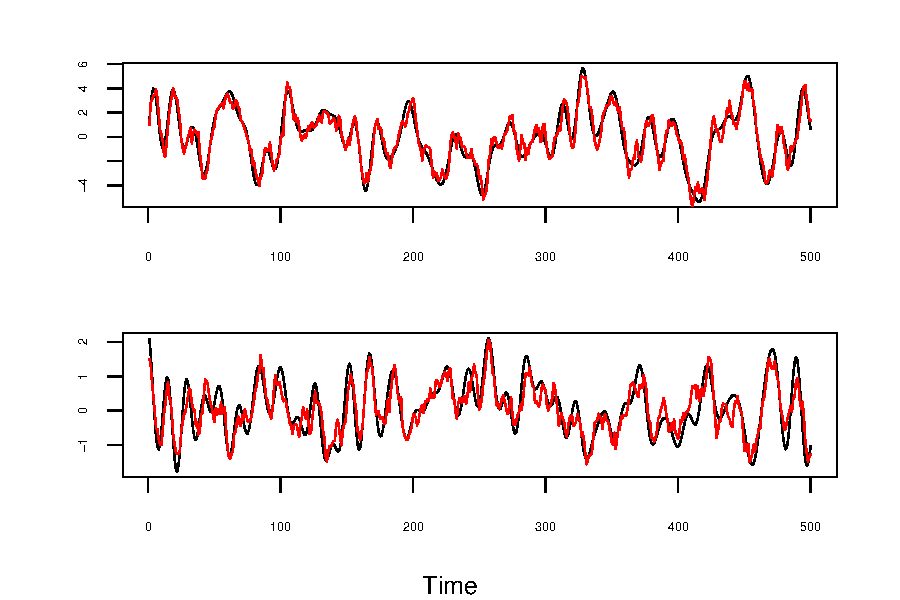
\includegraphics[]{mdfa_var1_filtering.pdf}
\end{Soutput}
\begin{Soutput}
\caption{Ideal trends (black) for the bivariate VAR(1)
	with real-time MDFA trends (red) overlaid, for series one (upper panel)
	and series two (bottom panel).
\end{Soutput}
\begin{Soutput}
\label{fig:var1.trends}}
\end{Soutput}
\begin{Soutput}
\end{center}
\end{Soutput}
\begin{Soutput}
\end{figure}
\end{Soutput}
\end{Schunk}

 Figure \ref{fig:var1.trends} shows the tracking of the ideal trends
 by the MDFA real-time trends.
The MDFA criterion  attempts to find a real-time filter $\widehat{\Psi}$
 that is close to the target $\Psi$ at frequencies that are emphasized
 by spectral content in the time series, which is assessed
 through the periodogram.   This particular 
optimization concept can be understood 
  by analyzing real-time filter outputs and filter 
  characteristics, i.e., amplitude and phase delay functions.


\begin{Exercise} {\bf MDFA VAR(1) Filtering Characteristics.} \rm
\label{exer:var1mdfa2.filter}
 This exercise examines MDFA applied to the trend of a trivariate VAR(1) process,
 which is essentially three univariate AR(1) processes.
Simulate a sample of size $T=2500$ from a
 trivariate VAR(1) process with 
\[
  \Phi = \left[ \begin{array}{ccc} 9/10 & 0 & 0 \\  0 & 1/10 & 0  \\ 0 & 0 & -9/10
   \end{array} \right]
\]
 and $\Sigma$ equal to the identity.   
  Apply the   ideal low-pass filter  with 
  $\mu = \pi/6$ to the sample (truncate the filter to $1000$ coefficients on each side).  
 Use the moving average filter
 MDFA  (Proposition \ref{prop:mdfa.quadsoln}) to find the best
 concurrent filter, setting $q= 12$.  Apply this concurrent filter 
 to the simulation, and compare the relevant portions to the ideal trend.
Also determine the in-sample performance, in comparison to the criterion value
 (\ref{eq:opt.val.mdfa}).
  Target the trends for both time series, and compare the results graphically.
 Finally, compute and graphically compare  the amplitude and phase delay
   functions for each of the three trend targets.
\end{Exercise}


\begin{Schunk}
\begin{Sinput}
> # Simulate a Gaussian VAR(1) of sample size 2500:
> T <- 2500
> N <- 3
> phi.matrix <- rbind(c(.9,0,0),c(0,.1,0),c(0,0,-.9))
> innovar.matrix <- diag(N)
> true.psidelta <- var1.par2psi(phi.matrix,100)
> gamma.0 <- matrix(solve(diag(N^2) - phi.matrix %x% phi.matrix) %*% 
+ 	matrix(innovar.matrix,ncol=1),nrow=N)
> x.init <- t(chol(gamma.0)) %*% rnorm(N)
> x.next <- x.init
> x.sim <- NULL
> for(t in 1:T)
+ {
+ 	x.next <- phi.matrix %*% x.next + rnorm(N)
+ 	x.sim <- cbind(x.sim,x.next)
+ }
> x.sim <- ts(t(x.sim))
> x.acf <- acf(x.sim,type="covariance",plot=FALSE,lag.max=T)[[1]]
> x.acf <- aperm(aperm(x.acf,c(3,2,1)),c(2,1,3))
> # construct and apply low pass filter
> mu <- pi/6
> len <- 1000
> lp.filter <- c(mu/pi,sin(seq(1,len)*mu)/(pi*seq(1,len)))
> lp.filter <- c(rev(lp.filter),lp.filter[-1])
> x.trend.ideal <- filter(x.sim,lp.filter,method="convolution",sides=2)[(len+1):(T-len),]
> # get MDFA concurrent filter
> q <- 20
> Grid <- T
> m <- floor(Grid/2)
> # The Fourier frequencies
> freq.ft <- 2*pi*Grid^{-1}*(seq(1,Grid) - (m+1))
> # frf for ideal low-pass
> frf.psi <- rep(0,Grid)
> frf.psi[abs(freq.ft) <= mu] <- 1
> frf.psi <- matrix(frf.psi,nrow=1) %x% diag(N) 	  
> frf.psi <- array(frf.psi,c(N,N,Grid))
> spec.hat <- mdfa.pergram(x.sim,1)	
> lp.mdfa <- mdfa.unconstrained(frf.psi,spec.hat,q)
> # apply the MDFA concurrent filter
> x.trend.mdfa11 <- filter(x.sim[,1],lp.mdfa[[1]][1,1,],method="convolution",sides=1)
> x.trend.mdfa12 <- filter(x.sim[,2],lp.mdfa[[1]][1,2,],method="convolution",sides=1)
> x.trend.mdfa13 <- filter(x.sim[,3],lp.mdfa[[1]][1,3,],method="convolution",sides=1)
> x.trend.mdfa21 <- filter(x.sim[,1],lp.mdfa[[1]][2,1,],method="convolution",sides=1)
> x.trend.mdfa22 <- filter(x.sim[,2],lp.mdfa[[1]][2,2,],method="convolution",sides=1)
> x.trend.mdfa23 <- filter(x.sim[,3],lp.mdfa[[1]][2,3,],method="convolution",sides=1)
> x.trend.mdfa31 <- filter(x.sim[,1],lp.mdfa[[1]][3,1,],method="convolution",sides=1)
> x.trend.mdfa32 <- filter(x.sim[,2],lp.mdfa[[1]][3,2,],method="convolution",sides=1)
> x.trend.mdfa33 <- filter(x.sim[,3],lp.mdfa[[1]][3,3,],method="convolution",sides=1)
> x.trend.mdfa <- cbind(x.trend.mdfa11 + x.trend.mdfa12 + x.trend.mdfa13,
+ 	x.trend.mdfa21 + x.trend.mdfa22 + x.trend.mdfa23,
+ 	x.trend.mdfa31 + x.trend.mdfa32 + x.trend.mdfa33)
> x.trend.mdfa <- x.trend.mdfa[(len+1):(T-len),] 
\end{Sinput}
\end{Schunk}


\begin{Schunk}
\begin{Sinput}
> # compare in-sample performance
> print(c(mean((x.trend.ideal[,1] - x.trend.mdfa[,1])^2),
+ 	mean((x.trend.ideal[,2] - x.trend.mdfa[,2])^2),
+ 	mean((x.trend.ideal[,3] - x.trend.mdfa[,3])^2)))
\end{Sinput}
\begin{Soutput}
[1] 0.28659923 0.08267115 0.01658807
\end{Soutput}
\begin{Sinput}
> # compare to criterion value
> diag(lp.mdfa[[2]])
\end{Sinput}
\begin{Soutput}
[1] 0.27735208 0.08286560 0.02052104
\end{Soutput}
\begin{Sinput}
> # compute gain and phase delay functions
> frf.psi <- frf.psi[1,1,]
> gain.psi <- abs(frf.psi)
> phased.psi <- Arg(frf.psi)/freq.ft
> lp.frf <- mdfa.frf(lp.mdfa[[1]],0,T)
> lp.gain1 <- abs(lp.frf[1,1,])
> lp.gain2 <- abs(lp.frf[2,2,])
> lp.gain3 <- abs(lp.frf[3,3,])
> lp.phased1 <- -Arg(lp.frf[1,1,])/freq.ft
> lp.phased2 <- -Arg(lp.frf[2,2,])/freq.ft
> lp.phased3 <- -Arg(lp.frf[3,3,])/freq.ft
\end{Sinput}
\end{Schunk}


\begin{Schunk}
\begin{Soutput}
\begin{figure}[htb!]
\end{Soutput}
\begin{Soutput}
\begin{center}
\end{Soutput}
\begin{Soutput}
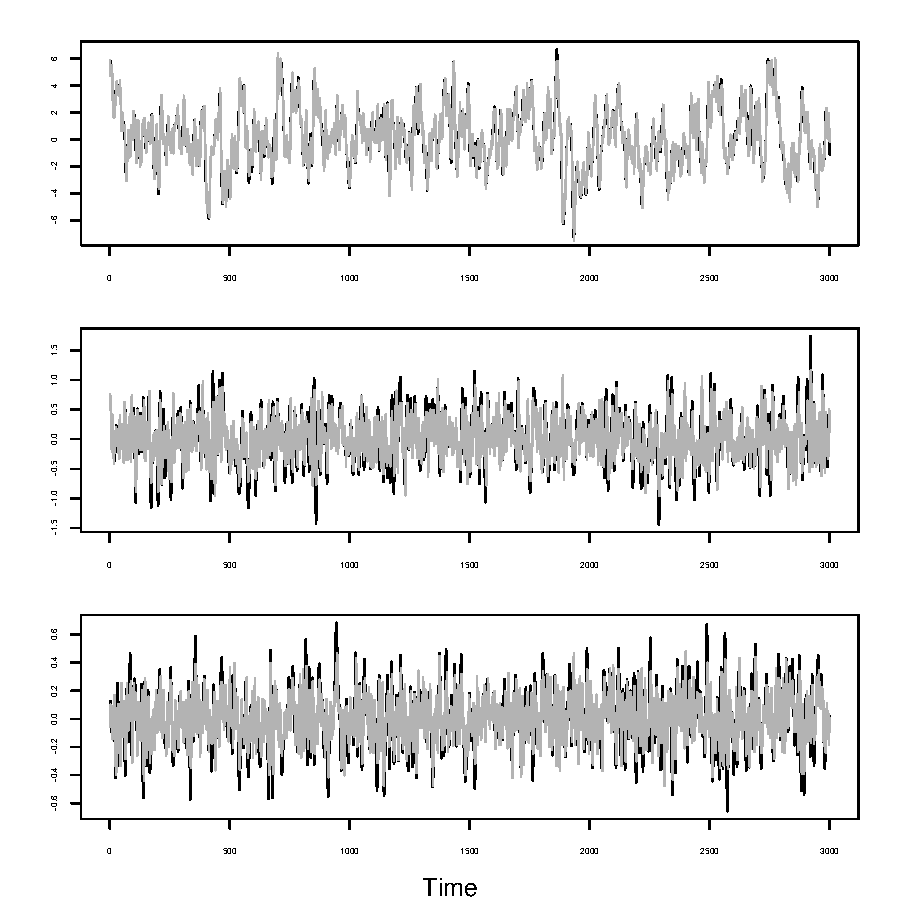
\includegraphics[]{mdfa_trivar1_filtering.pdf}
\end{Soutput}
\begin{Soutput}
\caption{Ideal trends (black) for the trivariate VAR(1)
	with real-time MDFA trends (red) overlaid, for series one (upper panel),
	series two (center panel), and series three (bottom panel).
\end{Soutput}
\begin{Soutput}
\label{fig:trivar1.trends}}
\end{Soutput}
\begin{Soutput}
\end{center}
\end{Soutput}
\begin{Soutput}
\end{figure}
\end{Soutput}
\end{Schunk}

\begin{Schunk}
\begin{Soutput}
\begin{figure}[htb!]
\end{Soutput}
\begin{Soutput}
\begin{center}
\end{Soutput}
\begin{Soutput}
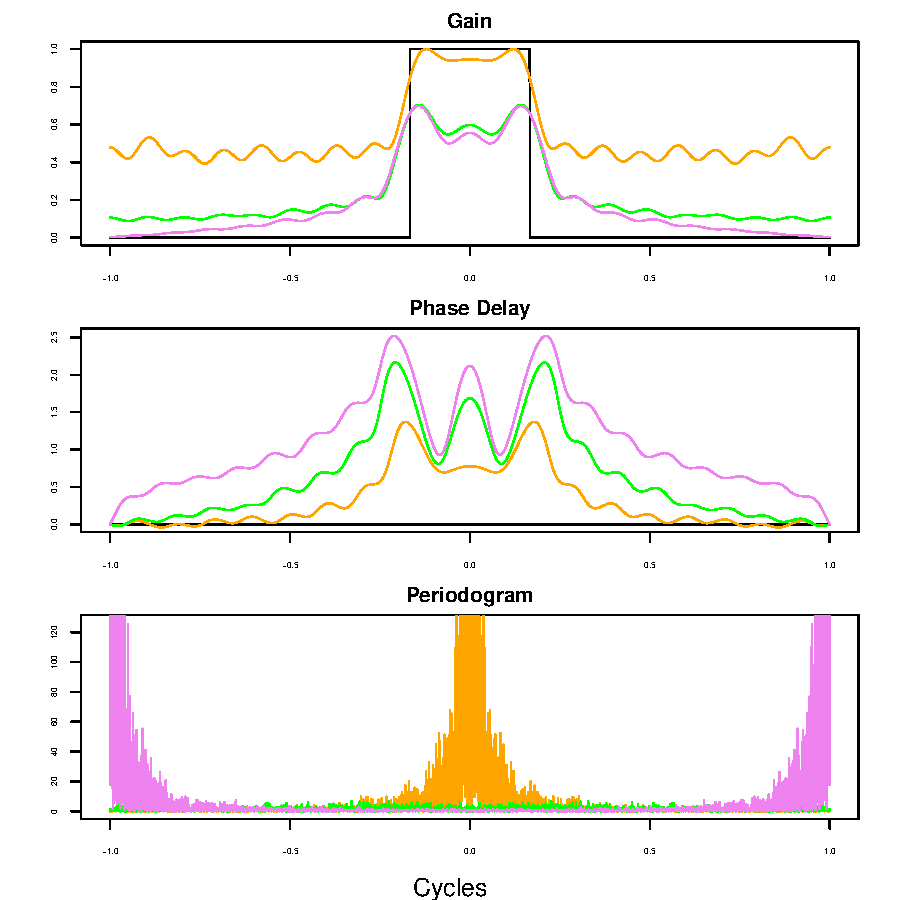
\includegraphics[]{mdfa_trivar1_freqdomain.pdf}
\end{Soutput}
\begin{Soutput}
\caption{Gain functions (upper panel), 
	Phase Delay Functions (center panel), and Periodograms (bottom panel)
	 for series one (orange), two (green), and three (violet).
\end{Soutput}
\begin{Soutput}
\label{fig:trivar1.freqdomain}}
\end{Soutput}
\begin{Soutput}
\end{center}
\end{Soutput}
\begin{Soutput}
\end{figure}
\end{Soutput}
\end{Schunk}


A visual inspection of Figure \ref{fig:trivar1.trends}, regarding
the trends and trend estimates in Exercise 
 \ref{exer:var1mdfa2.filter}, indicates an apparent conflict with the 
 criterion values: although the first series has the largest MSE,
 the fit of the concurrent estimator to the target trend appears best.
 This is because the task of the filter for the first series is
 easiest, because a higher degree of smoothness must be captured --
 whereas, in contrast, a noisy target is harder to replicate in a
 mean square error sense. Another feature is that the real-time
 estimates appear  to be systematically 
shifted to the right (they are delayed); the first series seems to be least
 affected.   These observations indicate that the difficulty of the estimation 
  task  depends on the DGP (as specified by the entries of $\Phi$):
 larger eigenvalues correspond to greater persistence of the process, 
  and an easier estimation problem.  In contrast, small eigenvalues 
 correspond to a noisier process, and a harder estimation problem.
 
 These properties are further confirmed by the gain and phase delay
 functions displayed   in Figure \ref{fig:trivar1.freqdomain}.   
 The noise  in real-time estimates $\widehat{Y}_t$  
 is due to the incomplete matching of the estimated gain (orange, green, or
 violet lines in the upper panel) to the ideal gain function (black); 
  note that the concurrent
 filters allow some   content at frequencies greater than $\mu = \pi/6$
 to penetrate.  On the other hand, the observed delay in the real-time
 estimates can be explained through the fact that the phase delay functions
 of the concurrent filters (orange, green, or
 violet lines in the center panel) do not vanish, unlike the ideal
 filter's phase delay (black).    Chapter \ref{chap:ats} 
proposes a more general optimization paradigm that will address these issues 
explicitly.

 Also observe that the phase delay function of the first series
 (orange line, center panel), which has the strongest autocorrelation,
  remains comparatively small. Its gain function (orange line, upper panel) 
 is the farthest away from the target in the stop-band $|\omega| >\pi/6$,
   but most closely resembles the target in the pass-band 
	$|\omega| \leq\pi/6$.
  Apparently,  the optimization criterion concedes
 poorer high-frequency damping to obtain improved pass-band properties. 
 In summary, $\widehat{\Psi}$ tracks $\Psi$ towards the pivotal
 frequencies, i.e., those that are important to the process'
 dynamics, as quantified by the periodogram (bottom panel) in 
 Figure \ref{fig:trivar1.freqdomain}.  
Similar findings apply to the other two series.




\section{Qualitative Easing by Leading Indicators: an Empirical Study}
   \label{sec:leading.ind}

In this section we quantify performance gains 
  obtained by inclusion of a leading indicator into a univariate design.
 In particular, consider the process
\begin{align}
 X_{t,1} & = \phi \, X_{t-1,1} + \epsilon_{t,1} \notag \\
 X_{t,2} & = X_{t+\delta,1} + \sigma \, \epsilon_{t,2}, \label{def_led_i}
\end{align} 
  where $\{ \epsilon_t \}$ is i.i.d. with mean zero and identity covariance matrix.
  Clearly, $\{ X_{t,2} \}$ is a leading indicator of $\{ X_{t,1} \}$ when
 the time-shift  $\delta > 0$.   The scaling factor $\sigma$ determines  
 the extent to which the indicator is effective, with 
 larger values of  $\sigma$ implying that the indicator is less 
informative about the target $X_{t,1}$.

\subsection{Bivariate MDFA versus Univariate DFA}
 \label{bimdfaudfa}

Here   we select $\sigma=1$, corresponding to a weak
 idiosyncratic component, and set $\delta=1$ so that the indicator
 leads by one time unit.
 

\begin{Exercise} {\bf Strong Leading Indicator.} \rm
\label{exer:bimdfa-udfa}
 Simulate a sample of size $T=200$ from the process (\ref{def_led_i}) with
 $\phi = .9$, $\delta = 1$, and $\sigma = 1$.  The target is one-step
 ahead forecasting of $\{ X_{t,1} \}$, i.e., $Y_t = X_{t+1,1}$.
  Apply univariate DFA by specializing the MDFA methodology, and compare
 to results obtained from MDFA  (Proposition \ref{prop:mdfa.quadsoln}),
 in each case setting $q=20$.  
  Apply both concurrent filters 
 to the simulation, and compare the relevant portions to the actual
 target.  Also determine the in-sample performance, in comparison to the
   criterion value  (\ref{eq:opt.val.mdfa}), for both the DFA and MDFA methods.
 Compare the results graphically.
\end{Exercise}

\begin{Schunk}
\begin{Sinput}
> # Simulate a Gaussian bivariate process of sample size 200:
> T <- 200
> N <- 2
> phi <- .9
> sigma <- 1
> gamma.0 <- 1/(1-phi^2)
> x.init <- sqrt(gamma.0)*rnorm(1)
> x.next <- x.init
> x.sim <- x.init
> for(t in 1:T)
+ {
+ 	x.next <- phi * x.next + rnorm(1)
+ 	x.sim <- c(x.sim,x.next)
+ }
> w.sim <- x.sim[-1] + sigma*rnorm(T)
> x.sim <- cbind(x.sim[-(T+1)],w.sim)
> # MDFA
> q <- 20
> Grid <- T
> m <- floor(Grid/2)
> # The Fourier frequencies
> lambda.ft <- exp(-1i*2*pi*Grid^{-1}*(seq(1,Grid) - (m+1)))
> # frf for 1-step ahead forecasting
> frf.psi <- matrix(lambda.ft^{-1},nrow=1) %x% diag(N) 	  
> frf.psi <- array(frf.psi,c(N,N,Grid))
> spec.hat <- mdfa.pergram(x.sim,1)	
> fore.mdfa <- mdfa.unconstrained(frf.psi,spec.hat,q)
> fore.udfa <- mdfa.unconstrained(frf.psi[1,1,,drop=FALSE],spec.hat[1,1,,drop=FALSE],q)
> # apply the MDFA concurrent filter
> x.fore.mdfa11 <- filter(x.sim[,1],fore.mdfa[[1]][1,1,],method="convolution",sides=1)
> x.fore.mdfa12 <- filter(x.sim[,2],fore.mdfa[[1]][1,2,],method="convolution",sides=1)
> x.fore.mdfa <- x.fore.mdfa11 + x.fore.mdfa12 
> # apply the univariate DFA concurrent filter
> x.fore.udfa <- filter(x.sim[,1],fore.udfa[[1]][1,1,],method="convolution",sides=1)
\end{Sinput}
\end{Schunk}


\begin{Schunk}
\begin{Soutput}
[1] 0.4889597 0.9915164
\end{Soutput}
\begin{Soutput}
[1] 0.597836 1.060221
\end{Soutput}
\end{Schunk}

\begin{Schunk}
\begin{Soutput}
\begin{figure}[htb!]
\end{Soutput}
\begin{Soutput}
\begin{center}
\end{Soutput}
\begin{Soutput}
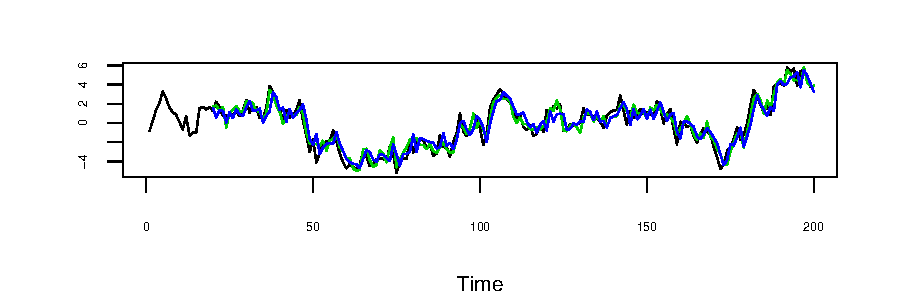
\includegraphics[]{mdfa_bimdfa-udfa.pdf}
\end{Soutput}
\begin{Soutput}
\caption{One-step ahead forecasts
 based upon MDFA (green) and univariate DFA (blue), with target in black.
\end{Soutput}
\begin{Soutput}
\label{fig:easing1}}
\end{Soutput}
\begin{Soutput}
\end{center}
\end{Soutput}
\begin{Soutput}
\end{figure}
\end{Soutput}
\end{Schunk}

We see that there is a substantial improvement to performance of the MDFA over
 the univariate DFA; this can be visualized by the tracking of the target
 shown in Figure \ref{fig:easing1}.  This is possible because the MDFA filter
 assigns more weight to the second series (the leading indicator), which is
 not available to the univariate DFA.
 

\subsection{Measuring Lead and Signal-to-Noise Effects of a Leading Indicator}
 \label{sec:lead.snr}

Intuitively, increasing $\delta$ or $\sigma$ should result in a harder forecasting
 problem: $1/ \sigma$ measures signal-to-noise ratio (snr), and low values indicate
 that real-time signal extraction becomes more difficult.  On the other hand,
 a high lead time $\delta$ requires one to do long-term forecasting, which is
 known to be hard.
 Through the fabricated  process (\ref{def_led_i}) we can disentangle the conflict
 between increasing $\delta$ and decreasing $\sigma$.
  By allowing for  non-integer shifts $\delta_j=j/4$, $j=0,1,2,3,4$
 we can quantify real-time forecasting performance.  Note
 that if the time units are annual, then the $\delta_j$ correspond to quarterly
 forecasts; more generally, taking $\delta < 1$ corresponds to now-casting
 of a time series, and has many practical applications.
  The target filter has frequency response function of the form
\[
 \Psi (e^{-i \omega}) = \exp \{ i \, \omega \delta \},
\]
 which can be immediately   implemented in the frequency domain
 (whereas in time domain, the filter is difficult to express
 when $\delta$ is non-integer).
 

\begin{Exercise} {\bf Now-casting with a Leading Indicator.} \rm
\label{exer:nowmdfa-udfa}
 Simulate a sample of size $T=2500$ from the process (\ref{def_led_i}) with
 $\phi = .9$, $\delta_j=j/4$, $j=0,1,2,3,4$ and 
$\sigma = 0,0.1,0.5,1,2$.  The target is $\delta$-step
 ahead nowcasting of $\{ X_{t,1} \}$, i.e., $Y_t = X_{t+\delta,1}$.
 Filter to obtain the now-cast target, so as to retain a target series
 of length $500$.  Combine with the leading indicator, and 
  apply univariate DFA and MDFA methodology (Proposition \ref{prop:mdfa.quadsoln}),
 in each case setting $q=20$.  
  Apply both concurrent filters 
 to the simulation, and compare the relevant portions to the actual
 target.  Record the criterion values  (\ref{eq:opt.val.mdfa})
 for both the DFA and MDFA methods.
\end{Exercise}

\begin{Schunk}
\begin{Sinput}
> # Set up loops over delta and sigma
> sigma.vals <- c(0,.1,.5,1,2)
> critmdfa.mat <- matrix(0,5,5)
> critudfa.mat <- matrix(0,5,5)
> for(delta in c(0,1,2,3,4)/4) {
+ for(j in 1:5) {
+ 
+ sigma <- sigma.vals[j]
+ # Simulate a Gaussian bivariate process of sample size 2500:
+ T <- 2500
+ N <- 2
+ phi <- .9
+ gamma.0 <- 1/(1-phi^2)
+ x.init <- sqrt(gamma.0)*rnorm(1)
+ x.next <- x.init
+ x.sim <- x.init
+ for(t in 1:T)
+ {
+ 	x.next <- phi * x.next + rnorm(1)
+ 	x.sim <- c(x.sim,x.next)
+ }
+ 
+ Grid <- T
+ m <- floor(Grid/2)
+ # define complex exponential at Fourier frequencies
+ lambda.ft <- exp(-1i*2*pi*Grid^{-1}*(seq(1,Grid) - (m+1)))
+ # frf for delta-step ahead forecasting
+ frf.psi <- matrix(lambda.ft^{-delta},nrow=1) 
+ frf.psi <- array(frf.psi,c(1,1,Grid))
+ nowcast.filter <- mdfa.coeff(frf.psi,-len,len)
+ x.target <- filter(x.sim,nowcast.filter[1,1,],method="convolution",sides=2)[(len+1):(T-len)]
+ w.sim <- x.target + sigma*rnorm(T-2*len)
+ x.sim <- cbind(x.sim[(len+1):(T-len)],w.sim)
+ 
+ # MDFA
+ q <- 20
+ Grid <- T - 2*len
+ m <- floor(Grid/2)
+ # The Fourier frequencies (recompute with smaller sample size)
+ lambda.ft <- exp(-1i*2*pi*Grid^{-1}*(seq(1,Grid) - (m+1)))
+ # frf for delta-step ahead forecasting
+ frf.psi <- matrix(lambda.ft^{-delta},nrow=1) %x% diag(N)
+ frf.psi <- array(frf.psi,c(N,N,Grid))
+ spec.hat <- mdfa.pergram(x.sim,1)	
+ fore.udfa <- mdfa.unconstrained(frf.psi[1,1,,drop=FALSE],spec.hat[1,1,,drop=FALSE],q)
+ if(j > 1) { 
+ 	fore.mdfa <- mdfa.unconstrained(frf.psi,spec.hat,q) 
+ } else {
+ 	fore.mdfa <- fore.udfa 
+ }
+   
+ # apply the MDFA concurrent filter
+ x.fore.mdfa11 <- filter(x.sim[,1],fore.mdfa[[1]][1,1,],method="convolution",sides=1)
+ if(j > 1) { 
+ 	x.fore.mdfa12 <- filter(x.sim[,2],fore.mdfa[[1]][1,2,],method="convolution",sides=1) 
+ } else { x.fore.mdfa12 <- 0*x.fore.mdfa11 }
+ x.fore.mdfa <- x.fore.mdfa11 + x.fore.mdfa12 
+ 
+ # apply the univariate DFA concurrent filter
+ x.fore.udfa <- filter(x.sim[,1],fore.udfa[[1]][1,1,],method="convolution",sides=1)
+ 
+ # compare in-sample performance
+ print(c(mean((x.target[-seq(1,q-1)] - x.fore.mdfa[-seq(1,q-1)])^2),
+ 	mean((x.target[-seq(1,q-1)] - x.fore.udfa[-seq(1,q-1)])^2)))
+ 
+ # store criterion value
+ i <- delta*4 + 1
+ critmdfa.mat[i,j] <- fore.mdfa[[2]][1,1]
+ critudfa.mat[i,j] <- fore.udfa[[2]][1,1]
+ }}
\end{Sinput}
\begin{Soutput}
[1] 2.303443e-27 2.303443e-27
[1] 1.220660e-23 3.009526e-27
[1] 2.995112e-27 2.584479e-27
[1] 2.022901e-27 1.977903e-27
[1] 2.858602e-27 2.838548e-27
[1] 0.06592913 0.06592913
[1] 0.006718234 0.049216449
[1] 0.04534792 0.06389824
[1] 0.05256748 0.06008078
[1] 0.06072431 0.06343904
[1] 0.2761297 0.2761297
[1] 0.009799982 0.283277292
[1] 0.1138029 0.2977532
[1] 0.2052450 0.2721752
[1] 0.2529586 0.2886426
[1] 0.6335297 0.6335297
[1] 0.008103726 0.577454550
[1] 0.1497622 0.5870071
[1] 0.3736056 0.6285369
[1] 0.5586076 0.7062179
[1] 0.938088 0.938088
[1] 0.01018137 0.84562243
[1] 0.1938066 1.0069663
[1] 0.4549477 0.9751027
[1] 0.7982452 1.0766016
\end{Soutput}
\end{Schunk}

\begin{Schunk}
\begin{Sinput}
>   xtable(critmdfa.mat, dec = 1,digits=rep(3,dim(critmdfa.mat)[2]+1),
+   paste("Effect of lead and  inverse signal-to-noise ratio on MDFA filter MSE",sep=""),
+   label=paste("tab:critmdfa.mat",sep=""),
+   center = "centering", file = "", floating = FALSE)
\end{Sinput}
\begin{Soutput}
% latex table generated in R 3.5.0 by xtable 1.8-3 package
% Tue May 14 18:47:44 2019
\begin{table}[ht]
\centering
\begin{tabular}{rrrrrr}
  \hline
 & 1 & 2 & 3 & 4 & 5 \\ 
  \hline
1 & -0.000 & 0.000 & -0.000 & -0.000 & 0.000 \\ 
  2 & 0.064 & 0.007 & 0.048 & 0.055 & 0.060 \\ 
  3 & 0.280 & 0.023 & 0.122 & 0.203 & 0.266 \\ 
  4 & 0.623 & 0.009 & 0.152 & 0.370 & 0.583 \\ 
  5 & 0.950 & 0.048 & 0.201 & 0.455 & 0.797 \\ 
   \hline
\end{tabular}
\caption{Effect of lead and  inverse signal-to-noise ratio on MDFA filter MSE} 
\label{tab:critmdfa.mat}
\end{table}
\end{Soutput}
\end{Schunk}
 
\begin{Schunk}
\begin{Sinput}
>   xtable(critudfa.mat, dec = 1,digits=rep(3,dim(critudfa.mat)[2]+1),
+   paste("Effect of lead and  inverse signal-to-noise ratio on DFA filter MSE",sep=""),
+   label=paste("tab:critudfa.mat",sep=""),
+   center = "centering", file = "", floating = FALSE)
\end{Sinput}
\begin{Soutput}
% latex table generated in R 3.5.0 by xtable 1.8-3 package
% Tue May 14 18:47:44 2019
\begin{table}[ht]
\centering
\begin{tabular}{rrrrrr}
  \hline
 & 1 & 2 & 3 & 4 & 5 \\ 
  \hline
1 & -0.000 & -0.000 & -0.000 & 0.000 & -0.000 \\ 
  2 & 0.064 & 0.050 & 0.067 & 0.063 & 0.063 \\ 
  3 & 0.280 & 0.297 & 0.291 & 0.272 & 0.306 \\ 
  4 & 0.623 & 0.566 & 0.574 & 0.626 & 0.731 \\ 
  5 & 0.950 & 0.851 & 1.027 & 0.973 & 1.080 \\ 
   \hline
\end{tabular}
\caption{Effect of lead and  inverse signal-to-noise ratio on DFA filter MSE} 
\label{tab:critudfa.mat}
\end{table}
\end{Soutput}
\end{Schunk}

 The results for MDFA and univariate DFA, respectively, are given in 
Tables \ref{tab:critmdfa.mat} and \ref{tab:critudfa.mat}.
Regarding the design of Exercise \ref{exer:nowmdfa-udfa}, we make the following 
comments.  When $\sigma = 0$ the leading indicator exactly matches the target;
 if $\delta = 0$ as well, then $X_{t,1} = X_{t,2}$ and there is redundancy in
 the data -- this will lead to a singularity in the periodogram.  When 
 $\delta > 0$ (but $\sigma = 0$) then $\{ X_{t,1} \}$ and $\{ X_{t,2} \}$
 are perfectly coherent, as the relation $X_{t,2} = B^{-\delta} \, X_{t,1}$ holds.
 This full coherency indicates a type of redundancy is still present,
 and the MDFA method is singular.  Therefore, in these cases we restrict
 the MDFA to univariate DFA.  Therefore, the first columns of 
 Tables \ref{tab:critmdfa.mat} and \ref{tab:critudfa.mat} are identical.

 The first rows of Tables \ref{tab:critmdfa.mat} and \ref{tab:critudfa.mat}
 are trivially zero, because when $\delta = 0$ the target is observable,
 and hence both MDFA and DFA select the identity filter.  
 Broadly, the patterns are what we would expect: increasing $\delta$ and/or
 $\sigma$ generates worse performance (higher MSE), although the MDFA is
 superior to DFA.  The performance of MDFA relative to DFA worsens as 
 $\sigma$ increases, irrespective of $\delta$, which makes sense: there
 is less benefit to the leading indicator when the snr is low, in which
 case DFA should generate a competitive real-time filter.
  In particular, reading across the rows of Table \ref{tab:critudfa.mat}
 we see the MSE is fairly constant -- DFA does not utilize the leading indicator,
 so the variability here is due to the simulation seeds.
  As for the MDFA, decreased performance due to lower snr could be 
 compensated by decreasing the lead-time $\delta$.  
  Again, when $\sigma$ is low (second column of Table \ref{tab:critmdfa.mat})
  the leading indicator is very useful, and the MSE does not depend 
 greatly on $\delta$.  This pattern is opposite when $\sigma$ is high 
 (fifth column), as increased $\delta$ deleteriously affects performance.

   
These results suggest the pertinence of a mixed-frequency approach,
 whereby information at differing sampling frequencies (such as monthly
 and quarterly data) is combined.  The higher-frequency data stream
 could be used to update the filter for the lower-frequency time series;
 this is further discussed in Chapter \ref{chap:mix}. 
 

%\SweaveInput{Mean_square}
%  note: MDFA_basic replaces Mean_square

%----------------------------------------



\chapter{Multivariate Direct Filter Analysis for Non-stationary Processes}
\label{chap:int}

 We now extend the basic MDFA of Chapter \ref{chap:basic}  by considering
 the method's application to  non-stationary processes.  
 Section \ref{sec:constraint} introduces the idea of filter constraints
arising from time-varying means, a form of non-stationarity.
 This treatment is generalized in Section \ref{sec:non-stat}
  by the definition of non-stationary processes, and theory for the corresponding
   model-based filters is developed.  Finally, the MDFA criterion for
    non-stationary processes is discussed in Section \ref{sec:mdfa-nonstat}.
 
   
% Section \ref{i1i2_intr} sets-up the context; a link to integrated processes is proposed in 
% section \ref{pseudo_dft}; a general matrix notation is proposed in 
% section \ref{cons_gen_par}; section \ref{optim_stat} extends the former 
% (unconstrained) MDFA-criterion to the constrained case; finally, section 
% \ref{const_impl_mdfa} illustrates effects (of the constraints) on 
%  characteristics of real-time filters.  



\section{Constrained MDFA}
\label{sec:constraint}

 Various constraints upon the concurrent filter can be envisioned, 
   and imposing such strictures results in  a constrained MDFA. 
   A chief case of interest arises when the 
    data process has a time-varying mean (which is a form of  non-stationarity);
  then it is necessary to impose additional filter constraints -- otherwise
   the filter error will not have mean zero.    To see why, 
   Write $\Delta (L) = \Psi (L) - \widehat{\Psi} (L)$ as the discrepancy filter,
   so that we see  from (\ref{eq:dfa-error})  
   that $\EE [ E_t ] = \Delta (L) \, \EE [ X_t ]$; 
   by Definition \ref{def:lpp}, we require
 that $\EE [ E_t ] = 0$ for any LPP.  
  If $\EE [ X_t] = 0$ then this condition is always satisfied, but
   for most time series of interest the mean will be nonzero, and is typically
    time-varying.  For such cases additional constraints on $\Delta (L)$ must be imposed,
    which implicitly amount to constraints on $\widehat{\Psi} (L)$.
    
\begin{Example}    {\bf Constant Mean.}  \rm
\label{exam:constant.mean}
  If $\EE [ X_t ] = \mu$, some nonzero constant,  then we require $\Delta (1) = 0$.
  This is because the mean of the filter error is
  \[
   \Delta (B) \, \EE [ X_t] = \Delta(B) \, \mu = \sum_j \delta (j) \, \mu =
   \Delta (1) \, \mu,
  \]
  and this is zero only if $\Delta (1) = 0$.  This is called a Level Constraint (LC).
\end{Example}  

\begin{Example}    {\bf Linear Mean.}  \rm
\label{exam:linear.mean}
  Suppose that $\EE [ X_t ] = \mu \, t$, where $\mu$ is a nonzero slope
 of a linear time trend.  Then it is required that  $\partial {\Delta} (1) = 0$
  in addition to the LC,  which is seen as follows:
  \[
   \Delta (B) \, \EE [ X_t] = \Delta(B) \, \mu \, t =   \mu \, \sum_j \delta (j) \, (t-j)
   = \mu \, \left(t \, \sum_j \delta (j) - \sum_j j \,\delta (j) \right)
    = \mu \, t \, \Delta(1) - \mu \, \partial \Delta (1).
  \]
  This mean of the filter error  is zero only if both $\Delta(1)=0$ and
  $\partial \Delta (1)=0$; the latter condition is called the
   Time-Shift Constraint (TSC).  
\end{Example}  

     Hence, for linear means we obtain
 three fundamental types of constraints: LC, TSC, and Level plus 
 Time-Shift Constraint (LTSC), which combines both LC and TSC.
  Using the fact that $\Delta (L) = \Psi (L) - \widehat{\Psi} (L)$,
   these three constaints can be described as follows:
\begin{align*}
 \mbox{LC} : &  \;  \Delta (1) = 0 \quad \mbox{or} \quad \Psi (1) = \widehat{\Psi} (1) \\
 \mbox{TSC} : &  \;   \partial {\Delta} (1) = 0 \quad \mbox{or} \quad 
 \partial {\Psi} (1) = \partial {\widehat{\Psi}} (1)  \\
 \mbox{LTSC} : &  \;  \Delta (1) = 0,  \,  \partial {\Delta} (1) = 0 \quad 
 \mbox{or} \quad \Psi (1) = \widehat{\Psi} (1), \; \partial {\Psi} (1) =
 \partial {\widehat{\Psi}} (1).
\end{align*}
 In the case of  concurrent filters of form  (\ref{eq:conc.filter}), 
 LC is accomplished by demanding that 
  $\sum_{j=0}^{q-1} \widehat{\psi} (j) = \Psi(1)$.   More generally, we consider  linear constraints  formulated via
\begin{equation}
\label{eq:concurrent-constrain}
  \vartheta = R \, \varphi + Q,
\end{equation}
 where $R$ is $n q \times n r$ and $\varphi$ is $n r \times 1$ dimensional, consisting of 
 free parameters; $Q$ is a matrix of constants, and is $n q \times 1$ dimensional.


\begin{Illustration}  {\bf Level Constraint (LC).}   \rm
\label{ill:lc}
 Note that $\sum_{j=0}^{q-1} \widehat{\psi} (j) = \Psi(1)$ implies that
\begin{equation}
\label{eq:lc-gamma0}
 \widehat{\psi} (0) = \Psi(1) - \sum_{j=1}^{q-1} \widehat{\psi} (j).
\end{equation}
 Hence  $ \varphi^{\prime}  = [ \widehat{\psi} (1), \widehat{\psi} (2), \ldots, \widehat{\psi} (q-1) ] $ and
\[
	R  = \left[ \begin{array}{ccc} -1 & \ldots & -1 \\ 1 & 0 & 0 \\
		\vdots & \ddots & \vdots \\ 0 & 0 & 1  \end{array} \right]  \otimes 1_n \qquad
	Q = \left[ \begin{array}{c} \Psi (1) \\ 0 \\ \vdots \\ 0 \end{array} \right].
\]
\end{Illustration}
 
 
\begin{Illustration}  {\bf Time Shift Constraint (TSC).}   \rm
\label{ill:tsc}
   The constraint is $\partial {\Psi} (1) = \partial \widehat{\Psi} (1)
   = \sum_{j=0}^{q-1} j \, \widehat{\psi} (j)$,
 or $\widehat{\psi} (1)  = \partial {\Psi} (1)  -  \sum_{j=2}^{q-1} j \, \widehat{\psi} (j) $.
 Hence  $ \varphi^{\prime}  = [ \widehat{\psi} (0), \widehat{\psi} (2), \ldots, \widehat{\psi} (q-1) ] $ and
\[
	R  = \left[ \begin{array}{cccc} 1 & 0 &  \ldots &  0  \\  0 & -2  &  -3  & \ldots  \\
		0 & 1 & 0 & \ldots \\ 
		\vdots & \ddots & \vdots & \vdots \\ 0 & \ldots & 0 & 1 \end{array} \right] \otimes 1_n \qquad
	Q = \left[ \begin{array}{c} 0 \\ \partial {\Psi} (1) \\ 0 \\ \vdots \\ 0 \end{array} \right].
\]
\end{Illustration}
 
 
\begin{Illustration}  {\bf Level and Time Shift Constraint (LTSC).}  \rm
\label{ill:ltsc}
   Take the Time Shift Constraint formula for $\widehat{\psi} (1)$,
 and plug this into (\ref{eq:lc-gamma0}), to obtain
\begin{align*}
 \widehat{\psi} (0)  & = \Psi (1) - \left( \partial {\Psi} (1)  -  \sum_{j=2}^{q-1} j  \, \widehat{\psi} (j) \right) -  \sum_{j=2}^{q-1} 
 \widehat{\psi} (j)  \\
	& = \Psi (1) -  \partial {\Psi} (1)  +  \sum_{j=2}^{q-1} (j-1)  \, \widehat{\psi} (j).
\end{align*}
 Hence  $ \varphi^{\prime}  = [  \widehat{\psi} (2), \ldots, \widehat{\psi} (q-1)  ] $ and
\[
	R  = \left[ \begin{array}{cccc} 1 & 2  &  3  &   \ldots    \\  -2  & -3  &  -4  & \ldots  \\
		 1  & 0 & \ldots & 0 \\ 
		\vdots & \ddots & \vdots & \vdots \\ 0 & \ldots & 0 & 1 \end{array} \right]  \otimes 1_n \qquad
	Q = \left[ \begin{array}{c} \Psi (1) - \partial {\Psi} (1)  \\  \partial {\Psi} (1) \\ 0 \\ \vdots \\ 0 \end{array} \right].
\]
\end{Illustration}



 More generally, we can envision an LPP involving $M$ linear constraints on 
  $\vartheta$, taking the form
 $   A = [ J \otimes 1_n ] \, \vartheta$, where $J$ is $M \times q$ 
 dimensional ($M < q$) and $A$ is $n M \times 1$ dimensional.
 (The LC, TSC, and LTSC examples all have this form.)  In order to express 
 this constraint in the form 
 (\ref{eq:concurrent-constrain}), we use the Q-R decomposition 
 (Golub and Van Loan, 1996) of $J$, writing
 $J = C \, G \, \Pi$ for an orthogonal matrix $C$ (which is $M \times M$ dimensional),
 a rectangular upper triangular matrix $G$
 (which is $M \times q$ dimensional), and a permuation matrix $\Pi$ 
 (which is $q \times q$ dimensional).  
 Standard matrix software such as $\textsc{R}$ will provide the Q-R decomposition $J$,
 and should produce the rank of $J$ as  a by-product --
 if this is less than $M$, then there are redundancies in the 
 constraints that should first be eliminated. 
 
 \begin{Exercise} {\bf QR Decomposition.} \rm
 \label{exer:qr.constraint}
 TO DO
 \end{Exercise}
 
 Hence  proceeding with a full rank $J$, we partition $G$ as $G = [ G_1 \, G_2]$ 
 such that $G_1$ has $M$ columns and $G_2$
 has $q-M$ columns.  This quantity $q-M$ corresponds to the number 
 of free coefficient matrices, and is therefore the same as $r$.
 The Q-R decomposition guarantees that $G_1$ is an upper triangular matrix, 
 and moreover it is invertible.  Therefore
\[
  \left[ G_1^{-1} \, C^{-1} \otimes 1_N \right] \, A  = \left( \left[ 1_M , \, G_1^{-1} \, G_2 \right] \, \Pi \otimes 1_N  \right) \, \vartheta,
\]
 and the action of $\Pi$ (together with the tensor product) amounts 
 to a   permutation of the elements of $\vartheta$.
  Let the output of this permutation be denoted
\[
   \left[ \begin{array}{l} \overline{\vartheta} \\ \underline{\vartheta} \end{array} \right]
   = \left( \Pi \otimes 1_N \right) \, \vartheta,
\]
 where $\overline{\vartheta}$ is $N M \times 1$ dimensional and
 $\underline{\vartheta}$ is $N r \times 1$ dimensional.  
 Then  by substitution we can solve for $\overline{\vartheta}$ in terms 
 of $\underline{\vartheta}$:
\[
   \overline{\vartheta} =  \left[ G_1^{-1} \, C^{-1} \otimes 1_N \right] \, A - 
   \left[  G_1^{-1} \, G_2  \otimes 1_N   \right] \, \underline{\vartheta}.
\]
 Therefore we recognize the free variables $\varphi = \underline{\vartheta}$, 
 and obtain $R$ and $Q$ in (\ref{eq:concurrent-constrain}) via
\begin{align*}
   R & = \Pi^{-1} \, \left[ \begin{array}{c} - G_1^{-1} \, G_2 \\ 1_{r} \end{array} \right] \otimes 1_N  \\
  Q & = \left( \Pi^{-1}  \, \left[ \begin{array}{c}  G_1^{-1} \, C^{-1} \\ 0 \end{array} \right] \otimes 1_N  \right) \, A.
\end{align*}
  These formulas allow one to compute the   form (\ref{eq:concurrent-constrain}) 
   from given constraints, and
 an analytical solution to the resulting MDFA criterion  be obtained from the following result.

\begin{Proposition}
\label{prop:mdfa.quadsoln-constrain}
 The minimizer of the  MDFA criterion given by   (\ref{eq:mdfa-criterion})
 with respect to  $\mathcal{G}$ -- consisting of all length $q$ concurrent filters 
 subject to  linear constraints of the form (\ref{eq:concurrent-constrain}) -- is
\begin{equation}
\label{eq:phi.soln-constained}
 \varphi =  { \left[ R^{\prime} \, B \, R \right] }^{-1} \, R^{\prime} \,
 \left( b - B \, Q \right).
\end{equation}
  Letting $H = 1_{Nq} - R \,   { \left[ R^{\prime} \, B \, R \right] }^{-1} \,
  R^{\prime} \, B$, the minimal value is  
\begin{equation}
\label{eq:opt.val.mdfa-constrained}
{ \langle \Psi (z) \, G \, { \Psi (z) }^* \rangle }_0 - b^{\prime} \, 
R \, { \left[ R^{\prime} \, B \, R \right] }^{-1} \, R^{\prime} \,  b
	+ Q^{\prime} \, B \, H \, Q - 2 \, b^{\prime} \, H \, Q.
\end{equation}
\end{Proposition}

For computation, we utilize the same approximations to $B$ and $b$ as discussed 
in  Chapter \ref{chap:basic},
 obtaining the constrained MDFA filter $\vartheta$ via (\ref{eq:phi.soln-constained})
 followed by (\ref{eq:concurrent-constrain}).

HERE  add exercise on ideal low-pass with various constraints 
  for a WN process with linear trend.  
 repeat with VAR(1) with linear trend

% 
% We suppose the true process is a VAR($1$), and apply the MB trend filter defined in Example \ref{exam:trend-i1},
%   where the parameters are given by
% \[
%  \Sigma_{\mu} = \left[ \begin{array}{ll} 
%    2.32 \cdot 10^{-4} &  5.04 \cdot 10^{-4} \\
%    5.04 \cdot 10^{-4}  & 34.73 \cdot 10^{-4}  \end{array}  \right]
%  \qquad  \Sigma_{\iota} = \left[ \begin{array}{ll}
%         110.44 \cdot 10^{-5} &  7.17 \cdot 10^{-5}  \\
%         7.17 \cdot 10^{-5} & 128.57 \cdot 10^{-5}   \end{array} \right].
% \]
%   Because the trend variance for the second component is $15$ times larger than that of the first component,
%  the correspoding trend filter  does less smoothing.  
%  
% \begin{figure}[htb!]
% \centering
% \includegraphics[]{petrolVAR1trends}
% \caption{\baselineskip=10pt Bivariate  trend  filter applied to VAR($1$) simulation (grey), with trends in black. }
% \label{fig:petrol.var1trends}
% \end{figure}
% 
% 
%   We seek to solve the corresponding trend extraction LPP.    First, we can use the optimal solution  (\ref{eq:var1.lpp-opt})
% given in   Illustration \ref{ill:var1}, supposing that we know  that the VAR($1$) is correctly specified.  
%  Second, we can use MDFA, proceeding as if we do not know the true process is a VAR($1$), as we would in practice, 
% and hence use the periodogram;  MDFA should be able to replicate the optimal solution, so long as the filter class
%  $\mathcal{G}$ is sufficiently rich.    The VAR($1$)  is defined by
% \[
%   X_t =  \left[ \begin{array}{ll}  1.0  & 0.5 \\    -0.2  &  0.3  \end{array} \right] \, X_{t-1} + \epsilon_t,
% \]
%  with stationary initialization, and $\{ \epsilon_t \}$ a Gaussian white noise of identity innovation variance.
%   Operationally, we simulate this process with sample size $4500$.  Then the 
%   ideal trends $\Psi (B) X_t$ are produced by truncating the  MB  filter to length $4001$ (it is symmetric, so the indices
%  range between $-2000$ and $2000$) and applying to the  simulation, only retaining the central $500$ data points,
%  as displayed in Figure \ref{fig:petrol.var1trends}.   (In this way we can dispense with edge effects, and the extra
%  $4000$ observations are not used in the MDFA.)     The grey lines of Figure \ref{fig:petrol.var1trends}
%  are the central $500$ observations of the VAR($1$)
%  simulation, and the  black  line is the target.     We wish to use MDFA (setting $q=30$) 
%  with various constraints (LC, TSC, LTSC) 
% to obtain a   real-time estimate,  comparing  the result  to the optimal solution given by implementing  Illustration \ref{ill:var1}.  
%   In that case  we find that
% \[
%   A_{\Psi} (\Phi) = \left[ \begin{array}{ll}  0.317  &  0.218 \\    -0.054  &  0.027  \end{array} \right]
% \]
%  by direct calculation, 
% and hence the optimal filter is easily computed.  The in-sample MSEs of the various methods are displayed in Table \ref{tab:petrol.var1.mdfa}.
%   Note that the basic MDFA (no constraints) replicates the optimal filter, as their MSE is the same up to negligible   error.
%   When imposing a level constraint (LC and LTSC) there is a loss to the MDFA performance, which makes sense given that the optimal
%  filter does {\it not} impose a level constraint -- in fact, the value of the optimal concurrent filter at frequency zero is
% \[
%   \widehat{\Psi} (1) =  \left[ \begin{array}{ll}  0.914 &  0.251 \\    -0.030  &  0.842  \end{array} \right],
% \]
%  which is quite different from $1_2$.  On the other hand, the time shift constraint alone (TSC) has little impact on the performance of MDFA,
%  because $\partial \widehat{\Psi} (1) \approx 0 \cdot 1_2$, i.e., the optimal filter already has this property of zero time shift.
% 
%  
% 
% \begin{table}[!htb]
% \centering
% \begin{tabular}{clllll}
% \hline
%   Series  &  LPP Opt  &  MDFA Basic &  MDFA LC &  MDFA TSC   &  MDFA LTSC \\
%   1 & .2404  &  .2388  &  .2877  &   .2363  & .4367  \\
%   2 & .0224 &   .0217 &   .0229  &   .0216  & .0264 \\
% \hline
% \end{tabular}
% \caption{\baselineskip=10pt  LPP MSE for bivariate VAR($1$) process --  with target trend
%  given by the LLM MB trend -- for various concurrent filters: LPP Opt is the optimal filter,
%  whereas the MDFA filters are labeled according to the constraints imposed. }
% \label{tab:petrol.var1.mdfa}
% \end{table}
%  




\section{Background on Non-stationary Vector Time Series }
\label{sec:non-stat}

We next consider processes that when differenced are 
stationary, which are the most common type occuring in econometrics and finance.  
 This type of non-stationary process substantially broadens
  the possible types of applications over the stationary processes
   considered in Chapters \ref{chap:lpp} and \ref{chap:basic}.
  Also, as such processes typically can have a time-varying mean,
  they also necessitate the use of filter constraints such as those
   considered in Section \ref{sec:constraint}.
  
 We suppose that there exists a polynomial $\delta (L)$
  that reduces each component series of $\{ X_t \}$ to a stationary
   time series (which is allowed to have a non-zero constant mean),
   and suppose this is the minimal degree polynomial that accomplishes
    this reduction.  We write $\partial X_t = \delta (L) \, X_t$ for
  the stationary, differenced time series.
    
HERE :  do examples with $1-L$  and $1-L^2$, derive time-varying
  spectral rep (from old notes on evol spectra, and DFA paper).
  
  
  HERE : state the following as a proposition
    
So we can write
\[
 X_t = \sum_{j=1}^d A_{j, t+d} \, X_{j-d} + \int_{-\pi}^{\pi}
 \frac{ e^{i \omega t} - \sum_{j=1}^d A_{j,t+d} \, e^{-i \omega
 (d-j)} }{ \delta (e^{-i \omega}) } \; d \ZZ (\omega),
\]
 where $d = \sum_{\ell=1}^m q_{\ell}$ and each $A_{j, t+d}$ is a
 time varying function for each $j$, and the $x_{j-d}$ are initial
 values.  This representation is chiefly useful when $t > 1$, though
 it is still valid when $t \leq 0$.  The $\ZZ (\omega)$ is the
 orthogonal increments process in the spectral representation of
 $\partial X_t$. 

 Each of the time-varying functions is in the null
 space of $\delta (B)$, i.e., $\delta (B) A_{j, t+d} = 0$ for $1 \leq
 j \leq d$, where the backshift operator works on the $t+d$ index.
 As a consequence, we can rewrite each $A_{j,t+d}$ as a linear
 combination of the basis functions of the null space of $\delta
 (B)$, which yields a more convenient representation.  Let the basis
 functions be $\phi_j (t) $ for $1 \leq j \leq d$; the existence and
 form of such functions are a basic staple of difference equation
 theory, treated briefly in Brockwell and Davis (1991).  Then we can
 write $A_{j,t+d} = \sum_{k=1}^d G_{jk} \phi_k (t)$ for each $1 \leq
 j \leq d$, for some coefficients $G_{jk}$.  It follows that
\[
 \sum_{j=1}^d A_{j,t+d} B^{d-j} = \sum_{k=1}^d \phi_k (t)  \; \left(
 \sum_{j=1}^d G_{jk} B^{d-j} \right).
\]
 Each expression in parentheses on the right hand side is a degree
 $d-1$ polynomial in $B$, and will henceforth be denoted as $p^{(k)}
 (B)$.   Substituting the new formulation, we obtain
\[
 x_t = \sum_{j=1}^d \phi_j (t) p^{(j)} (B) \, x_{0} + \int_{-\pi}^{\pi}
 \frac{ e^{i \omega t} - \sum_{j=1}^d \phi_j (t) \, p^{(j)} ( e^{-i \omega
 } )}{ \delta (e^{-i \omega}) } \; d \ZZ (\omega),
\]
 where $p^{(j)} (B)$ acts on $x_0$ by shifting the time index $t=0$
 back in time for each power of $B$.  This representation is now
 extremely convenient, because application of any factor of
 $\delta(B)$ will annihilate a corresponding basis function (when
 roots are repeated, some basis functions will also be transformed
 into others that are instead annihilated). 

   
  HERE material on WK : signal and noise spectra non-stat case, and basic formulas
    in freq domain
    
  HERE illustrations by LLM, STM, and Example 5 of E and S paper
  
  

\section{Error Criterion and Computation}
\label{sec:mdfa-nonstat}

HERE material from E and S paper section 4.3

% We here consider difference-stationary vector time series, which means there exists a scalar differencing polynomial $\delta (L)$ such
%  that $\partial X_t = \delta (L) X_t$ is mean zero and covariance stationary.  
%  Examination of (\ref{eq:dfa-error}) indicates that the error process is not stationary unless we make certain assumptions
%  about $\Delta (L) = \Psi (L) - \widehat{\Psi} (L)$.     It is necessary that we can factor $\delta (L)$ from $\Delta (L)$, i.e., there exists
%  $\widetilde{\Delta } (L)$ such that
% \begin{equation}
%  \label{eq:delta.factor}
%   \Delta (L) = \widetilde{\Delta } (L) \, \delta (L),
% \end{equation}
%  as otherwise we cannot guarantee that $\{ E_t \}$ will be stationary.  However, (\ref{eq:delta.factor}) is sufficient to guarantee
%  that the filter error be stationary, because
% \[
%   E_t = \widetilde{\Delta} (L) \, \partial X_t
% \]
%  in such a case.   We next discuss a set of filter constraints that guarantee (\ref{eq:delta.factor}), beginning with a lemma
%  that discusses factorization of filters.  We say a filter $\Psi (L)$ is absolutely convergent if $\sum_{j \in \ZZ} \| \psi (j) \| < \infty$
%  for a given matrix norm $\| \cdot \|$.
% 
% \begin{Proposition}
% \label{prop:filter-decompose}
%  Any linear filter $\Psi (L)$ can be expressed as
% \[
%   \Psi (L) = \Psi (\zeta) + (L - \zeta) \, \Psi^{\sharp} (L)
% \]
%  for any $\zeta \in \CC$  such that $| \zeta | = 1$, 
%   and an absolutely convergent filter $\Psi^{\sharp} (L)$, so long as  $\partial \Psi (L) $ is absolutely convergent.
%  If in addition $ \partial \partial \Psi (L) = \sum_{ j \in \ZZ} j (j-1) \, \psi (j) \, L^j$
%    is absolutely convergent, then there also exists an absolutely convergent filter $\Psi^{\flat} (L)$ 
%  such that
% \[
%  \Psi (L) = \Psi (\zeta) + \partial \Psi (\zeta) \, (L- \zeta) \, \overline{\zeta} + {(L - \zeta)}^2 \, \Psi^{\flat} (L).
% \]
% \end{Proposition}
% 
%  Note that if $\Psi (\zeta) = 0$, it follows from Proposition \ref{prop:filter-decompose} that $L-\zeta$ can be factored from
%   $\Psi (L)$.  Similarly, ${(L- \zeta)}^2$ can be factored from $\Psi (L)$ is $\Psi(\zeta) = \partial \Psi (\zeta) =0$.
% 
% \begin{Definition} \rm
% \label{def:filter-noise}
%  For $\omega \in [-\pi, \pi]$, a filter $\Psi (L)$ annihilates $\omega$-noise of order $1$ if $\Psi (e^{-i \omega}) = 0$,
%  and annihilates $\omega$-noise of order $2$ if in addition $\partial \Psi (e^{-i \omega}) = 0$.
% \end{Definition}
% 
% 
% Hence, we have the following immediate corollary of Proposition \ref{prop:filter-decompose}.
% 
% \begin{Corollary}
%  \label{cor:filter-noise}
%   If a filter $\Psi (L)$ annihilates $\omega$-noise of order $1$ and $\partial \Psi (L)$ is absolutely convergent, then
% \[
%   \Psi (L) = (L- e^{-i \omega}) \, \Psi^{\sharp} (L).
% \]
%  If a filter $\Psi (L)$ annihilate $\omega$-noise of order $2$,  and $\partial \partial \Psi (L)$ is absolutely convergent, then
% \[
%   \Psi (L) = {(L- e^{-i \omega}) }^2 \, \Psi^{\flat} (L).
% \]
% \end{Corollary}
% 
%  We can apply Corollary \ref{cor:filter-noise} to factor a noise-differencing polynomial $\delta^N (L)$ from $\Delta (L)$:
%  for each $\omega$ such that the target filter $\Psi (L)$ annihilate $\omega$-noise of order $d$, we impose the constraint
%  that $\widehat{\Psi} (L)$ shall have the same property, and hence ${(L- e^{-i \omega})}^d$ can be factored from both
%  filters.   For instance, if noise frequencies are $\omega_{\ell}$ with multiplicities $d_{\ell}$, then repeated application of 
%  Corollary \ref{cor:filter-noise} yields
% \[
%  \Psi (L) = \prod_{\ell} {(L -  e^{-i \omega_{\ell}})}^{d_{\ell}} \, \Psi^{\natural} (L)
%    = \delta^N (L) \, \Psi^{\star} (L)
% \]
%  for some residual filter $\Psi^{\natural} (L)$, where $\Psi^{\star} (L) = \prod_{\ell} -e^{-i \omega_{\ell} d_{\ell}} \, \Psi^{\natural} (L)$
%  and $\delta^N (L) = \prod_{\ell} (1 - e^{i \omega_{\ell}} \, L)$.
%  By imposing the same linear constraints on $\widehat{\Psi} (L)$, we likewise obtain $\widehat{\Psi} (L) = \delta^N (L) \, \widehat{\Psi}^{\star} (L)$,
%  and hence 
% \begin{equation}
%  \label{eq:delta-noise}
% \Delta (L) = \left(  {\Psi}^{\star} (L) - \widehat{\Psi}^{\star} (L) \right) \, \delta^N (L).
% \end{equation}
%   So if $\delta (L) = \delta^N (L)$, then (\ref{eq:delta.factor}) holds at once.  More generally, a given process' differencing polynomial
%  may be factored into relatively prime polynomials $\delta^N (z)$ and $\delta^S (z)$, which correspond to noise and signal dynamics
%  respectively -- see Bell (1984) and McElroy (2008a).  Many  signal extraction filters $\Psi (L)$   have the property that they
%  annihilate $\omega$-noise of the appropriate order, such that $\delta^N (L)$ can be factored; in addition, the noise filter $1_N - \Psi (L)$
%  has the same property with respect to the signal frequencies, i.e., $\delta^S (L)$ can be factored from $1_N - \Psi (L)$ in the same manner.
%  Hence  $1_N -  \Psi (L) =   \delta^S (L) \, \Psi^{\diamond} (L)$ for some factor $\Psi^{\diamond} (L)$,
%  and imposing the same constraints on the concurrent filter yields
% \[
%   \Delta (L) = (1_N - \widehat{\Psi} (L)) - (1_N - \Psi (L)) = \left(  \widehat{\Psi}^{\diamond} (L) - \Psi^{\diamond} (L)  \right) \, \delta^S (L).
% \]
%   However, (\ref{eq:delta-noise}) also holds, and the roots of $\delta^S (z)$ and $\delta^N (z)$ are distinct (because the polynomials
%  are relatively prime by assumption), and hence $\delta (L) = \delta^N (L) \, \delta^S (L)$ must be a factor.  Therefore,
%  $\widetilde{\Delta} (L) =  (  \widehat{\Psi}^{\diamond} (L) - \Psi^{\diamond} (L)   )/ \delta^N (L)$, and (\ref{eq:delta.factor}) holds.
% 
% In summary, given a factorization of $\delta (z)$ into signal and noise differencing polynomials, the noise constraints and signal constraints
%  on $\Psi (L)$ must also be imposed upon $\widehat{\Psi} (L)$, and this ensures that $\{ E_t \}$ will be stationary with mean zero.  
%  If $\omega$ satisfies $\delta^N (e^{-i \omega}) = 0$, then we impose that $\widehat{\Psi} (L)$ annihilates $\omega$-noise of order
%  given by the multiplicity of the root in $\delta^N (z)$.  Otherwise, if $\omega$ satisfies $\delta^S (e^{-i \omega})$ then we impose
%  that $\widehat{\Psi} (e^{-i \omega}) = \Psi (e^{-i \omega})$ (if the root is simple -- if a double root, then also impose that
%  $\partial \widehat{\Psi} (e^{-i \omega}) = \partial \Psi (e^{-i \omega})$).  In practice, we must determine the real and imaginary  parts of each such constraint, and write the corresponding constraints on $\widehat{\Psi} (L)$ in the form $A = [J \otimes 1_N] \, \vartheta$ for
%   filters of form (\ref{eq:conc.filter}), applying the methodology of the previous subsection.  
%   With these constraints in play, the formula (\ref{eq:dfa-mvar}) holds with $\Psi (z) - \widehat{\Psi} (z)$ replaced by $\widetilde{\Delta} (z)$
%  and $F$ being the spectral density of $\{ \partial X_t \}$, i.e., we define the nonstationary MDFA criterion 
%  function as $\det D_{\Psi } (\vartheta, G)$ for
% \begin{equation}
% \label{eq:mdfa-criterion-nonstat}
%  D_{\Psi} (\vartheta, G) =     { \langle  \widetilde{\Delta} (z)   \,   G \,  {\widetilde{\Delta} (z) }^*   \rangle }_0
%  = { \langle  \left[ \Psi (z) -   \widehat{\Psi}_{\vartheta} (z) \right] \,   G \, {|\delta (z) |}^{-2} \,
%   {  \left[ \Psi (z) -  \widehat{\Psi}_{\vartheta} (z) \right] }^{*} \rangle }_0.
% \end{equation}
%   The second expression in (\ref{eq:mdfa-criterion-nonstat}) utilizes (\ref{eq:delta.factor}), and employs the understanding
%  that poles in ${\delta (z) }^{-1}$ are exactly canceled out by the corresponding zeros in $\Psi (z) - \widehat{\Psi} (z)$.
%   Moreover, the ratio $(\Psi (z) - \widehat{\Psi} (z))/\delta (z) = \widetilde{\Delta} (z)$ is bounded in $\omega$ for $z = e^{-i \omega}$,
%  as the previous discussion guarantees.  As a matter of convenience, given that the frequencies of singularity in
%  ${|\delta (z) |}^{-2}$ are a set of Lebesgue measure zero, calculation of $D_{\Psi} (\vartheta, G)$ can proceed by using
%  the second expression, computing the numerical integration over only those frequencies where $\delta (z)$ is nonzero.
%   Whereas the theoretical filter error MSE is given by $D_{\Psi, F}$, with $F$ being the spectral density of $\{ \partial X_t \}$,
%  for estimation we approximate the integral over Fourier frequencies, and utilize the periodogram of the differenced data for $G$.
%  Again, we omit any contributions to the sum arising from Fourier frequencies that correspond to zeros of $\delta (z)$, as such an omission
%  only results in a loss of order $T^{-1}$.  (The alternative is to compute the quantities $\widetilde{\Delta} (z)$ at Fourier frequencies,
%  using the factorization results of Corollary  \ref{cor:filter-noise}; this is not worth the effort in practical applications.)

HERE revisit section 1 exercises now with RW and diff - VAR(1), using LTSC.  Petrol ex

HERE  HP exercise with connection to STM, and MB replication.  Ndc ex

HERE CF apply to RW

HERE  Starts exercise
%\SweaveInput{Constraints}
%  note: MDFA_con replaces Constraints,
%    includes material from Replication

%------------------------------------------------------------------


\def\pf{{\bf Proof. }}
\def\logimplies{\Rightarrow}
\def\convinlaw{\stackrel{{\cal L}}{\Longrightarrow }}
\def\convinp{\stackrel{P}{\longrightarrow }}
\def\convas{\stackrel{a.s.}{\longrightarrow }}
\def\convv{\stackrel{v}{\longrightarrow}}
\def\asymp{\stackrel{{\mathbb P}}{\sim}}
\def\RR{\mathbb R}
\def\ZZ{\mathbb Z}
\def\QQ{\mathbb Q}
\def\NN{\mathbb N}
\def\MM{\mathbb M}
\def\LL{\mathbb L}
\def\EE{\mathbb E}
\def\PP{\mathbb P}
\def\DD{\mathbb D}
\def\WW{\mathbb W}
\def\FF{\mathbb F}
\def\II{\mathbb I}
\def\FF{\mathbb F}
\def\ttheta{\widetilde{\theta}}
\def\tTheta{\widetilde{\Theta}}
\def\tsig{\widetilde{\sigma}^2}
\def\tc{\widetilde{c}}
\def\etheta{\widehat{\theta}}
\def\eTheta{\widehat{\Theta}}
\def\esig{\widehat{\sigma}^2}
\def\ptheta{\underline{\theta}}
\def\pTheta{\underline{\Theta}}
\def\psig{\underline{\sigma}^2}

\def\eqinlaw{\stackrel{{\cal L}}{=}}
\def\tends{\rightarrow}
\def\tendsinf{\rightarrow\infty}
\def\isodynamo{\Leftrightarrow}





\chapter{Integrated Processes}
\label{chap:coint}


The univariate DFA was introduced in Chapter 2 for the case of a stationary time series.  
However, most economic series are non-stationary, requiring suitable differencing to be
rendered stationary.  Such time series are called {\it integrated processes}.  This chapter discusses the
DFA methodology for multivariate integrated processes.  We also give a thorough and novel treatment
of co-integration, and how this is related to DFA filter constraints.
 

\section{Non-stationary Multivariate Processes}


We next consider processes that when differenced are 
stationary, which are the most common type occuring in econometrics and finance.   The general treatment of co-integration is complicated when
 multiple unit roots are present.  For example, if there are trend
 and seasonal roots present, application of a co-integrating vector
 to the data process may only reduce the order of non-stationarity
 somewhat, rather than making the series stationary. 

 We first illustrate this point through dynamic factor component models.  Let
 the differencing polynomial be $\delta (B) = \prod_{\ell=1}^p {(1 -
 e^{i \omega_{\ell}} B )}^{q_{\ell}}$, where $q_{\ell}$ is the
 multiplicity of each unit root at frequency $\omega_{\ell}$.  When $\omega_{\ell}$ is not $0$ or $\pi$,
 we know a conjugate factor must appear in $\delta (B)$.  By a convenient abuse of notation, we denote
the pairing of such conjugate factors by ${(1 - e^{i \omega_{\ell} } B)}^{q_{\ell}}$, with the understanding that
 $q_{\ell} $ is even and denotes the produce of conjugate factors.

Suppose that the data process can be written as the sum of
 non-stationary latent processes, each of which has differencing
 polynomial ${(1 - e^{i \omega_{\ell}} B )}^{q_{\ell}}$, plus a
 residual stationary process.  We write this as
\begin{equation}
 \label{eq:chapnstat_structural}
 x_t = \sum_{\ell=1}^p s^{(\ell)}_t + s^{(0)}_t,
\end{equation}
 where ${(1 - e^{i \omega_{\ell}} B )}^{q_{\ell}} s^{(\ell)}_t$ is
 stationary for each $1 \leq \ell \leq p$, and $s^{(0)}_t$ is
 stationary as well.  Let the
 reduced polynomials $\delta^{(\ell)} (B) = \delta (B) \, {(1 -
 e^{i \omega_{\ell}} B )}^{-q_{\ell}}$ be defined.  Then applying
 $\delta (B)$ to the structural equation (\ref{eq:chapnstat_structural}) yields
\[
 \partial x_t  : = \delta^{(\ell)} (B) x_t = \sum_{\ell=1}^p \, \delta^{(\ell)} (B) \partial
 s^{(\ell)}_t + \delta (B) s^{(0)}_t.
\]
 Here the $\partial$ notation before a process refers to the
 suitably differenced version of that process, which is stationary.
  Each stationary latent process $\partial s^{(\ell)}_t$ may have
  singularities in its spectral density matrix, such that it can be
  represented as $\Lambda^{(\ell)}$ times some $c^{(\ell)}_t$, a
 stationary process of reduced dimension with spectral density
 matrix invertible at all frequencies.  Such a latent process is
 governed by a dynamic factor model (DFM), with $\Lambda^{(\ell)} =
 I_m$ recovering the general case.  We actually require
 $\Lambda^{(0)} = I_m$ in order to guarantee that the spectrum of
 $\partial x_t$ is non-singular except at a finite number of
 frequencies.

 Suppose that $\beta$ is a vector such that $\beta^{\prime}
 \Lambda^{(k)} = 0$ for some $1 \leq k \leq p$.  Then
\[
 \beta^{\prime} \, \partial x_t = \sum_{\ell \neq k} \,
 \beta^{\prime} \Lambda^{(\ell)} \, \delta^{(\ell)} (B)
 c^{(\ell)}_t + \beta^{\prime} \delta (B) s^{(0)}_t,
\]
 and note that ${(1 - e^{i \omega_{k}} B )}^{q_{k}}$ can be factored
 out of all terms on the right hand side.  Hence $\beta^{\prime}
 x_t$ only requires $\delta^{(k)} (B)$ differencing to become
 stationary; the frequency $\omega_k$ co-integrating vector $\beta$
 reduces the order of non-stationarity by the factor ${(1 - e^{i \omega_{k}} B
 )}^{q_{k}}$.  Moreover, if $\beta$ is in the left null space of
 several factor loadings $\Lambda^{(\ell)}$, the order of
 non-stationarity can be reduced further.  In an extreme case,
 $\beta^{\prime} \Lambda^{(\ell)} = 0$ for $1 \leq \ell \leq p$, so
 that $\beta^{\prime} x_t$ is stationary; however, whether or not
 the factor loadings have a non-trivial intersection of left null
 space depends on each process.

 We now proceed with a general treatment of vector non-stationary
 processes to explore what types of filter constraints are necessary
 when co-integrating vectors are present.  Crucially supposing that the
 differencing operator $\delta (B)$ is the same for each component
 series, we can write
\[
 x_t = \sum_{j=1}^d A_{j, t+d} \, x_{j-d} + \int_{-\pi}^{\pi}
 \frac{ e^{i \omega t} - \sum_{j=1}^d A_{j,t+d} \, e^{-i \omega
 (d-j)} }{ \delta (e^{-i \omega}) } \; d \ZZ (\omega),
\]
 where $d = \sum_{\ell=1}^m q_{\ell}$ and each $A_{j, t+d}$ is a
 time varying function for each $j$, and the $x_{j-d}$ are initial
 values.  This representation is chiefly useful when $t > 1$, though
 it is still valid when $t \leq 0$.  The $\ZZ (\omega)$ is the
 orthogonal increments process in the spectral representation of
 $\partial x_t$. 

 Each of the time-varying functions is in the null
 space of $\delta (B)$, i.e., $\delta (B) A_{j, t+d} = 0$ for $1 \leq
 j \leq d$, where the backshift operator works on the $t+d$ index.
 As a consequence, we can rewrite each $A_{j,t+d}$ as a linear
 combination of the basis functions of the null space of $\delta
 (B)$, which yields a more convenient representation.  Let the basis
 functions be $\phi_j (t) $ for $1 \leq j \leq d$; the existence and
 form of such functions are a basic staple of difference equation
 theory, treated briefly in Brockwell and Davis (1991).  Then we can
 write $A_{j,t+d} = \sum_{k=1}^d G_{jk} \phi_k (t)$ for each $1 \leq
 j \leq d$, for some coefficients $G_{jk}$.  It follows that
\[
 \sum_{j=1}^d A_{j,t+d} B^{d-j} = \sum_{k=1}^d \phi_k (t)  \; \left(
 \sum_{j=1}^d G_{jk} B^{d-j} \right).
\]
 Each expression in parentheses on the right hand side is a degree
 $d-1$ polynomial in $B$, and will henceforth be denoted as $p^{(k)}
 (B)$.   Substituting the new formulation, we obtain
\[
 x_t = \sum_{j=1}^d \phi_j (t) p^{(j)} (B) \, x_{0} + \int_{-\pi}^{\pi}
 \frac{ e^{i \omega t} - \sum_{j=1}^d \phi_j (t) \, p^{(j)} ( e^{-i \omega
 } )}{ \delta (e^{-i \omega}) } \; d \ZZ (\omega),
\]
 where $p^{(j)} (B)$ acts on $x_0$ by shifting the time index $t=0$
 back in time for each power of $B$.  This representation is now
 extremely convenient, because application of any factor of
 $\delta(B)$ will annihilate a corresponding basis function (when
 roots are repeated, some basis functions will also be transformed
 into others that are instead annihilated). 

 Suppose that we left multiply by $\beta^{\prime}$,
 which is a co-integrating vector at frequency $\omega_k$:
\begin{equation}
 \label{eq:co-intRep}
  \beta^{\prime} x_t = \sum_{j=1}^d \phi_j (t) p^{(j)} (B) \, \beta^{\prime} \, x_{0} + \int_{-\pi}^{\pi}
 \frac{ e^{i \omega t} - \sum_{j=1}^d \phi_j (t) \, p^{(j)} ( e^{-i \omega
 } )}{ \delta (e^{-i \omega}) } \; \beta^{\prime} \, d \ZZ
 (\omega).
\end{equation}
  From our previous discussion, we know that the result is a non-stationary
 process with differencing operator $\delta^{(k)} (B)$; this implies
 that there should be a cancelation of $\beta^{\prime} \, d\ZZ
 (\omega)$ with the ${(1 - e^{i \omega_{k}} e^{-i\omega}
 )}^{q_{k}}$ term in $\delta (e^{-i \omega})$.  As a result, we
 have the following spectral formalization of the co-integrating
 relation:
\begin{equation}
\label{eq:co-intRel}
 \beta^{\prime} \, d\ZZ (\omega) = {(1 - e^{i \omega_{k}} e^{-i\omega}
 )}^{q_{k}} \, d\ZZ^{(k)} (\omega),
\end{equation}
 where $d \ZZ^{(k)} (\omega)$ is the orthogonal increments measure
 of another stationary invertible process.  This condition
 (\ref{eq:co-intRel}) is readily satisfied by the latent dynamic
 factor process discussed earlier, which is exemplary of the general
 situation of interest.  The extreme case, where the co-integrating
 vector lies in all the left null spaces of the component processes,
 allows us to factor $\delta (e^{-i \omega})$ completely from
 $\beta^{\prime} d \ZZ (\omega)$, though such a property need not
 hold in practice.  

In order to see the full effect of condition
 (\ref{eq:co-intRel}) on $\beta^{\prime} x_t$, we re-organize terms
 in equation (\ref{eq:co-intRep}).  Let us suppose, without loss of
 generality, that frequency $\omega_k$ has corresponding basis
 functions $\phi_1, \cdots, \phi_{q_k}$, so that the first $q_k$
 basis functions are annihilated by ${(1 - e^{i \omega_k}
 B)}^{q_k}$.  Then we can write
\begin{align*}
 \beta^{\prime} x_t & = \sum_{j= q_k + 1}^d \phi_j (t) p^{(j)} (B) \, \beta^{\prime} \, x_{0}
  + \int_{-\pi}^{\pi} \frac{ e^{i \omega t} - \sum_{j= q_k + 1}^d \phi_j (t) \, p^{(j)} ( e^{-i \omega
 } )}{ \delta^{(k)} (e^{-i \omega}) } \, d \ZZ^{(k)}
 (\omega) \\
 & + \sum_{j=1}^{q_k} \phi_j (t) \,  \left(p^{(j)}
 (B)  \beta^{\prime} \,  x_0 - \int_{-\pi}^{\pi} \frac{ p^{(j)} (e^{-i \omega}) }{
 \delta^{(k)} (e^{-i \omega}) } \, d\ZZ^{(k)} (\omega) \right).
\end{align*}
 The first two terms are immediately recognized as the deterministic
 and stochastic portions respectively of a non-stationary process
 that has $\delta^{(k)} (B)$ for differencing operator.  The third
 term is left over, and consists of deterministic time series that
 are in the null space of ${(1 - e^{i \omega_k}
 B)}^{q_k}$.  To see this, observe that for the third term the expression in parentheses is
stochastic, but does not depend on time $t$, so that the resulting series is predictable.


 It is true that $\delta^{(k)} (B)$
 always divides $p^{(j)} (B)$, and hence the stochastic portion of
 the third term is well-defined.  We cannot prove that the
 coefficients of the $\phi_j (t)$ for $1 \leq j \leq q_k$ must be
 zero, as counter-examples are easy to construct; consider two series that
 have a common stochastic trend with null vector $\beta^{\prime} =
 [1, \, 1]$, but whose underlying linear deterministic trends have
different slopes.  
%(Such a bivariate series might not be considered
% co-integrated, because $\beta^{\prime} x_t$ equals a stationary
% process plus a linear drift term.)
  In our analysis henceforth, we
 will assume that this third term is identically zero.

\section{DFA for Co-Integrated Processes}


 This is the general treatment of co-integration.  Now consider the
 filter error $\epsilon_t = y_t - \widehat{y}_t$.  Let $\Delta(z) = \Gamma
 (z) - \widehat{\Gamma} (z)$, so that
\[
 \epsilon_t = \sum_{j=1}^d \Delta(B) \phi_j (t) p^{(j)} (B) \, x_{0} + \int_{-\pi}^{\pi}
 \frac{ e^{i \omega t} \, \Delta (e^{-i \omega})
 - \sum_{j=1}^d \Delta (B) \phi_j (t) \, p^{(j)} ( e^{-i \omega
 } )}{ \delta (e^{-i \omega}) } \; d \ZZ (\omega),
\]
 where $\Delta (B)$ acts only upon the basis functions $\phi_j (t)$.
  In order to write this expression, we really need the common
  differencing operators assumption.  Note that $\Delta (B) $ is a
  row vector of filters, and it gets multiplied by the initial value
  vectors and the orthogonal increments process $d\ZZ(\omega)$.
  Clearly the error process is stationary if all the basis functions
  are annihilated by $\Delta (B)$, because in that case we must be
  able to factor $\Delta (B) = \tau (B) \delta (B)$ (where $\tau (B)$ is
  a $1 \times m$ multivariate filter) and $\epsilon_t
  = \int_{-\pi}^{\pi} e^{i \lambda t } \, \tau (e^{-i \lambda}) \,
  d\ZZ (\lambda)$.  This is the case of full filter constraints,
  analogous to the stationary case considered above. 

We next consider some natural properties of target and
concurrent filters.  Let us first factor $\delta (B) = \delta^S (B)
\delta^N (B)$ according to signal and noise unit roots.  We will
henceforth suppose that $\delta^S (B) = {(1 - e^{i \omega k}
B)}^{q_k}$ for some unit root $\zeta_k = e^{-i \omega k}$ of
multiplicity $q_k$.  Thus $\delta^N (B) = \delta^{(k)} (B)$.  Both
$\Gamma (B)$ and $\widehat{\Gamma} (B)$ should preserve signal basis functions,
which are those $\phi_j (t)$ corresponding to the unit root
$\zeta_k$.  In order to preserve all these functions (i.e., act as
the identity filter on them all) when multiplicity $q_k$ is present,
we must have that
\[
 \frac{ \Gamma (z) - \Gamma (\zeta_k) }{ {( z- \zeta_k)}^{q_k} }
 \qquad  \frac{ \widehat{\Gamma} (z) - \widehat{\Gamma} (\zeta_k) }{ {( z- \zeta_k)}^{q_k} }
\]
 are both bounded in $z$.  Equivalently, the differences $\Gamma (z) - \Gamma (\zeta_k)$ and 
$  \widehat{\Gamma} (z) - \widehat{\Gamma} (\zeta_k)$ are each
 divisible by $\delta^S (z)$.  We call this the {\it  signal preservation}
 property of the filters.  For example, the signal extraction
 filters described in McElroy and Trimbur (2012) always satisfy this
 sort of condition.  In addition, because signal extraction filters
 must eradicate all basis functions associated with noise
 frequencies, it follows that $\delta^N (z)$ must be a factor of
 $\Gamma (z) $ and $\widehat{\Gamma} (z)$.  We call this the {\it noise annihilation}
 property of the filters.  Introduce the notation 
\[
 \Gamma^{N,k} (z) = \Gamma (\zeta_k)  \delta^N (z) / \delta^N
  (\zeta_k)  \qquad \widehat{\Gamma}^{N,k} =  \widehat{\Gamma} (\zeta_k)  \delta^N (z) / \delta^N
  (\zeta_k).
\]
 Then we can write
\begin{equation}
\label{eq:deltaErrdecomp}
 \Delta (z)  =
  \left( \frac{ \Gamma (z) - \Gamma^{N,k} (z) }{ \delta (z) } \right) \; \delta (z)
  - \left( \frac{ \widehat{\Gamma} (z) - \widehat{\Gamma}^{N,k} (z) }{ \delta (z) } \right) \; \delta (z)  
  + \left( \frac{ \Gamma (\zeta_k) - \widehat{\Gamma} (\zeta_k) }{ \delta^N
  (\zeta_k) } \right) \; \delta^N (z).
\end{equation}
 We claim that the first two expressions involve a bounded rational function times
 $\delta (z)$.  To see this true, observe that we only have to check
 boundedness of $[ \Gamma (z) - \Gamma^{N,k} (z) ]/\delta (z)$ at $z$ values that are either roots of
  $\delta^N (B)$ or $\delta^S (B)$ -- the same argument applies to
  the second term involving $\widehat{\Gamma}$.  For a signal unit root, we
  have $z = \zeta_k$, and boundedness follows from the signal
  preservation property.  For a noise unit root, observe that we may
  always factor $\delta^N (B)$ from $\Gamma (B)$ by the noise
  annihilation property.  As for the third term of (\ref{eq:deltaErrdecomp}), it is
  also always well-defined by the noise annihilation property.

  It is paramount that $\Delta (B)$ reduce the non-stationary
  process to stationarity, and this can only happen in two ways:
  first, a $\delta (B)$ can be factored out, which accomplishes the
  requirement by differencing.  Second, the filter may have a linear
  combination that is a co-integrating vector (associated with the
  single signal frequency, which is important!), which together with
  noise differencing accomplishes the requirement as well.  Note
  that application of a co-integrating vector alone only removes
  signal non-stationarity, and noise non-stationarity will remain.
  The above decomposition for $\Delta (B)$ accomplishes this (under
  the signal preservation and noise annihilation properties) if
 \begin{equation}
  \label{eq:co-intCond}
 \frac{ \Gamma (\zeta_k) - \widehat{\Gamma} (\zeta_k) }{ \delta^N
  (\zeta_k) } = \beta^{\prime}
 \end{equation}
  for some vector $\beta$ to be described.  If we impose that
  $\beta$ is the zero vector, then we obtain the first case above,
  where $\Delta (B)$ maintains stationarity by full differencing.
  If instead we relax this to only imposing that $\beta = \beta_k$
  be a co-integrating vector for the signal, then we obtain the
  second case above.  Because there may be many choices for
  $\beta_k$, depending on the co-integrating rank (the dimension of
  the left null space of the factor loading matrix in the latent
  dynamic factors formulation), this is a milder condition that may
  allow for more flexibility in filter estimation.  Note that since
  $\Gamma (\zeta_k) / \delta^N (\zeta_k)$ is a given quantity,
  imposing (\ref{eq:co-intCond}) amounts to setting $\widehat{\Gamma}
  (\zeta_k) / \delta^N (\zeta_k) = \beta^{\prime} + \Gamma (\zeta_k) /
  \delta^N (\zeta_k)$ for a known co-integrating $\beta$.

We next develop the consequences of (\ref{eq:co-intCond}), where
  $\beta$ is either zero or a signal co-integrating vector (the
  second case will reduce to the first when we set $\beta = 0$ in
  the following formulas).  Let $c_t = \delta^N (B) \beta^{\prime}
  x_t$, which by our prior expression for $\beta^{\prime} x_t$ is
  shown to be equal to $\int_{-\pi}^{\pi} e^{i \omega t} \; d
  \ZZ^{(k)} (\omega)$.  The signal extraction error is
\[
 \epsilon_t  = \int_{-\pi}^{\pi} e^{i \omega t} \,
  \left( \frac{ \Gamma (z) - \Gamma^{N,k} (z)   }{ \delta (z) } \right) \; d\ZZ (\omega)  - \int_{-\pi}^{\pi} e^{i \omega t} \,
  \left( \frac{ \widehat{\Gamma} (z) - \widehat{\Gamma}^{N,k} (z) }{ \delta (z) } \right) \; d\ZZ (\omega) 
 + \int_{-\pi}^{\pi} e^{i \omega t} \; d  \ZZ^{(k)} (\omega).
\]
 Its variance involves a spectral density matrix that combines
 information from the differenced series $\partial s_t$ as well as
 the noise-differenced co-integrated series $c_t$.  We now suppose
 that the joint spectral density matrix of these series is available
 to us, which is certainly possible in the case of latent dynamic
 factor models.  Letting $h_c$, $h_{c \partial x}$, and $h_{\partial
 x}$ denote the spectra and cross-spectra, we have the joint spectra
 for ${[c_t, \partial x_t^{\prime}]}^{\prime}$ is
\[
 h(\omega) = \left[ \begin{array}{ll} h_c (\omega) & h_{\partial x
 c} (\omega) \\ h_{c \partial x} (\omega) & h_{\partial x} (\omega)
 \end{array} \right].
\]
  Then the signal extraction variance is ${(2\pi)}^{-1}$ times the
  integral of
\[
 \left[ 1, - \left( \frac{ \Gamma (z) - \Gamma^{N,k} (z) }{ \delta (z) } \right) + 
   \left( \frac{ \widehat{\Gamma} (z) - \widehat{\Gamma}^{N,k} (z) }{ \delta (z) } \right)  \right] \; h (\omega) \;
  { \left[ 1, - \left( \frac{ \Gamma (\overline{z}) - \overline{\Gamma^{N,k}} (\overline{z})  }{ \delta (\overline{z}) } \right) +
 \left( \frac{ \widehat{ \Gamma} (\overline{z}) -
  \overline{\widehat{\Gamma}^{N,k} } (\overline{z}) }{ \delta (\overline{z}) } \right)
  \right] }^{\prime}.
 \]
 Substituting the periodogram for $h$ at this point will allow
 empirical estimation, where we impose the co-integrating relations
 on $\widehat{\Gamma}$ and then optimize.

 In the case that $\beta$ is the zero vector, we are merely imposing full filter constraints by (\ref{eq:co-intCond}), and the multivariate DFA (M-DFA) condition
  can be simplified.  Introduce the notation
\[
    \Gamma^{\delta,k} (z) =  \frac{ \Gamma (z) - \Gamma^{N,k} (z) }{ \delta (z) } \qquad
  \widehat{\Gamma}^{\delta, k} (z) =  \frac{ \widehat{\Gamma} (z) - \widehat{\Gamma}^{N,k} (z) }{ \delta (z) }.
\]
  Although the former quantity can be computed from a knowledge of the target filter and the goals of analysis, the latter quantity is obliquely related to the parameters of the proposed concurrent filter.  In terms of these quantities, the M-DFA MSE is
\[
 \langle   \left[   \Gamma^{\delta, k} (z) -  \widehat{\Gamma}^{\delta, k} (z)  \right]   \; h_{\partial x} \;
  { \left[  \Gamma^{\delta, k} (\overline{z}) -  \widehat{\Gamma}^{\delta, k} (\overline{z})    \right] }^{\prime} \rangle.
\]
 The filter conditions can be rephrased in terms of coefficient constraints, as in the stationary case.  

%HERE

\section{Examples of Multivariate DFA}


\section{Examples of Co-Integrated Multivariate DFA}





 
%\SweaveInput{Cointegrated}
%  note: includes material from Cointegrated

%----------------------------------------


\chapter{Filter Customization}
\label{chap:ats}

We propose an extension of the classic MSE-paradigm which addresses
 nowcast and forecast applications\footnote{Backcasts were discussed 
in chapter \ref{fil_sec}.}. Specifically, we split the original MSE-norm 
into three components, identified as Accuracy, Timeliness and Smoothness. 
The resulting two-dimensional trade-off, controlled by the parameter-pair 
$\lambda,\eta$ in the head of the main function call, is called 
Accuracy-Timeliness-Smoothness Trilemma, or ATS-Trilemma for short,
 see Wildi (2005), McElroy and Wildi (2015). We derive  a generic 
optimization principle, called Customization, which nests the classic
 MSE-approach.  We show that the ATS-trilemma collapses to a one-dimensional 
trade off, the so-called AT-dilemma, in the case of forecasting. We infer 
 that classic (pseudo-maximum likelihood)  one-step ahead forecast
 approaches are incapable of addressing Timeliness and Smoothness, 
simultaneously. Efficiency gains of customized designs are quantified 
in a series of empirical examples. \\

The ATS-trilemma and the generic customization principle are introduced
 in section \ref{seatatst}; section \ref{fatatd} highlights the classic
 dichotomic forecast paradigm; quadratic optimization criteria and 
closed-form solutions are presented in section \ref{idfas}; an application
 of customization is proposed in section \ref{ats_work_o}; performance
 measures are presented in section \ref{peco_cu}; finally,
 sections \ref{double_score_ats} and \ref{ucdvbmseli} assess 
performances of customized designs when benchmarked against classic
 MSE-approaches. 


%\SweaveInput{ATS}
%\SweaveInput{ATS_multivariate}
%  note: Custom replaces ATS and ATS_multivariate

%------------------------------------------







\chapter{Overfitting and Regularization}\label{reg_sec}

\section{Introduction}


Overfitting refers to an undesirable phenomenon concomitant to fitting a filter (or a model) to data according to a particular optimization criterion: the fitted device matches `perfectly', in the sense of the criterion, a singular realization of the DGP at the expense of generally poorer fit for yet unseen data. We here propose to tackle overfitting by shrinking the ambient space $\mathbb{R}^{L(m+1)}$ of the \emph{filter} coefficients in such a way that desirable -- universal -- properties of the latter are obtained\footnote{In contrast to classic model-based approaches, the DFA  emphasizes the relevant filter coefficients.}. The commonly observed trade off between misspecification and overfitting can then be alleviated,  to some extent, by realizing that the required universal features, as emphasized by the regularized designs, are shared by the `truly best' (unobserved) coefficients, too. Succinctly,  we here address the hyper-parameters $\lambda_{decay},\lambda_{cross}$ and $\lambda_{smooth}$ in the call of our generic MDFA-function
\begin{Schunk}
\begin{Sinput}
> head(mdfa_analytic)
\end{Sinput}
\begin{Soutput}
1 function (L, lambda, weight_func, Lag, Gamma, eta, cutoff, i1,             
2     i2, weight_constraint, lambda_cross, lambda_decay, lambda_smooth,      
3     lin_eta, shift_constraint, grand_mean, b0_H0, c_eta, weight_structure, 
4     white_noise, synchronicity, lag_mat, troikaner)                        
5 {                                                                          
6     lambda <- abs(lambda)                                                  
\end{Soutput}
\end{Schunk}

In section \ref{ovft_se_pe} we contrast overfitting from a classic (one-step ahead forecasting) and from a general signal extraction perspective; section \ref{ta_ov_s_r} briefly reviews methods for tackling overfitting and introduces the so-called Regularization Troika; sections \ref{decay_reg} to \ref{cross_sec_sim} introduce, describe, analyze and illustrate the quadratic bilinear forms of the Regularization Troika; interaction of the regularization terms and implicit data-requirements are discussed in section \ref{reg_troika_uni_req}; section  \ref{opt_crit_reg_tro} derives closed form solutions of the regularized MDFA-estimate and section \ref{reg_tr_eff_deg_free} generalizes the concept of `degrees of freedom' to the Regularization Troika. 



\section{Overfitting: a Signal-Extraction Perspective}\label{ovft_se_pe}

Overfitting of a particular device -- filter, model -- in association with a particular optimization criterion, refers to the fact that in-sample realizations of the criterion systematically better out-of-sample realizations thereof. This undesirable discrepancy arises as a direct consequence of the perfected in-sample fit, which feigns an unrealistically optimistic picture of the underlying estimation problem. Ultimately, tackling overfitting is concerned about improving out-of-sample performances of the fitted device. 




\subsection{In- and Out-of-Sample Spans}

In a classic one-step ahead forecast perspective, the target $y_t=x_{t+1}$ is either observed (for $t=1,...,T-1$) or unobserved: there is no mid-way. Accordingly, the in-sample span coincides unequivocally with the time period $t=1,...,T-1$ for which the target is observed. In contrast, the more general signal extraction target 
\begin{eqnarray}\label{target_reg_r}
y_t&=&\sum_{k=-\infty}^{\infty}\gamma_{k} x_{t-k}
\end{eqnarray}
which can involve arbitrarily many future and past realizations, does not allow for a clear-cut distinction of in-sample and out-of-sample time spans anymore. Near the middle of the sample, $t\approx T/2$,  the target $y_{t}$ can be determined accurately, assuming $\gamma_k$ converge to zero sufficiently rapidly, and therefore observations in the middle of the sample may be claimed to be `in sample'; towards the sample-end $t=T$, however, the weights assigned to the out-of-sample portion $x_{T+1},x_{T+2},...$ of the target in \ref{target_reg_r} generally increase; eventually, for $h$ sufficiently large, $y_{T+h}$ may be claimed to be `entirely' out-of-sample. In contrast to classic one-step ahead forecasting, the transition from in-sample performances (fully observed target) to out-of-sample performances (unobserved target) is therefore generally gradual and smooth instead of abrupt and discontinuous; the transition depends essentially on the rate of decay of the filter coefficients $\gamma_k$; for one-step ahead forecasting, the decay is instantaneous and therefore an unequivocal clear-cut distinction of in-sample and out-of-sample spans is obtained. If $L$ is large, then an overly optimistic  fit of $y_t$ by the real-time estimate 
\begin{eqnarray*}
\hat{y}_{t}^{0}:=\sum_{k=0}^{L-1}b_{k0}x_{t-k}
\end{eqnarray*}
in the middle of the sample could result in a poor real-time estimate  $\hat{y}_{T}^{0}$ of $y_{T}$ towards the practically relevant end-point $t=T$, in which case the real-time filter $b_{k0}$ would have been overfitted. It is important to realize that $\hat{y}_{T}^{0}$ is, to a large extent, an out-of-sample estimate although the time point to which it refers, namely $T$, is literally in (the) sample. To conclude, note that the DFA targets $\Gamma(\cdot)\Xi_{TX}(\cdot)$ which, contrary to $y_t$, {is} observable. Unfortunately, the transformation of the data into the frequency-domain cannot prevent against the inescapable fact that $y_t$ is less well determined towards the sample-end\footnote{In the frequency-domain, the DFT `does the trick' by assuming circularity of the data. In the absence of circularity (periodicity) overfitting applies in a similar way.} and therefore the (mean-square) filter-error in the middle of the sample will generally be smaller than towards the boundaries.%\footnote{Since time-domain and frequency-domain are isomorphic, there is an equivalent target specification in the time-domain (hint: the DFT assumes circularity of the data). Note, however, that the frequency-domain leads to natural extensions, such as the generic ATS-trilemma, which would be more difficult to obtain in the time-domain, to say at least.}.   





\subsection{Empirical Examples}

To be filled... %add examples based on `fil rouge' (AR(1)). Show results for MBA and DFA and compare mid-sample performances against end-of-sample (concurrent) performances. 
%\begin{itemize}
%\item MBA: less robust because target is one-step ahead allpass.
%\item DFA-MSE: more robust against overfitting because of explicit zero-shrinkage imposed by  stop-band of target filter; the latter effect is emphasized even further by customization.
%\end{itemize}




\section{Tackling Overfitting: a Short Review}\label{ta_ov_s_r}


Restricting the ability of a device -- filter or model -- to `fit' data generally improves congruency of in-sample and out-of-sample performances. We here review some well-known methods, ranging from simple brute-force to more refined non-parametric and parametric approaches. To conclude, we prolong the list by introducing the Regularization Troika.



\subsection{Hard (Filter-) Constraints}


\subsubsection{Brute Force }

The ability of a filter to fit data depends on the number $L(m+1)$ of its freely determined coefficients. Overfitting can be tamed by reducing either $L$ (shorter filters) or $m$ (less explaining variables), or both. Eventually, such decisions might be rationalized by relying on pertinent expert-knowledge, in some specific cases. However, the overall proceeding can be qualified as a brute-force approach for tackling a problem whose essence would deserve a more refined -- statistical -- treatment.


\subsubsection{Loaded Constraints}

The number of freely determined coefficients can be reduced by imposing filter-constraints which match a particular problem structure and/or particular user-priorities: the level- and time-shift constraints proposed in chapter \ref{con_sec} ($i1=i2=T$) are typical examples. Note that neither $L$ nor $m$ are affected by these constraints; instead, a particular meaningful -- loaded -- structure is imposed upon the longitudinal interplay of the coefficients.


\subsection{Smoothing the Spectrum}



In the (M)DFA-framework, the data is expressed in terms of its frequency-domain representation, the DFT. Instead of addressing degrees of freedom of the filter coefficients, we could emphasize degrees of freedom of the DFT. This way, we may maintain the (full-blown) ambient space $\mathbb{R}^{L(m+1)}$ of the (M)DFA intact, conditional on the DFT being of `reduced rank'.   


\subsubsection{Non-Parametric Approaches}


Classical distribution theory suggests that the periodogram is an unbiased but noisy estimate of the true spectral density of the DGP. A better estimate of the spectrum, in terms of mean-square performances, could be obtained by trading unbiasedness against variance-reduction or, more explicitly, by applying a suitable Kernel-smoother to adjacent periodogram ordinates in order to reduce randomness\footnote{For various reasons we abstain from smoothing the periodogram or the DFT.}. If $L=T$ (full-blown ambient space), then the (M)DFA-filter based on the smoothed spectrum inherits degrees of freedom directly from the latter. Increased smoothness shrinks degrees of freedom and tames overfitting (eventually ending-up in more or less heavy misspecification and  inefficiency).



\subsubsection{Parametric (Model-Based) Approach}

According to chapter \ref{rep_sec}, the (M)DFA can replicate classic model-based approaches by exchanging the periodogram (or the DFT) for a corresponding model-based estimate in the optimization criterion. If $L=T$, then the MBA can be replicated up to arbitrary precision by the (M)DFA and therefore degrees of freedom of (M)DFA and MBA must coincide. In the case of replication and/or customization, the (M)DFA-filter thus inherits parsimony from the model.   




\subsection{Regularization Troika}

Far from being exhaustive, the above discussion delineates a path from simple brute-force to more refined parametric approaches for taming overfitting. The Regularization Troika, to be detailed below, prolongs this path: instead of constraining the spectrum (the DFT), it emphasizes the filter coefficients; instead of emphasizing one-step ahead forecasting performances, it addresses the filter error, directly; instead of imposing hard constraints, it incentivizes the (M)DFA-criterion. The last point is achieved by parametrizing a triplet of universal `features': the longitudinal rate of decay, the longitudinal smoothness and the cross-sectional similarity of the filter coefficients. Specifically, the original MDFA-criterion is augmented by three positive definite quadratic bilinear forms   
\begin{eqnarray*}
MDFA+f(\lambda_{decay,2})\mathbf{b}'\boldsymbol{\Lambda}_{decay}^m\mathbf{b}+f(\lambda_{smooth})\mathbf{b}'\boldsymbol{\Lambda}_{smooth}^m\mathbf{b}+f(\lambda_{cross})\mathbf{b}'\boldsymbol{\Lambda}_{cross}^m\mathbf{b}\to \min_{\mathbf{b}}
\end{eqnarray*}
The newly introduced quadratic terms penalize departures of the original MDFA-estimate from the proposed requirements. We now define and analyze each penalty-term of the Regularization Troika and provide empirical illustrations of its specific capacities.




\section{Longitudinal (Rate of) Decay}\label{decay_reg}



In general, observations in the remote past of a time series are less relevant for determining current and future states -- nowcasts or forecasts -- of a time series than fresher data. As a consequence one expects that filter coefficients should converge to zero with increasing lag. This universal pattern can be facilitated by introducing a suitable penalty term amending additively the original optimization criterion. 

\subsection{Quadratic Bilinear Form: Univariate Framework}


We here emphasize univariate designs in a {nowcast}-perspective. Extensions to multivariate designs as well as to backcasting and/or forecasting are discussed below.
Let $y_T=\sum_{k=-\infty}^{\infty}\gamma_kx_{T-k}$ and $\hat{y}_T=\sum_{k=0}^{L-1}b_kx_{T-k}$. The regularized criterion is obtained as 
\begin{eqnarray*}
DFA+\lambda_{decay,2}\mathbf{b}'\boldsymbol{\Lambda}_{decay}^0\mathbf{b}\to \min_{\mathbf{b}}
\end{eqnarray*}
where \emph{DFA} stands for any of the previous DFA-criteria (MSE or customized, with or without constraints) and where $\boldsymbol{\Lambda}_{decay}^0$ is a diagonal matrix of dimension $L*L$ with diagonal-elements $(1+\lambda_{decay,1})^k$, $k=0,...,L-1$
\begin{eqnarray*}
\boldsymbol{\Lambda}_{decay}^0=\left(\begin{array}{ccccc}1&0&0&...&0\\
                                              0&1+\lambda_{decay,1}&0&...&0\\
                                              0&0&(1+\lambda_{decay,1})^2&...&0\\
                                              0&0&0&...&(1+\lambda_{decay,1})^{L-1}                                              
                                              \end{array}\right)
\end{eqnarray*}
and where $\lambda_{decay,1}\geq 0,\lambda_{decay,2}\geq 0$ account for the \emph{shape} as well as for the \emph{strength} of the decay-regularization. We note that
\[\mathbf{b}'\boldsymbol{\Lambda}_{decay}^0\mathbf{b}=\sum_{k=0}^{L-1}(1+\lambda_{decay,1})^{k}b_k^2\]
is a strictly positive definite bilinear form of the filter coefficients. For convenience, a non-linear monotonic transformation $f(\lambda_{decay,2})$ of $\lambda_{decay,2}$ can be used 
\begin{eqnarray}\label{decay_term}
DFA+f(\lambda_{decay,2})\mathbf{b}'\boldsymbol{\Lambda}_{decay}\mathbf{b}\to \min_{\mathbf{b}}
\end{eqnarray}
such that $f(0)=0$ and $f(1)=\infty$. If $\lambda_{decay,2}=0$ then \ref{decay_term} reduces to the original DFA-criterion; if $\lambda_{decay,2}\to 1$ then full (asymptotically infinite) weight is assigned to the penalty term i.e. the data is ignored and the solution is projected onto zero by the (strictly positive definite) bilinear-form ($\mathbf{\hat{b}}=\mathbf{0}$, asymptotically); for $0<\lambda_{decay,2}<1$ the criterion balances data-requirements, on one side, and regularization-preferences, on the other side. For $\lambda_{decay,1}=0$ all coefficients are shrunken equally, irrespective of their lag; for $\lambda_{decay,1}>0$ high-lag coefficients are shrunken more heavily such that data in the remote past will be discounted accordingly. The degrees of freedom shrink continuously from the maximum value $L$, when $\lambda_{decay,2}=0$ (no regularization), to zero when $\lambda_{decay,2}=1$.




\subsection{Backcasting and Forecasting}\label{now_for_bac_reg}

For a backcast $\hat{y}_{T+h}^{h}:=\sum_{k=h}^{L-1+h}b_{kh}x_{T+h-k}$ of $y_{T+h}$, $h<0$, the most important observation is no more $x_T$, in general, but $x_{T+h},h<0$, instead. As a consequence, the decay-regularization should be amended in order to emphasize shrinkage on both sides -- to the left and to the right -- of $x_{T+h},h<0$. Specifically, we may want to replace the above bilinear form $\boldsymbol{\Lambda}_{decay}^0$ by
\begin{eqnarray*}
\left(\begin{array}{ccccc}(1+\lambda_{decay,1})^{-h}&0&0&...&0\\
                                              0&(1+\lambda_{decay,1})^{-h-1}&0&...&0\\
                                              0&0&(1+\lambda_{decay,1})^{-h-2}&...&0\\
                                              :::\\
                                              0&0&0&...&(1+\lambda_{decay,1})^{L-1+h}                                              
                                              \end{array}\right)
\end{eqnarray*}
If $h=0$ (nowcast) then this expression reduces to the earlier one. In the case of backcasting, $h<0$, a symmetric shrinkage is exerted on both sides of $x_{T+h}$, as desired. 
In the case of forecasting, i.e. if $h>0$, then the most important observation is generally (though not always) $x_T$ and therefore we may want to apply exactly the same scheme as for nowcasting. The following slightly modified bilinear-form fulfills all requirements
\begin{eqnarray}\label{fo_bac_now-block}
\boldsymbol{\Lambda}_{decay}^{0,h}=\left(\begin{array}{ccccc}(1+\lambda_{decay,1})^{\max(0,-h)}&0&0&...&0\\
                                              0&(1+\lambda_{decay,1})^{\max(0,-h)-1}&0&...&0\\
:::\\
                                              0&0&0&...&(1+\lambda_{decay,1})^{L-1-\max(0,-h)}                                              
                                              \end{array}\right)
\end{eqnarray}
The maximum $\max(0,-h)$ in the exponent ensures that forecasting and nowcasting are handled equally. 






\subsection{Multivariate Framework}

The extension to a multivariate framework, with explaining series $x_t$, $w_{1t},...,w_{mt}$, $m>0$, is straightforward: 
\begin{eqnarray*}
MDFA+\lambda_{decay,2}\mathbf{b}'\boldsymbol{\Lambda}_{decay}^m\mathbf{b}\to \min_{\mathbf{b}}
\end{eqnarray*}
where $\boldsymbol{\Lambda}_{decay}^m$ is an $L(m+1)*L(m+1)$-dimensional diagonal matrix 
\[\boldsymbol{\Lambda}_{decay}^m=\left(\begin{array}{cccc}\boldsymbol{\Lambda}_{decay}^0&0&...&0\\
0&\boldsymbol{\Lambda}_{decay}^0&...&0\\
:::\\
0&0&...&\boldsymbol{\Lambda}_{decay}^0\end{array}\right)
\]
where $\boldsymbol{\Lambda}_{decay}^0$ from the univariate case is replicated $m+1$ times along the diagonal of $\boldsymbol{\Lambda}_{decay}^m$ and where filter coefficients are stacked in a long column vector $\mathbf{b}=Vec(\mathbf{B})$, of dimension $L(m+1)$. Note that it is implicitly assumed that all time series are coincident (synchronized) since the same block $\boldsymbol{\Lambda}_{decay}^0$ is used throughout. Otherwise, the more general expression \ref{fo_bac_now-block} could be substituted. 




\subsection{Simple Example}

In order to illustrate the new regularization feature we here rely on a simple bivariate design based on the second process (AR(1) with coefficient $a_1=0.1$) and realizations of length $T=120$. 
\begin{Schunk}
\begin{Sinput}
> set.seed(1)
> len<-120
> eps1<-arima.sim(list(ar=0.1),n=len)
> eps2<-arima.sim(list(ar=0.1),n=len)
> # Define the data-matrix:
> # The first column must be the target series. 
> data_matrix<-cbind(eps1,eps1,eps2)
\end{Sinput}
\end{Schunk}
We then compute the DFTs of the data and specify the target signal, an ideal trend with cutoff $\pi/6$.
\begin{Schunk}
\begin{Sinput}
> # Determine the in-sample period (full in sample)
> insample<-nrow(data_matrix)
> # Compute the DFT: d=0 for stationary data (default settings)
> weight_func<-spec_comp(insample, data_matrix, d)$weight_func
> # Target
> Gamma<-(1:nrow(weight_func))<=(nrow(weight_func)-1)/6+1
\end{Sinput}
\end{Schunk}
Next, we estimate filter coefficients of a `plain vanilla' real-time MSE-design (default hyperparameters: $\boldsymbol{\lambda}_{decay}=(0,0)$) with filter-length $L=12$ per series i.e. with $2\cdot 12=24$ degrees of freedom. 
\begin{Schunk}
\begin{Sinput}
> L<-12
> # Source the default (MSE-) parameter settings
> source(file=paste(path.pgm,"control_default.r",sep=""))
> troikaner<-T
> # Estimate filter coefficients: MSE
> mdfa_obj<-mdfa_analytic(L,lambda,weight_func,Lag,Gamma,eta,cutoff,i1,i2,weight_constraint,lambda_cross,lambda_decay,lambda_smooth,lin_eta,shift_constraint,grand_mean,b0_H0,c_eta,weight_structure,white_noise,synchronicity,lag_mat,troikaner)
\end{Sinput}
\end{Schunk}
Next, we  impose a non-vanishing decay-regularization $\boldsymbol{\lambda}_{decay}=(0.5,0.5)$ and re-estimate filter coefficients: $\lambda_{decay,1}=0.5$ enforces stronger shrinkage for high-lag coefficients and $\lambda_{decay,2}=0.5$ assigns some kind of `mid-term' weight: neither vanishing nor very strong. 
\begin{Schunk}
\begin{Sinput}
> # Estimate filter coefficients: Decay-regularization
> lambda_decay[2]<-0.5
> lambda_decay[1]<-0.5
> mdfa_obj_decay<-mdfa_analytic(L,lambda,weight_func,Lag,Gamma,eta,cutoff,i1,i2,weight_constraint,lambda_cross,lambda_decay,lambda_smooth,lin_eta,shift_constraint,grand_mean,b0_H0,c_eta,weight_structure,white_noise,synchronicity,lag_mat,troikaner)
\end{Sinput}
\end{Schunk}
The resulting filter-coefficients are plotted in fig.\ref{z_mdfa_ms_reg_decay}.
\begin{Schunk}
\begin{Soutput}
RStudioGD 
        2 
\end{Soutput}
\end{Schunk}
\begin{figure}[H]\begin{center}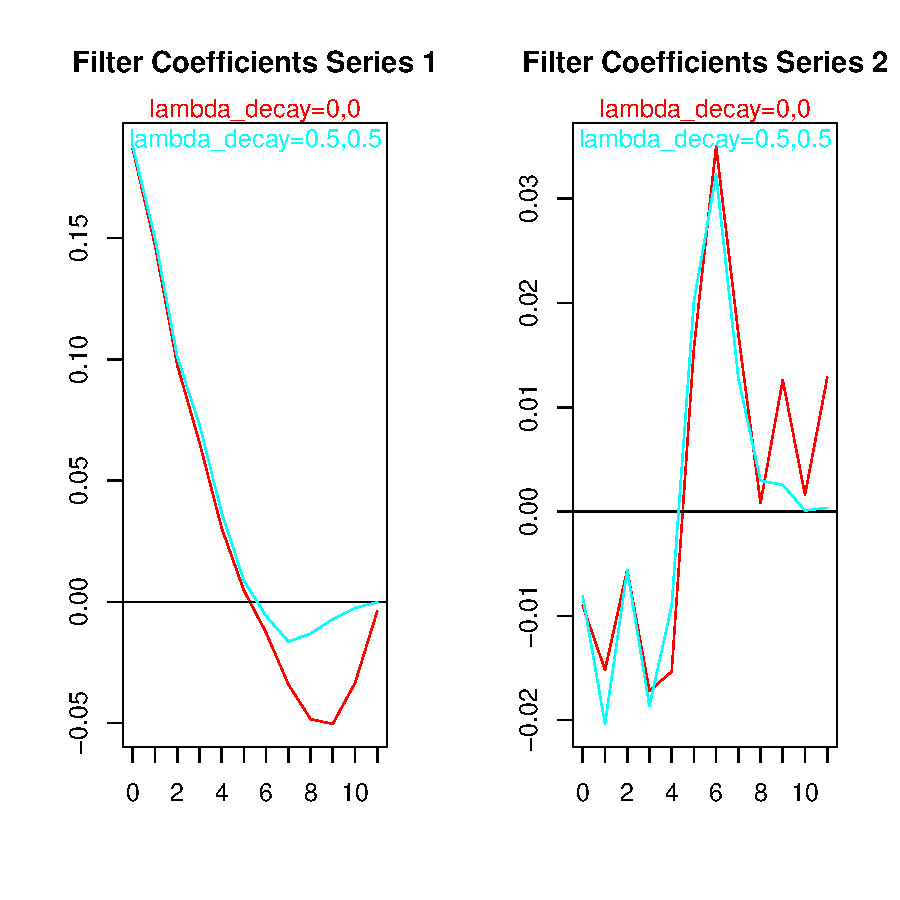
\includegraphics[height=3in, width=6in]{z_mdfa_ms_reg_decay}\caption{Filter Coefficients: original unregularized (red) vs. decay-regularization (cyan) for series 1 (left) and 2 (right) of the bivariate design, lambda-decay=(0.5,0.5)\label{z_mdfa_ms_reg_decay}}\end{center}\end{figure}As expected, the rate of decay of the regularized coefficients (cyan) is more pronounced. In order to measure the `effective' strength of the regularization we can compute the so-called \emph{effective degrees of freedom} of the estimates (see below for details): the regularization has shrunken the original unconstrained space, of dimension $24.09$ ($2*L$), to a subspace of (generally non-integer) dimension $16.66$: approximately ten degrees of freedom were lost by imposing the decay regularization and therefore in-sample and out-of-sample performances of the regularized design will be less incongruent (overfitting is tamed).



\subsection{Grid-Screening of Effects}

We here attempt to provide more insights into the decay-regularization by screening the specific effects controlled by $\lambda_{decay,1}$ and $\lambda_{decay,2}$.

\subsubsection{Shape-Parameter $\lambda_{decay,1}$}

 We first fix the strength-parameter $\lambda_{decay,2}:=0.5$ and compute estimates of the filter coefficients for a discrete grid of the shape-parameter $\lambda_{decay,1}=k\cdot 0.1$ with $k=-1,0,...,11$:  
\begin{Schunk}
\begin{Sinput}
> # Estimate filter coefficients: Decay-regularization
> lambda_decay_1<-0.5
> lambda_decay_2<-0.1*0:9
> lambda_decay_2<-c(lambda_decay_2,lambda_decay_2[length(lambda_decay_2)]+0.01*0:9,0.995,0.999,1)
\end{Sinput}
\end{Schunk}
The resulting filter-coefficients  are plotted in fig.\ref{z_mdfa_ms_reg_decay_screen_decay_1}: the effective degrees of freedom, $edof$, as well as the regularization settings are reported too.
\begin{Schunk}
\begin{Soutput}
RStudioGD 
        2 
\end{Soutput}
\end{Schunk}
\begin{figure}[H]\begin{center}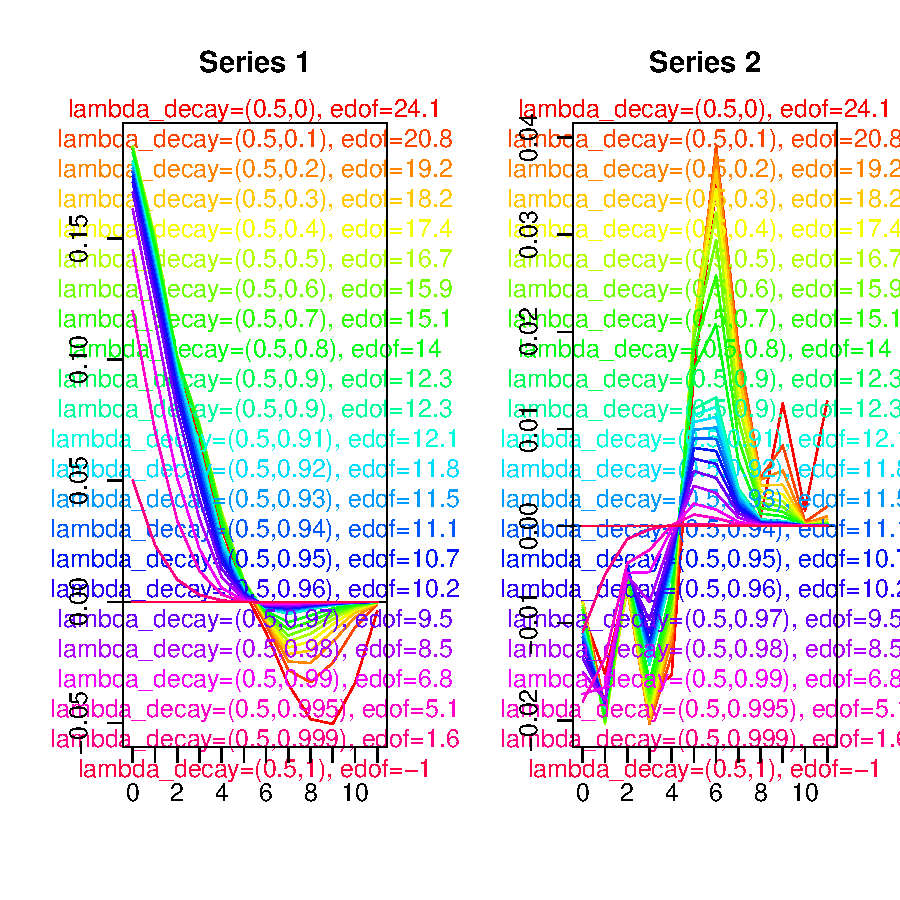
\includegraphics[height=4in, width=6in]{z_mdfa_ms_reg_decay_screen_decay_1}\caption{Filter Coefficients: effect of shape-parameter (grid of points -0.1, 0, 0.1, 0.2, ..., 1.1) for fixed strength parameter (0.5), series 1 (left) and 2 (right)\label{z_mdfa_ms_reg_decay_screen_decay_1}}\end{center}\end{figure}A small value of the shape-parameter $\lambda_{decay,1}$ implies that nearly equal weight is assigned to all coefficients, irrespective of the lag. In this case, the number of effective degrees of freedom, $edof$, is smallest and the overall shrinkage-effect is most pronounced. For increasing shape parameter, higher-lag coefficients are shrunken more heavily whereas small-lag coefficients get relaxed, in relative terms. Note that a larger shape-parameter $\lambda_{decay,1}$ tends, ceteris paribus, to enforce the strength of the regularization\footnote{This entanglement could be avoided by normalizing $\lambda_{decay,2}$ by $\frac{1}{L}\sum_{k=0}^{L-1}|1+\lambda_{decay,1}|^k$, for example (but we didn't).}. This effect explains the non-monotonicity of $edof$ as a function of $\lambda_{decay,1}$. Note, also, that the effect of $\lambda_{decay,1}$ is bounded to the interval $[0,1]$: our R-code relies on $\min(|\lambda_{decay,1}|,1)$, which explains why the estimates for $\lambda_{decay,1}=-0.1$ and $\lambda_{decay,1}=0.1$ (or for $\lambda_{decay,1}=1$ and $\lambda_{decay,1}=1.1$) are indistinguishable. \\


\subsubsection{Strength-Parameter $\lambda_{decay,2}$}


We now fix the shape-parameter $\lambda_{decay,1}=0.5$ and analyze effects by the strength-parameter $\lambda_{decay,2}=k\cdot 0.1$ where $k=-1,0,1,...,11$:
\begin{Schunk}
\begin{Sinput}
> # Estimate filter coefficients: Decay-regularization
> lambda_decay_1<-0.5
> lambda_decay_2<-0.1*-1:11
\end{Sinput}
\end{Schunk}
The resulting filter-coefficients  are plotted in fig.\ref{z_mdfa_ms_reg_decay_screen_decay_2}: the effective degrees of freedom, $edof$, as well as the regularization settings are reported too.
\begin{Schunk}
\begin{Soutput}
RStudioGD 
        2 
\end{Soutput}
\end{Schunk}
\begin{figure}[H]\begin{center}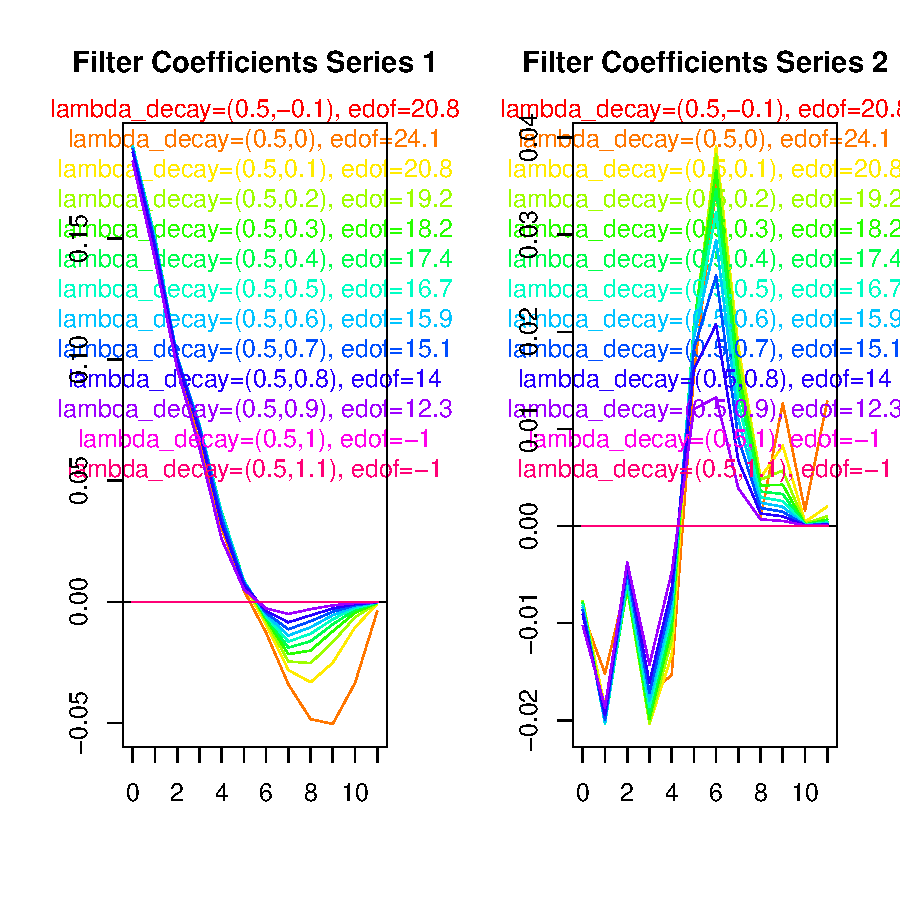
\includegraphics[height=4in, width=6in]{z_mdfa_ms_reg_decay_screen_decay_2}\caption{Filter Coefficients: effect of strength-parameter (grid of points -0.1,0, 0.1, 0.2, ..., 1.1) for fixed shape parameter (0.5), series 1 (left) and 2 (right)\label{z_mdfa_ms_reg_decay_screen_decay_2}}\end{center}\end{figure}The strength-parameter $\lambda_{decay,2}$ is bounded to the interval $[0,1]$, too (the code relies on $f(\min(|\lambda_{decay,2}|,1))$ where $f(\cdot)$ is a monotonic function with $f(0)=0$ and $f(1)=\infty$). If $\lambda_{decay,2}=0$ then no regularization is imposed and thus $edof=24.0946826274948$ ($=2L$). The number of effective degrees of freedom shrinks monotonically as a function of $\lambda_{decay,2}$: for `large' $\lambda_{decay,2}\to 1$, an asymptotically infinite weight\footnote{For numerical reasons we use a finite upper-bound in our R-code.} is obtained and therefore the coefficients are shrunken to zero i.e. $edof=0$ (the corresponding coefficients are confounded with the zero line).




\subsection{Constraints vs. Regularization}\label{con_vs_reg}


Hard-constraints, such as imposed by $i1$ or $i2$, see chapter \ref{con_sec}, are maintained irrespective of regularization settings: hard-constraints are prioritized and dominate the design. In the following example we compare unrestricted ($i1=i2=F$) and restricted filter estimates, whereby a simple level-constraint $i1=T$ is imposed in the latter case: $\hat{\Gamma}_1(0)=\hat{\Gamma}_2(0)=1$ (the transferfunctions of the two real-time filters of the bivariate design must equate one in frequency zero).


\begin{Schunk}
\begin{Sinput}
> # Estimate filter coefficients: Decay-regularization
> lambda_decay_1<-0.5
> lambda_decay_2<-c(0,0.5,1)
\end{Sinput}
\end{Schunk}
We now estimate coefficients for all four combinations of regularized/unregularized and constrained/unconstrained designs:
\begin{Schunk}
\begin{Sinput}
> # Source the default (MSE-) parameter settings
> source(file=paste(path.pgm,"control_default.r",sep=""))
> troikaner<-T
> # Unconstrained designs: with and without regularization
> b_mat_unrestricted<-matrix(nrow=L,ncol=(ncol(weight_func)-1)*length(lambda_decay_2))
> edof_vec_unrestricted<-rep(NA,length(lambda_decay_2))
> for (i in 1:length(lambda_decay_2))
+ {
+   lambda_decay<-c(lambda_decay_1,lambda_decay_2[i])
+   mdfa_obj_decay<-mdfa_analytic(L,lambda,weight_func,Lag,Gamma,eta,cutoff,i1,i2,weight_constraint,lambda_cross,lambda_decay,lambda_smooth,lin_eta,shift_constraint,grand_mean,b0_H0,c_eta,weight_structure,white_noise,synchronicity,lag_mat,troikaner)
+   b_mat_unrestricted[,(i-1)*(ncol(weight_func)-1)+1:(ncol(weight_func)-1)]<-mdfa_obj_decay$b
+   edof_vec_unrestricted[i]<-mdfa_obj_decay$degrees_freedom
+ }
> # Impose level-constraint
> i1<-T
> # Both transfer functions must equal one in frequency zero
> weight_constraint<-c(1,1)
> b_mat_restricted<-matrix(nrow=L,ncol=(ncol(weight_func)-1)*length(lambda_decay_2))
> edof_vec_restricted<-rep(NA,length(lambda_decay_2))
> for (i in 1:length(lambda_decay_2))
+ {
+   lambda_decay<-c(lambda_decay_1,lambda_decay_2[i])
+   mdfa_obj_decay<-mdfa_analytic(L,lambda,weight_func,Lag,Gamma,eta,cutoff,i1,i2,weight_constraint,lambda_cross,lambda_decay,lambda_smooth,lin_eta,shift_constraint,grand_mean,b0_H0,c_eta,weight_structure,white_noise,synchronicity,lag_mat,troikaner)
+   b_mat_restricted[,(i-1)*(ncol(weight_func)-1)+1:(ncol(weight_func)-1)]<-mdfa_obj_decay$b
+   edof_vec_restricted[i]<-mdfa_obj_decay$degrees_freedom
+ }
\end{Sinput}
\end{Schunk}
The resulting filter-coefficients  are plotted in fig.\ref{z_mdfa_ms_reg_decay_screen_decay_2_rest}: the effective degrees of freedom, $edof$, as well as the regularization settings are reported too.
\begin{Schunk}
\begin{Soutput}
RStudioGD 
        2 
\end{Soutput}
\end{Schunk}
\begin{figure}[H]\begin{center}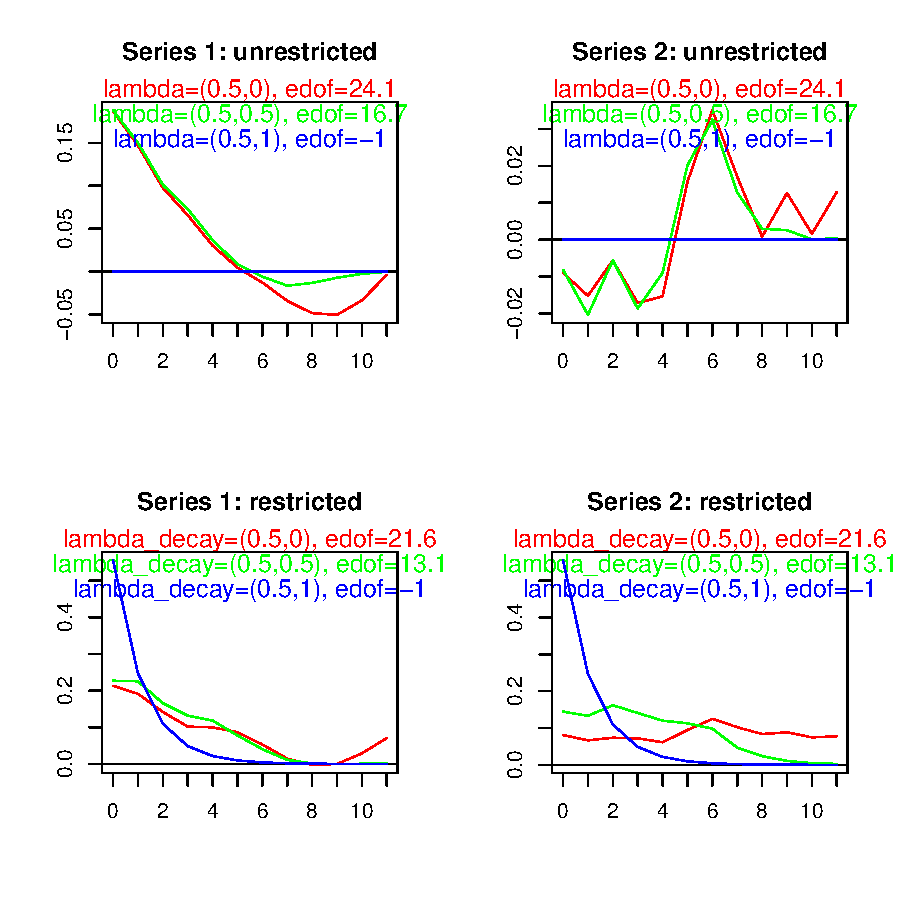
\includegraphics[height=6in, width=6in]{z_mdfa_ms_reg_decay_screen_decay_2_rest}\caption{Filter Coefficients: effect of constraints and strength-parameter (0, 0.5, 1) for fixed shape parameter (0.5), series 1 (left) and 2 (right); unconstrained design (top) vs. constrained design (bottom)\label{z_mdfa_ms_reg_decay_screen_decay_2_rest}}\end{center}\end{figure}Without regularization imposed (red lines), the constrained design (bottom) looses two degrees of freedom, dropping from $edof=24.1$ to $edof=21.6$. With full regularization imposed (blue lines) the unconstrained design (top) is shrunken to zero; in contrast the constrained design (bottom) must satisfy $\hat{\Gamma}_i(0)=\sum_{k=0}^{L-1}b_{ki}=1$ for $i=1,2$. Indeed, the latter constraints are satisfied by all filters, irrespective of regularization settings. To conclude, we note that level and time-shift constraints were parametrized in such a way that potential conflicts with the proposed regularization-term are avoided, irrespective of the lead (forecast) or lag (backcast) of the estimate, see section \ref{cons_gen_par}.









\section{Longitudinal Smoothness}


For each explaining time series $x_t$, $w_{it}$, $i=1,...,m$, in a real-time filter design, the corresponding filter coefficients $b_{ik}$\footnote{The case $i=0$ refers to the explaining data of $x_t$.}, for $i$ fixed, may be considered as functions of the lag $k=0,...,L-1$. A typical indication of overfitting is given when these lag-dependent functions are ragged i.e. when the series $b_{ik}$, for fixed $i$, are `noisy' or, more formally, when the curvatures (squared second order differences)
\begin{equation}\label{curvature_squa}
\sum_{k=0}^{L-3} \left((1-B)^2 b_{ik}\right)^2=\sum_{k=0}^{L-3}\left(b_{ik}-2b_{i,k+1}+b_{i,k+2}\right)^2
\end{equation}
are large.


\subsection{Quadratic Bilinear Form}


We may thus introduce a penalty-term whose bilinear form replicates \ref{curvature_squa}. Specifically, the regularized criterion becomes
\begin{eqnarray}\label{smooth_term}
MDFA+f(\lambda_{smooth})\mathbf{b}'\boldsymbol{\Lambda}_{smooth}^m\mathbf{b}\to \min_{\mathbf{b}}
\end{eqnarray}
where  $\boldsymbol{\Lambda}_{smooth}^m$ is a block-diagonal matrix of dimension $L(m+1)*L(m+1)$
\begin{eqnarray*}
\boldsymbol{\Lambda}_{smooth}^m=\left(\begin{array}{cccc}\boldsymbol{\Lambda}_{smooth}^0&0&...&0\\
                                              0&\boldsymbol{\Lambda}_{smooth}^0&...&0\\
                                              :::\\
                                              0&0&...&\boldsymbol{\Lambda}_{smooth}^0                                              
                                              \end{array}\right)
\end{eqnarray*}
with $L*L$-dimensional blocks $\boldsymbol{\Lambda}_{smooth}^0$
\begin{eqnarray*}
\boldsymbol{\Lambda}_{smooth}^0&=&\left(\begin{array}{ccccccccccccc}
1 &-2&1 &  0&0&0 &0&....&  &   &   &   &  0\\
-2& 5&-4&1 &0&0 &0&....&  &   &   &   &  0\\
1 &-4& 6&-4&1&0 &0&....&  &   &   &   &  0\\
0 &1 &-4& 6&-4&1&0&....&  &   &   &   &  0\\
::\\
0 & 0& 0&0&0 &0&...&1 &-4& 6&-4& 1& 0\\
0 &0 & 0& 0&0&0 &0&...&1 &-4& 6&-4& 1\\
0 &0 & 0& 0&0&0 &0&...&0 & 1 &-4& 5&-2\\
0 &0 & 0& 0&0&0 &0&...&0 & 0 &1 &-2&1  \\
\end{array}\right)
\end{eqnarray*}
The latter replicate the curvature measure \ref{curvature_squa} 
\[\sum_{k=0}^{L-3} \left((1-B)^2 b_{ik}\right)^2=\mathbf{b}_i'\boldsymbol{\Lambda}_{smooth}^0\mathbf{b}_i\]
for $i=0,...,m$\footnote{Checking this identity is graciously left as an exercise.}. In the univariate case we have $m=0$ and therefore $\boldsymbol{\Lambda}_{smooth}^m=\boldsymbol{\Lambda}_{smooth}^0$. As for the previous decay-regularization, $f(\lambda_{smooth})$ is a non-linear function of $\lambda_{smooth}$, with $f(0)=0, f(1)=\infty$, which measures the strength of the smoothness-regularization. If $\lambda_{smooth}=1$, then full regularization is imposed but, in contrast to the previous decay-term, the data is not completely discarded in this case, because shrinkage is applied to {second-order differences}. The proposed quadratic bilinear form is positive but not \emph{strictly} positive definite: its kernel consists of all functions which are linear in the lag $k$. Therefore, asymptotically, filter coefficients $b_{ik}$ must be linear, which still allows for multiple dependency from the data (such as scale and sign, for example). In particular the degrees of freedom shrink continuously from $L*(m+1)$ when $\lambda_{smooth}=0$ to $2*(m+1)$\footnote{Two parameters, namely intercept and slope, determine a linear function.} when $\lambda_{smooth}=1$. Note that the smoothness regularization is not affected by the lag parameter ($Lag$ or $-h$) and therefore the above mentioned applies indifferently to backcasting, nowcasting or forecasting, as well.



\subsection{Empirical Examples}

We rely on the above example and compute coefficients for a discrete grid $\lambda_{smooth}=k\cdot 0.1$, $k=-1,0,...,11$, of parameter values:  
\begin{Schunk}
\begin{Sinput}
> # Estimate filter coefficients: Decay-regularization
> #lambda_smooth_vec<-0.1*-1:11
> lambda_smooth_vec<-0.1*0:9
> lambda_smooth_vec<-c(lambda_smooth_vec,lambda_smooth_vec[length(lambda_smooth_vec)]+0.01*0:9,0.995,0.999,1)
\end{Sinput}
\end{Schunk}
The resulting filter-coefficients  are plotted in fig.\ref{z_mdfa_ms_reg_smooth_1}: the effective degrees of freedom, $edof$, as well as the accompanying regularization settings are reported too.
\begin{Schunk}
\begin{Soutput}
RStudioGD 
        2 
\end{Soutput}
\end{Schunk}
\begin{figure}[H]\begin{center}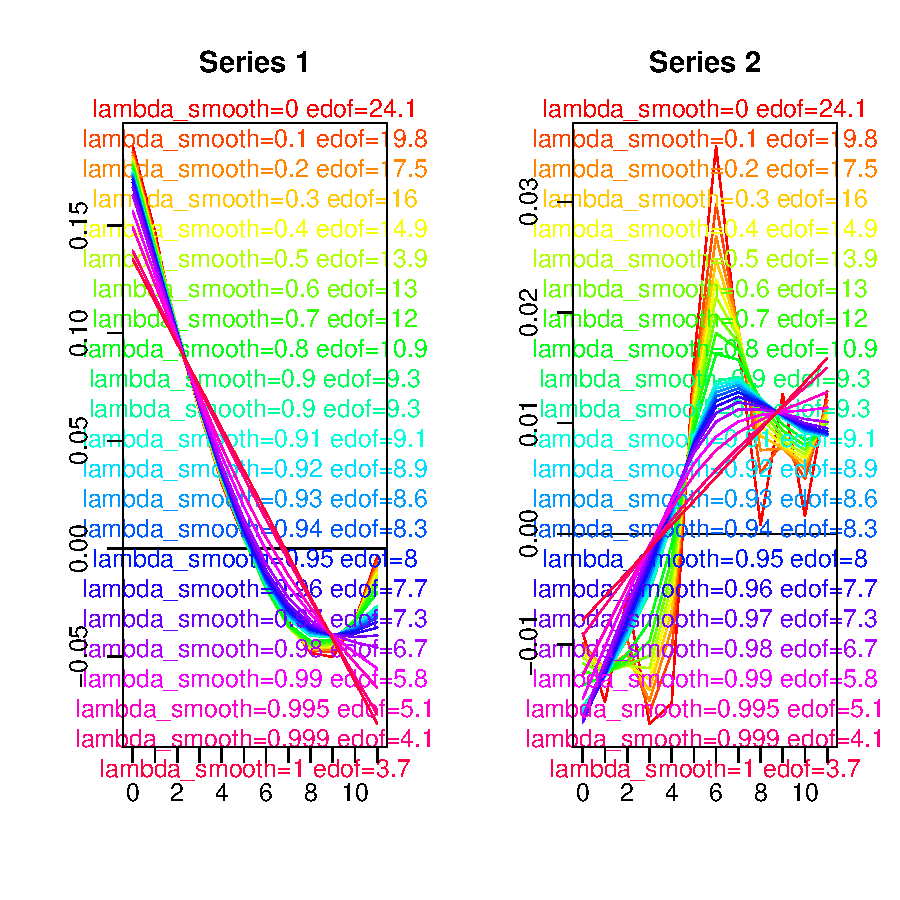
\includegraphics[height=4in, width=6in]{z_mdfa_ms_reg_smooth_1}\caption{Filter Coefficients: effect of smoothness regularization for grid-points -0.1, 0, 0.1, 0.2, ..., 1.1: series 1 (left) and 2 (right)\label{z_mdfa_ms_reg_smooth_1}}\end{center}\end{figure}The longitudinal smoothness of the filter coefficients is improved as $\lambda_{smooth}$ increases and the coefficients end-up as linear functions of the lag when full regularization is imposed. Unlike the previous decay-regularization, the coefficients are not shrunken towards zero for $\lambda_{smooth}=1$; in this case $edof=2*(m+1)=4$, as expected. In conformity with the previous decay-term, the effect of $\lambda_{smooth}$ is bounded to the interval $[0,1]$: our R-code relies on $f(\min(|\lambda_{decay,1}|,1))$ where $f(\cdot)$ is a monotonic function with $f(0)=0$ and $f(1)=\infty$. Therefore, the estimates for $\lambda_{smooth}=-0.1$ and $\lambda_{smooth}=0.1$ (or for $\lambda_{smooth}=1$ and $\lambda_{smooth}=1.1$) are identical.  



\section{Cross-Sectional Similarity}\label{cross_sec_sim}


Often, in practice, the time series $x_t,w_{it}$, $i=1,...,m$ of a multivariate design are redundant, at least to some extent\footnote{Business-cycles, for example, are defined as  pervasive co-movements across a range of interesting time series. In this context, it is not uncommon to assume that time series can be decomposed additively (eventually after suitable data-transformation) into a common generally non-stationary term (common factor) and a stationary idiosyncratic component (cointegration rank one). In such a case the common factor stands for the redundant information across the original data.}. In such a case it is not illegitimate to assume that filter coefficients should share common features, too: for example the rate of decay and/or the sign and/or the scale.

\subsection{Quadratic Bilinear Form}

In order to account for this possibility we here fix the lag-index $k$ and consider $b_{ik}$ as a function of the cross-sectional index $i=0,...,m$: for each (fixed) $k$, $b_{ik}$ should be similar or, stated otherwise, $b_{ik}$ should be close to the cross sectional mean $\frac{1}{m+1}\sum_{i=0}^mb_{ik}$\footnote{The cross-sectional means are the grand-means, see section \ref{gm_par}. However, our proceeding here avoids the undesirable asymmetry of the explicit grand-mean parametrization.}. Accordingly,  the penalty term amending additively the (M)DFA-criterion can be specified as
\begin{eqnarray}\label{centm}
\sum_{k=0}^{L-1}\sum_{i=0}^m\left(b_{ik}-\frac{1}{m+1}\sum_{i'=0}^mb_{i'k}\right)^2
\end{eqnarray}
Smaller values of this statistic signify enforced cross-sectional similarity of the coefficients, as desired. A suitable positive definite bilinear form replicating this penalty term is given by 
\begin{eqnarray}\label{sympa}
\boldsymbol{\Lambda}_{cross}^m&=&\mathbf{I}-\boldsymbol{M}
\end{eqnarray}
where $\mathbf{I}$ is an $L(m+1)*L(m+1)$-dimensional identity and
\begin{eqnarray*}
\boldsymbol{M}&=&\left(\begin{array}{ccc}\boldsymbol{\mu}&...&\boldsymbol{\mu}\\
:::\\
\boldsymbol{\mu}&...&\boldsymbol{\mu}\end{array}\right)
\end{eqnarray*}
is made of $(m+1)^2$ replications of the $L*L$-dimensional block $\boldsymbol{\mu}$
\begin{eqnarray*}
\boldsymbol{\mu}&=&\left(\begin{array}{cccc}
-\frac{1}{m+1}&0&...&0\\
0&-\frac{1}{m+1}&...&0\\
:::\\
0&0&...&-\frac{1}{m+1}
\end{array}\right)
\end{eqnarray*}
A juxtaposition of these blocks along the rows of $\boldsymbol{M}$ builds-up the cross-sectional means from the stacked (long) coefficient vector $\mathbf{b}=Vec(\mathbf{B})$. The corresponding regularized criterion becomes
\begin{eqnarray}\label{smooth_term}
MDFA+f(\lambda_{cross})\mathbf{b}'\boldsymbol{\Lambda}_{cross}^m\mathbf{b}\to \min_{\mathbf{b}}
\end{eqnarray}
where, once again, $f(\lambda_{cross})$ is a non-linear monotonic function with $f(0)=0, f(1)=\infty$. In the latter case, when full regularization is imposed, the cross-sectional differences are projected onto zero. As for the smoothness-term, the cross-sectional bilinear form is not strictly positive since its kernel is made of the common `grand-mean'. Asymptotically, the data still interacts with the regularized estimate: the remaining degrees of freedom shrink continuously from $(m+1)L$, when $\lambda_{cross}=0$, to $L$ when $\lambda_{cross}=1$.  Note that the cross-sectional regularization is not affected by the lag parameter ($Lag$ or $-h$) and therefore the above mentioned applies indifferently to backcasting, nowcasting or forecasting, as well.


\subsection{Empirical Examples}

We rely on the previous example and compute coefficients for a discrete grid $\lambda_{cross}=k\cdot 0.1$, $k=-1,0,...,11$, of parameter values:  
\begin{Schunk}
\begin{Sinput}
> # Estimate filter coefficients: Decay-regularization
> #lambda_cross_vec<-0.1*0:9
> lambda_cross_vec<-0.1*0:9
> lambda_cross_vec<-c(lambda_cross_vec,lambda_cross_vec[length(lambda_cross_vec)]+0.01*0:9,0.995,0.999,1)
\end{Sinput}
\end{Schunk}
The resulting filter-coefficients  are plotted in fig.\ref{z_mdfa_ms_reg_cross_1}: the effective degrees of freedom, $edof$, as well as the accompanying regularization settings are reported too.
\begin{Schunk}
\begin{Soutput}
RStudioGD 
        2 
\end{Soutput}
\end{Schunk}
\begin{figure}[H]\begin{center}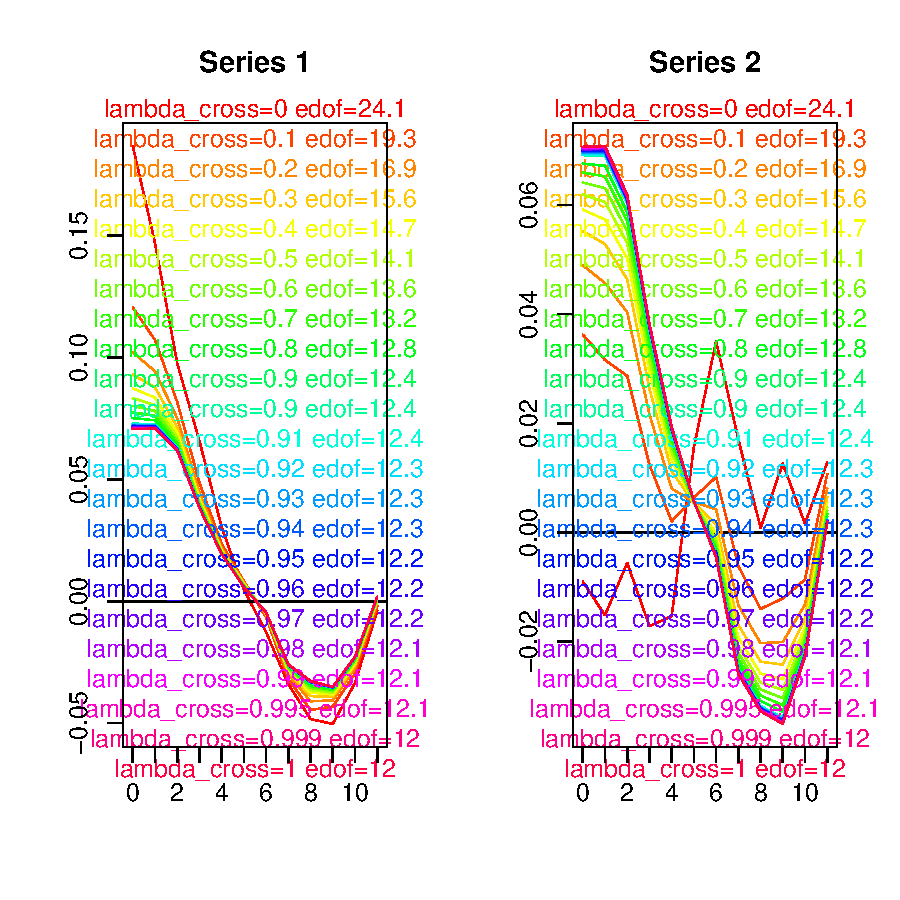
\includegraphics[height=4in, width=6in]{z_mdfa_ms_reg_cross_1}\caption{Filter Coefficients: effect of cross-sectional regularization for grid-points -0.1, 0, 0.1, 0.2, ..., 1.1: series 1 (left) and 2 (right)\label{z_mdfa_ms_reg_cross_1}}\end{center}\end{figure}For increasing $\lambda_{cross}$, filter coefficients for series 1 and 2 are merged more effectively, ending-up absorbed in the common  grand-mean, when full regularization is imposed (the coefficients in left and right panels are identical if $\lambda_{cross}\geq 1$). As for the smoothness-regularization, the coefficients are not shrunken towards zero for $\lambda_{cross}=1$; instead, the gap to the common grand-mean is closed and $edof=L (=12)$. In conformity with the previous regularization terms, the effect of $\lambda_{cross}$ is bounded to the interval $[0,1]$: our R-code relies on $f(\min(|\lambda_{cross,1}|,1))$ where $f(\cdot)$ is a monotonic function with $f(0)=0$ and $f(1)=\infty$. Therefore, the estimates for $\lambda_{cross}=-0.1$ and $\lambda_{cross}=0.1$ (or for $\lambda_{cross}=1$ and $\lambda_{cross}=1.1$) are identical. let us conclude here by emphasizing that the cross-sectional regularization is inadequate in the specific case of our toy-example because the second series of our bivariate design is independent from the target i.e. its coefficients should vanish\footnote{The common coefficients obtained for $\lambda_{cross}\geq 1$ in fig.\ref{z_mdfa_ms_reg_cross_1} are a shrunken version of the unregularized coefficients for series 1: whereas the first series is informative, the second-one just adds undesirable noise, which must be tamed by zero-shrinkage.}. 




\section{Regularization Troika: a Triplet of Universal Filter Requirements}\label{reg_troika_uni_req}

Instead of imposing possibly misspecified `hard' constraints, the proposed triplet of regularization-terms assigns `soft' preferences to particular sub-spaces of the ambient space $\mathbb{R}^{L(m+1)}$, which are felt to be of universal relevance. 

\subsection{Quadratic (Bilinear) Form}

An arbitrary combination and weighting of all three requirements can be obtained formally by the so-called Regularization Troika    
\begin{eqnarray}\label{troika}
MDFA+f(\lambda_{decay,2})\mathbf{b}'\boldsymbol{\Lambda}_{decay}^m\mathbf{b}+f(\lambda_{smooth})\mathbf{b}'\boldsymbol{\Lambda}_{smooth}^m\mathbf{b}+f(\lambda_{cross})\mathbf{b}'\boldsymbol{\Lambda}_{cross}^m\mathbf{b}\to \min_{\mathbf{b}}
\end{eqnarray}
If $\lambda_{decay,2}=\lambda_{smooth}=\lambda_{cross}=0$ then \ref{troika} replicates the original MDFA-criterion. Otherwise, degrees of freedom are shrunken by projecting filter coefficients onto sub-spaces which are \emph{un}likely to conflict with data (universality postulate) if the regularization is suitably balanced. Our credo --backed-up by experience -- is that the MDFA, endowed with the proposed regularization features, is able to tame overfitting without necessarily inflicting `misspecification' or statistical inefficiency: shrinkage-gains outweigh misspecification-losses such that, overall, out-of-sample performances improve.    



\subsection{Empirical Examples}

To be filled...


\subsection{Entanglement and Conflicting Requirements}

The proposed regularization features are not mutually orthogonal: as an example a strong decay-regularization may favor simultaneously smoothness  as well as cross-sectional similarity by attracting coefficients towards the `common' and `smooth' zero-line. Per contra, the  decay-regularization might also conflict with the smoothness requirement, since a rapid decay could be disruptive or discontinuous. It should be clear, therefore, that the regularization settings, as controlled by the hyperparameters $\boldsymbol{\lambda}_{decay}, \lambda_{smooth}$ and $\lambda_{cross}$ interact, either positively or negatively, to some extent. Interestingly, part of the conflicts can be resolved by specifying alternative origins of the shrinkage-spaces, see section \ref{h0_shrink}. Finally, let us remind here that regularization sub-spaces can be affected by imposing hard-constraints, see the example in section \ref{con_vs_reg}. 



\subsection{Limitations: Data Transformations}

Some of the proposed regularization features assume, at least implicitly, that the data is subject to specific homogeneity constraints. As a trivial example, the cross-sectional term assumes similarity of  time series in the data set (against the premicesses of our toy example). Filter-performances are no more invariant to (arbitrary) sign-changes or transformation of scales of time series if $\lambda_{cross}>0$. In a similar vein, the zero-shrinkage peculiar to the strictly positive definite decay-term assumes that the scales of the time series are identical or at least similar. Otherwise, the series with the smallest scale would be penalized more heavily because its coefficients are generally (though not always) larger, in absolute value. Performances are no more invariant to scale transformations if $\lambda_{decay,2}>0$. We therefore recommend to transform the data prior to regularization in such a way that the implicit homogeneity assumptions are met. In applications so far we found useful to match scales and signs of series\footnote{In order to measure performances in a consistent way, data transformations should always be causal i.e. they should not rely on future observations.}.         




\subsection{Empirical Examples}

To be filled...







\section{Optimization Criterion (Zero-Shrinkage)}\label{opt_crit_reg_tro}

We note that \ref{troika} is quadratic in the filter coefficients and therefore a unique closed-form solution exists. Using bilinear forms simplifies the derivation (as well as the notation) of the closed-form solution. We distinguish the cases of regularization with and without `hard' constraints (for example i1- and i2-constraints). 




\subsection{Unconstrained Design}\label{opt_reg_uncon}


Consider
\begin{eqnarray}\label{regcustreg}
&&(\mathbf{Y}^{\textrm{Cust}}(\eta)-\mathbf{X}^{\textrm{Cust}}(\lambda,\eta)\mathbf{b})'(\mathbf{Y}^{\textrm{Cust}}(\eta)-\mathbf{X}^{\textrm{Cust}}(\lambda,\eta)\mathbf{b})\nonumber\\
&+&\lambda_{{smooth}}\mathbf{b}'\boldsymbol{\Lambda}_{smooth}\mathbf{b}
+\lambda_{{cross}}\mathbf{b}'\boldsymbol{\Lambda}_{cross}\mathbf{b}+\lambda_{{decay,2}}\mathbf{b}'\boldsymbol{\Lambda}_{decay}\mathbf{b}\to\min
\end{eqnarray}
where $\mathbf{Y}^{\textrm{Cust}}(\eta)\in \mathbb{R}^{[T/2]+1}$ is a $[T/2]+1$-dimensional real-valued vector of dependent variables and where $\mathbf{X}^{\textrm{Cust}}(\lambda,\eta)\in \mathbb{C}^{([T/2]+1)(m+1)L}$ is a $([T/2]+1)*((m+1)L)$-dimensional complex-valued matrix of explaining data, see section \ref{l-scsmdfa}: for $\lambda=\eta=0$ no customization is imposed and therefore a classic MSE-estimate is obtained. Derivation of the criterion with respect to the stacked parameter vector $\mathbf{b}$ leads to
\begin{eqnarray*}
\frac{d}{d\mathbf{b}}~\textrm{Criterion}&=&\frac{d}{d\mathbf{b}}~(\mathbf{Y}^{\textrm{Cust}}(\eta)-\mathbf{X}^{\textrm{Cust}}(\lambda,\eta)\mathbf{b})'(\mathbf{Y}^{\textrm{Cust}}(\eta)-\mathbf{X}^{\textrm{Cust}}(\lambda,\eta)\mathbf{b})\nonumber\\
&+&\frac{d}{d\mathbf{b}}~\Big(\lambda_{{smooth}}\mathbf{b}'\boldsymbol{\Lambda}_{smooth}\mathbf{b}
+\lambda_{{cross}}\mathbf{b}'\boldsymbol{\Lambda}_{cross}\mathbf{b}+\lambda_{{decay,2}}\mathbf{b}'\boldsymbol{\Lambda}_{decay}\mathbf{b}\Big)\\
&=&-2\mathbf{Y}^{\textrm{Cust}}(\eta)'\Re\left(\mathbf{X}^{\textrm{Cust}}(\lambda,\eta)\right)+2\mathbf{b}'\Re\bigg\{\mathbf{X}^{\textrm{Cust}}(\lambda,\eta)'\mathbf{X}^{\textrm{Cust}}(\lambda,\eta)\bigg\}\\
&&+2\lambda_{{smooth}}\mathbf{b}'\boldsymbol{\Lambda}_{smooth}
+2\lambda_{{cross}}\mathbf{b}'\boldsymbol{\Lambda}_{cross}+2\lambda_{{decay},2}\mathbf{b}'\boldsymbol{\Lambda}_{decay}
\end{eqnarray*}
where we used the fact that the proposed bilinear forms are symmetric. Equating this expression to zero, the generalized regularized solution is obtained as
\begin{eqnarray}\label{bregcustreg}
&&\mathbf{\hat{b}}^{\textrm{Cust-Reg}}(\lambda,\eta,\lambda_{{smooth}},\lambda_{{cross}},\lambda_{{decay,1}},\lambda_{decay,2})=\\
&&\left(\Re\bigg\{\mathbf{X}^{\textrm{Cust}}(\lambda,\eta)' \mathbf{X}^{\textrm{Cust}}(\lambda,\eta)\bigg\}+
\lambda_{{smooth}}\boldsymbol{\Lambda}_{smooth}+\lambda_{{cross}}\boldsymbol{\Lambda}_{cross}+\lambda_{{decay},2}\boldsymbol{\Lambda}_{decay}
\right)^{-1}\nonumber\\
&&\Re(\mathbf{X}^{\textrm{Cust}}(\lambda,\eta))'
\mathbf{Y}^{\textrm{Cust}}(\eta)\nonumber
\end{eqnarray}
As can be seen, each term of the Regularization Troika contributes in `regularizing' the matrix subject to inversion: ill-posed problems with $L$ large (large filter order) and/or $m$ large (high-dimensional design) can be solved effectively by imposing suitable shrinkage towards idealized filter patterns. In particular, the number $(m+1)L$ of unknown filter coefficients may exceed the sample size $T$\footnote{This would allow for a formal treatment of high-dimensional designs ($m$ large), for example.}.  



\subsection{Constrained Design}

We assume that the filter constraints can be written in the form
\begin{eqnarray}\label{cons5s}
\mathbf{b}&=&\mathbf{R}(i1,i2) \mathbf{b_{f}}+\mathbf{c}(i1,i2)
\end{eqnarray}
where $\mathbf{b_f}$ is the vector of freely determined coefficients and where $\mathbf{R}(i1,i2)$ and $\mathbf{c}(i1,i2)$ depend on the booleans $i1,i2$, see section \ref{matrix_notation_constraints} (alternative constraints could be considered, of course). Plugging this expression into \ref{regcustreg} and taking derivatives with respect to the stacked vector of freely determined coefficients $\mathbf{b_{f}}$, we obtain (note that the functional dependencies of $\mathbf{Y}^{\textrm{Cust}}(\eta), \mathbf{X}^{\textrm{Cust}}(\lambda,\eta)$ on the customization parameters $\lambda,\eta$ are omitted for notational simplicity):
\begin{eqnarray*}
\frac{d}{d\mathbf{b_f}}~\textrm{Criterion}&=&\frac{d}{d\mathbf{b_f}}~(\mathbf{Y}^{\textrm{Cust}}-\mathbf{X}^{\textrm{Cust}}\left(\mathbf{R b_{f}+c}\right))'(\mathbf{Y}^{\textrm{Cust}}-\mathbf{X}^{\textrm{Cust}}\left(\mathbf{R b_{f}+c}\right))\nonumber\\
&+&\frac{d}{d\mathbf{b_f}}~\lambda_{{smooth}}\left(\mathbf{R b_{f}+c}\right)'\boldsymbol{\Lambda}_{smooth}\left(\mathbf{R b_{f}+c}\right)\\
&+&\frac{d}{d\mathbf{b_f}}~\lambda_{{cross}}\left(\mathbf{R b_{f}+c}\right)'\boldsymbol{\Lambda}_{cross}\left(\mathbf{R b_{f}+c}\right)\\
&+&\frac{d}{d\mathbf{b_f}}~\lambda_{{decay},2}\left(\mathbf{R b_{f}+c}\right)'\boldsymbol{\Lambda}_{decay}\left(\mathbf{R b_{f}+c}\right)\\
&=&-2(\mathbf{Y}^{\textrm{Cust}})'\Re\left(\mathbf{X}^{\textrm{Cust}}\right)\mathbf{R}+
2\Re\bigg\{\mathbf{(X^{\textrm{Cust}}c)'(X^{\textrm{Cust}}R)}\bigg\}
+2\mathbf{b}_f'\Re\bigg\{(\mathbf{X}^{\textrm{Cust}}\mathbf{R})'\mathbf{X}^{\textrm{Cust}}\mathbf{R}\bigg\}\\
&&+2\lambda_{{smooth}}\mathbf{b_f'R'}\boldsymbol{\Lambda}_{smooth}\mathbf{R}+2\lambda_{{smooth}}\mathbf{(c'}\boldsymbol{\Lambda}_{{smooth}}\mathbf{R)}\\
&&+2\lambda_{{cross}}\mathbf{b_f'R'}\boldsymbol{\Lambda}_{cross}\mathbf{R}+2\lambda_{{cross}}\mathbf{(c'}\boldsymbol{\Lambda}_{{cross}}\mathbf{R)}\\
&&+2\lambda_{{decay},2}\mathbf{b_f'R'}\boldsymbol{\Lambda}_{decay}\mathbf{R}+2\lambda_{{decay},2}\mathbf{(c'}\boldsymbol{\Lambda}_{\textrm{decay}}\mathbf{R)}
\end{eqnarray*}
where, again, we used the fact that the proposed bilinear forms are symmetric. Equating this expression to zero, the \emph{customized, regularized and constrained }solution is obtained as
\begin{eqnarray}\label{bregcustregconst}
&&\mathbf{\hat{b}}^{\textrm{Cust-Reg-Const}}_f(\lambda,\eta,\lambda_{{smooth}},\lambda_{{cross}},\lambda_{{decay},1},\lambda_{{decay},2},i1,i2)\nonumber\\
&=&\Big\{\Re\Big[(\mathbf{X}^{\textrm{Cust}}\mathbf{R})' \mathbf{X}^{\textrm{Cust}}\mathbf{R}\Big]+
\lambda_{{smooth}}\mathbf{R}'\boldsymbol{\Lambda}_{smooth}\mathbf{R}+\lambda_{{cross}}\mathbf{R}'\boldsymbol{\Lambda}_{cross}\mathbf{R}+\lambda_{{decay},2}\mathbf{R}'\boldsymbol{\Lambda}_{decay}\mathbf{R}
\Big\}^{-1}\nonumber\\
&&\Big((\Re(\mathbf{X^{\textrm{Cust}})R})'
\mathbf{Y}^{\textrm{Cust}}-\Re\bigg\{(\mathbf{X^{\textrm{Cust}}R})'\mathbf{X^{\textrm{Cust}}c}\bigg\}-
\mathbf{R}'(\lambda_{{smooth}}\boldsymbol{\Lambda}_{\textrm{smooth}}+\lambda_{{cross}}\boldsymbol{\Lambda}_{{cross}}+
\lambda_{{decay},2}\boldsymbol{\Lambda}_{{cross}})\mathbf{c}\Big)\nonumber\\
&=&\Big\{\Re\Big[\mathbf{R}'(\mathbf{X}^{\textrm{Cust} })' \mathbf{X}^{\textrm{Cust}}\mathbf{R}\Big]+
\lambda_{{smooth}}\mathbf{R}'\boldsymbol{\Lambda}_{{smooth}}\mathbf{R}+\lambda_{{cross}}\mathbf{R}'\boldsymbol{\Lambda}_{cross}\mathbf{R}+\lambda_{{decay},2}\mathbf{R}'\boldsymbol{\Lambda}_{decay}\mathbf{R}
\Big\}^{-1}\nonumber\\
&&\Big((\Re(\mathbf{X}^{\textrm{Cust}})\mathbf{R})'
\mathbf{Y}^{\textrm{Cust}}+\mathbf{Const}\Big)
\end{eqnarray}
where 
\begin{eqnarray*}
\mathbf{Const}=-\mathbf{R}'\Big\{\Re\Big[(\mathbf{X}^{\textrm{Cust}})'\mathbf{X}^{\textrm{Cust}}\Big]+
\lambda_{{smooth}}\boldsymbol{\Lambda}_{{smooth}}+\lambda_{{cross}}\boldsymbol{\Lambda}_{{cross}}+
\lambda_{{decay},2}\boldsymbol{\Lambda}_{{decay}}\Big\}\mathbf{c}
\end{eqnarray*}
This last term collects all level constraints\footnote{Indeed, $\mathbf{c=0}$ if $i1=F$.}. A comparison with \ref{bregcustreg} illustrates that both expressions - with or without constraints - are formally quite similar, up to the additional transformation by $\mathbf{R}$ and the emergence of a new generalized level-shift $\mathbf{Const}$: setting $\mathbf{R=Id}$ and $\mathbf{c=0}$ (no constraints involved) in the above solution indeed replicates  \ref{bregcustreg}. The result of the optimization is $\mathbf{b_f}$, the vector of freely determined coefficients. 
The sought-after `full-coefficient' vector $\mathbf{b}$, which is indispensable for the filtering-task, is then obtained from \ref{cons5s}.\\


\subsection{Empirical Example: Constrained Regularized Customized Design}

To be filled...


\section{Effective Degrees of $\textrm{Freedom}^*$}\label{reg_tr_eff_deg_free}

In the absence of regularization, the number of effective degrees of freedom $edof$ coincides with the number of freely determined filter coefficients (the length of the stacked vector $\mathbf{b_f}$); otherwise, $edof$ is reduced. We here derive a statistic which extends  $edof$ to the generic Regularization Troika. In contrast to the classic (real-valued) linear regression framework, the MDFA-criterion is subject to technical  peculiarities because the filter coefficients, as determined in a complex-valued space (frequency-domain), are required to be real-valued. As a result, the hat-matrix is neither symmetric, nor a projection anymore. As we shall see, this problem can be overcome by introducing a so-called adjoined imaginary estimate (the purely imaginary least-squares solution) and by augmenting the original hat-matrix by the resulting adjoined hat-matrix. For technically-averse readers, the results in this section can be skipped without impairing comprehension of later topics. %Determining a meaningful statistic for inferring this number in the presence of regularization is a non-trivial task and, moreover, a potentially equivocal prospect since multiple definitions are provided in the literature\footnote{A quick-and-dirty review is proposed in ????. These definitions are equivalent in the absence of regularization but they differ otherwise because the hat-matrix (to be defined below) is no more a projection, in general.}. However, a unique pertinent definition can be obtained when aiming at an explicit control of overfitting. For that purpose we address the \emph{spurious} decrease of the empirical  mean-square filter error or, equivalently, the spurious decrease of the criterion value as a function of the number of filter coefficients\footnote{Our approach is similar, in spirit, to ???, though not identical.}. In analogy to the previous section we distinguish unconstrained and constrained designs. 


\subsection{Hat-Matrix and Residual-Matrix}

For simplicity of exposition we here treat the unconstrained case as obtained by criterion \ref{regcustreg}.
The so-called \emph{hat-matrix} $\mathbf{H}$ is defined by 
\begin{eqnarray}
\mathbf{H}&=&\mathbf{X}^{\textrm{Cust}}\left(\Re\big\{(\mathbf{X}^{\textrm{Cust}})' \mathbf{X}^{\textrm{Cust}}\big\}+
\lambda_{{smooth}}\boldsymbol{\Lambda}_{smooth}+\lambda_{{cross}}\boldsymbol{\Lambda}_{cross}+\lambda_{{decay},2}\boldsymbol{\Lambda}_{decay}
\right)^{-1}\Re(\mathbf{X}^{\textrm{Cust}})'\label{hat_matrix_ex}
\end{eqnarray}
Thus
\[\mathbf{\hat{Y}^{\textrm{Cust}}:={X}^{\textrm{Cust}}\hat{b}}=\mathbf{HY^{\textrm{Cust}}}\]
i.e. $\mathbf{H}$ maps the dependent variable $\mathbf{Y}$ onto $\mathbf{\hat{Y}^{\textrm{Cust}}}$. In the absence of regularization, the expression for $\mathbf{H}$ simplifies to
\begin{eqnarray*}
\mathbf{H}&=&\mathbf{X}^{\textrm{Cust}}\left(\Re\big\{(\mathbf{X}^{\textrm{Cust}})' \mathbf{X}^{\textrm{Cust}}\big\}
\right)^{-1}\Re(\mathbf{X}^{\textrm{Cust}})'
\end{eqnarray*}
Note that $\mathbf{\hat{Y}^{\textrm{Cust}}}$  lies in a particular subspace of the complex plane spanned by the data $\mathbf{X}^{\textrm{Cust}}$, determined by the requirement that the least-squares solution must be real-valued\footnote{If we relaxed this restriction, i.e. if we allowed for an unrestricted complex-valued least-squares solution, then the resulting hat-matrix would be
\[\mathbf{H}=\mathbf{X}^{\textrm{Cust}}\left((\mathbf{X}^{\textrm{Cust}})' \mathbf{X}^{\textrm{Cust}}\right)^{-1}(\mathbf{X}^{\textrm{Cust}})'\]
This matrix would be a symmetric (hermitian) projection with eigenvalues either one or zero.}. Therefore, the complex-valued hat-matrix $\mathbf{H}$ is generally asymmetric ($\mathbf{H}\neq \mathbf{H}'$) and it is no more a projection since 
\begin{eqnarray*}
\mathbf{H'H}&=&\mathbf{\overline{H}^TH}\\
&=&\Re(\mathbf{X}^{\textrm{Cust}})\left(\Re\big\{(\mathbf{X}^{\textrm{Cust}})' \mathbf{X}^{\textrm{Cust}}\big\}
\right)^{-1}(\mathbf{X}^{\textrm{Cust}})'\mathbf{X}^{\textrm{Cust}}\left(\Re\big\{(\mathbf{X}^{\textrm{Cust}})' \mathbf{X}^{\textrm{Cust}}\big\}
\right)^{-1}\Re(\mathbf{X}^{\textrm{Cust}})\\
&\neq& \mathbf{H}
\end{eqnarray*}
Interestingly, though, an idempotency is obtained when focusing on the real-parts only:
\begin{eqnarray*}
\Re\left(\mathbf{H'H}\right)&=&\Re(\mathbf{X}^{\textrm{Cust}})\left(\Re\big\{(\mathbf{X}^{\textrm{Cust}})' \mathbf{X}^{\textrm{Cust}}\big\}
\right)^{-1}\Re\Big((\mathbf{X}^{\textrm{Cust}})'\mathbf{X}^{\textrm{Cust}}\Big)\left(\Re\big\{(\mathbf{X}^{\textrm{Cust}})' \mathbf{X}^{\textrm{Cust}}\big\}
\right)^{-1}\Re(\mathbf{X}^{\textrm{Cust}})\\
&=&\Re(\mathbf{X}^{\textrm{Cust}})\left(\Re\big\{(\mathbf{X}^{\textrm{Cust}})' \mathbf{X}^{\textrm{Cust}}\big\}
\right)^{-1}\Re(\mathbf{X}^{\textrm{Cust}}) \\
&=&\Re(\mathbf{H})
\end{eqnarray*}
Also, in contrast to the classic linear regression framework, the eigenvalues of $\mathbf{H}$ are not restricted to unity or zero: they are generally complex-valued and can be larger or smaller than one, in absolute value. Finally, the trace of the hat-matrix does not correspond to the effective degrees of freedom, anymore
\[tr(\mathbf{H})\neq (m+1)L\]
In fact, $tr(\mathbf{H})$ is a (data-dependent) random-variable. \\

The \emph{residual-matrix} $\mathbf{Res}$ is defined by
\[\mathbf{Res:=I-H}\]
It maps the dependent variable $\mathbf{Y}$ onto the filter error $\mathbf{(I-H)Y}=\mathbf{Y}-\hat{\mathbf{Y}}$. In analogy to the former hat-matrix, the latter residual-matrix  is no more symmetric, it is no more a projection and its trace is a (data-dependent) random-variable. Interestingly, though, 
\begin{eqnarray*}
\Re\left(\mathbf{(I-H)'\hat{Y}}\right)&=&\Re\left(\mathbf{(I-H)'HY}\right)\\
&=&\left(\Re(\mathbf{H})-\Re(\mathbf{H'H})\right)\mathbf{Y}\\
&=&\mathbf{0}
\end{eqnarray*}
i.e. the residual-matrix retains orthogonality, at least for real parts. 
We now propose an extension of these (classic) concepts which allow for a formal and general definition of the number of effective degrees of freedom $edof$ in the generic MDFA-framework. 




\subsection{A Generalization of $edof$: Adjoined Complex Estimate and Symmetric Augmentation of the Hat-Matrix}

The origin of the above difficulties resides in the asymmetry of the hat-matrix $\mathbf{H}$ which is imputable to its imaginary part. Fundamentally, this asymmetry is caused by requiring the least-squares coefficient-vector $\hat{\mathbf{b}}$ to be real-valued. Consider now the following (asymmetric) optimization problem
\begin{eqnarray*}
&&(\mathbf{Y}^{\textrm{Cust}}(\eta)-\mathbf{X}^{\textrm{Cust}}(\lambda,\eta)i\mathbf{b})'(\mathbf{Y}^{\textrm{Cust}}(\eta)-\mathbf{X}^{\textrm{Cust}}(\lambda,\eta)i\mathbf{b})\\
&=&\left|\mathbf{Y}^{\textrm{Cust}}(\eta)-\mathbf{X}^{\textrm{Cust}}(\lambda,\eta)i\mathbf{b}\right|^2\\
&=&\left|-i\mathbf{Y}^{\textrm{Cust}}(\eta)-\mathbf{X}^{\textrm{Cust}}(\lambda,\eta)\mathbf{b}\right|^2
\end{eqnarray*}
where $i\mathbf{b}$ is supposed to be purely imaginary. The last equation suggests that we may be looking for a purely real solution $\mathbf{b}$ after rotating the (real-valued) target by $\pi/2$, from $\mathbf{Y}^{\textrm{Cust}}(\eta)$ to $-i\mathbf{Y}^{\textrm{Cust}}(\eta)$. We name this problem \emph{adjoined  optimization criterion} and  the resulting purely imaginary (least-squares) solution is called \emph{adjoined estimate}. Its closed-form is obtained from
\begin{eqnarray*}
d/d\mathbf{b}~\textrm{Adjoined Criterion}&=&d/d\mathbf{b}~ (-i\mathbf{Y^{\textrm{Cust}}-X^{\textrm{Cust}}b})'(-i\mathbf{Y^{\textrm{Cust}}-X^{\textrm{Cust}}b})\\
&=&-(-i\mathbf{Y}^{\textrm{Cust}}-\mathbf{X^{\textrm{Cust}}b})'\mathbf{X^{\textrm{Cust}}}-(-i\mathbf{Y}^{\textrm{Cust}}-\mathbf{X^{\textrm{Cust}}b)^T\overline{X^{\textrm{Cust}}}}\nonumber\\
&=&2\mathbf{Y^{\textrm{Cust}}}'\Im\left(\mathbf{X^{\textrm{Cust}}}\right)+2\mathbf{b}'\mathbf{\Re((X^{\textrm{Cust}})'X^{\textrm{Cust}})}\nonumber
\end{eqnarray*}
where we used the fact that $(i\mathbf{Y}^{\textrm{Cust}})'=-i(\mathbf{Y}^{\textrm{Cust}})'$, since $\mathbf{Y}^{\textrm{Cust}}$ is real-valued. We deduce that the adjoined (purely imaginary) least-squares estimate $\mathbf{\hat{b}}^{ad}$ is obtained as
\begin{eqnarray*}
\mathbf{\hat{b}}^{ad}&=&-i\mathbf{\left(\Re((X^{\textrm{Cust}})'X^{\textrm{Cust}})\right)^{-1}}\mathbf{\Im\left(X^{\textrm{Cust}}\right)'Y^{\textrm{Cust}}}\\
&=&i\mathbf{\left(\Re((X^{\textrm{Cust}})'X^{\textrm{Cust}})\right)^{-1}}\mathbf{\Im\left((X^{\textrm{Cust}})'\right)Y^{\textrm{Cust}}}
\end{eqnarray*}
where the last equality follows from $\mathbf{\Im\left(X^{\textrm{Cust}}\right)'}=-\mathbf{\Im\left((X^{\textrm{Cust}})'\right)}$. 
The corresponding adjoined hat-matrix $\mathbf{H}^{ad}$ is
\begin{eqnarray*}
\mathbf{H}^{ad}=i\mathbf{X^{\textrm{Cust}}}\mathbf{\left(\Re((X^{\textrm{Cust}})'X^{\textrm{Cust}})\right)^{-1}}\mathbf{\Im\left((X^{\textrm{Cust}})'\right)}
\end{eqnarray*}
Let us now define the \emph{augmented hat-matrix} $\mathbf{H}^{aug}$ as the sum of original and adjoined hat-matrices
\begin{eqnarray*}
\mathbf{H}^{aug}&=&\mathbf{H}+\mathbf{H}^{ad}\\
&=&\mathbf{X^{\textrm{Cust}}}\mathbf{\left(\Re((X^{\textrm{Cust}})'X^{\textrm{Cust}})\right)^{-1}}\mathbf{\left(X^{\textrm{Cust}}\right)'}
\end{eqnarray*}
From the last equality we infer that the augmented hat-matrix is symmetric\footnote{Note however that it is not a projection.} $\mathbf{H}^{aug}=(\mathbf{H}^{aug})'$ and therefore its diagonal must be real-valued\footnote{Recall that $(\mathbf{H}^{aug})'=\overline{\mathbf{H}^{aug}}^T$ is the hermitian conjugate.}. We then obtain 
\begin{eqnarray*}
tr(\mathbf{H}^{aug})&=&tr\left(\mathbf{X}^{\textrm{Cust}}\left(\Re\big\{(\mathbf{X}^{\textrm{Cust}})' \mathbf{X}^{\textrm{Cust}}\big\}
\right)^{-1}(\mathbf{X}^{\textrm{Cust}})'\right)\\
&=&tr\left((\mathbf{X}^{\textrm{Cust}})'\mathbf{X}^{\textrm{Cust}}\left(\Re\big\{(\mathbf{X}^{\textrm{Cust}})' \mathbf{X}^{\textrm{Cust}}\big\}\right)^{-1}\right)\\
&=&tr\left(\Re\Big\{(\mathbf{X}^{\textrm{Cust}})'\mathbf{X}^{\textrm{Cust}}\Big\}\left(\Re\big\{(\mathbf{X}^{\textrm{Cust}})' \mathbf{X}^{\textrm{Cust}}\big\}\right)^{-1}\right)\\
&=&tr(\mathbf{I}_{(m+1)L})\\
&=&(m+1)L
\end{eqnarray*}
where the third equality is a consequence of the trace being real and linear and where $\mathbf{I}_{(m+1)L}$ is an $(m+1)L*(m+1)L$-dimensional identity. Since the trace of the augmented hat-matrix $\mathbf{H}^{aug}$ is a fixed number (not a random variable depending on the data) coinciding with $edof=(m+1)L$\footnote{It is assumed that the data is of full rank.} in the absence of regularization, we are now in a position to extend the concept of the effective degrees of freedom to the case of arbitrary regularization by defining
\begin{eqnarray*}
edof(\boldsymbol{\lambda}_{decay},\lambda_{smooth},\lambda_{cross}):=tr(\mathbf{H}^{aug}(\boldsymbol{\lambda}_{decay},\lambda_{smooth},\lambda_{cross}))
\end{eqnarray*}
where the augmented hat-matrix $\mathbf{H}^{aug}(\cdot)$ is now considered as a function of the general regularization settings. This number has been reported in the previous figures: in the presence of regularization it is generally non-integer valued. To conclude, note that the constrained and regularized optimization criterion \ref{bregcustregconst} can be tackled analogously and does not deserve a separate treatment here.





\subsection{Empirical Examples}

To be filled












\section{The Troikaner}

To be filled...

\subsection{Generalized Information Criterion}



\section{General H0-Shrinkage}\label{h0_shrink}

To be filled...

\subsection{Zero-Shrinkage vs. Regularization: Potentially Conflicting Requirements}


\subsection{Inclusion of A Priori Knowledge}


\subsection{Replicating (and Enhancing) Clients' Performances}

\section{Optimization Criterion under General H0-Shrinkage}

To be filled...


\section{MDFA-Stages}

To be filled...

\begin{itemize}
\item Numerically (very) fast
\item Statistically efficient
\item Immunized against Overfitting
\item Highly Adaptive
\end{itemize}



\section{Unsmoothing}

Difficult task: heavy smoothing. It requires long filters which are prone to overfitting (if not regularized). Idea:
\begin{itemize}
\item Apply a very simple (univariate) 0-stage filter which oversmooths the data (for example equally weighted or white noise DFA with very small cutoff)
\item At the first MDFA-stage apply a filter of length 2 or 3 with 0-shrinkage, based on the multivariate DFT, whose purposes are
\begin{itemize}
\item Account for sign (unemployment vs- production)
\item Account for scale (if series are not standardized)
\item Account for time-shift by unsmoothing the stage 0 filter (L>=2 allows for difference-like designs which unsmooth the filtered data and provide an anticipation)
\end{itemize}
\item Statistically efficient
\item Immunized against Overfitting
\item Highly Adaptive
\end{itemize}



\section{Summary}

\begin{itemize}
\item Overfitting is an unavoidable and direct consequence of determining filter coefficients according to an optimization principle: the perfected in-sample fit systematically understates the difficulty of the estimation problem. 
\item The transition from in-sample to out-of-sample performances  is generally smooth and gradual in signal-extraction problems (in contrast to classic one-step ahead forecasting) and the transition depends on the rate of decay of the coefficients $\gamma_k$ of the target.  
\item Improving out-of-sample performances by taming overfitting is an imbalancing act, whereby shrinkage-gains must outweigh misspecification-losses.
\item The Regularization Troika complies with this view by assigning soft preferences to sub-spaces which are felt to be of universal relevance in terms of longitudinal decay, longitudinal smoothness and cross-sectional similarity of filter coefficients. If these characteristics are shared by the truly best (but unobserved) coefficients, then shrinkage does not conflict with efficiency.
\item Finding optimal regularization weights $\boldsymbol{\lambda}_{decay},\lambda_{smooth}, \lambda_{cross}$ is a balancing act whose outcome strongly depends on user-preferences (utility function\footnote{As a factual example, mean-square performances and trading performances are incongruent to a large extent, due to scale-invariance, anisotropy and non-linearity effects.}). 
\item The solution of the regularized quadratic criterion can be obtained in closed form. 
\item An expression for the effective degrees of freedom of a regularized filter can be derived by augmenting the original hat-matrix, corresponding to the purely real-valued least-squares solution, by the adjoined hat-matrix, corresponding to the purely imaginary least-squares solution.
\end{itemize}

%----------------------------------------








\chapter{Vintage Data: Working with Data-Revisions}
%\label{rev_sec}
\label{vintages_triangle_revision}
\label{fil_sec}

refer to 2011-paper
\section{Introduction}

\section{Data Organization}

\subsection{Vintage and Release Triangles}

\subsection{Vintage Triangle in the Frequency-Domain}


\section{Reconcile Real-Time Signalextraction and Data-Revisions}

\subsection{Vintage-Filtering/Smoothing}

\subsection{Setting-Up MDFA-Designs: the (Pseudo-) Stationary Case}

\subsection{Extension to Non-Stationary Time Series}\label{rev_sec_int}

Refer and link to section \ref{coint_sec}

%\SweaveInput{Filter_revisions}
%  note: Vintage replaces Filter_revisions

%----------------------------------------------




\chapter{Mixed-Frequency Data: Combining and Working with Data Sampled at Different Time Scales}
\label{chap:mix}

\section{Introduction}

\begin{itemize}
\item Refer to section \ref{lead_snr} for a quantitative analysis of up-dating effects.
\item Refer to recent work with Chris
\end{itemize}


\section{Target is Low-Frequency Data}


\subsection{Folding the Frequency Interval}

\subsection{Generalized Optimization Criterion}

\section{Explaining Series is/are Low-Frequency Data}

\subsection{Folding and Expanding the Frequency Interval}

\subsection{Generalized Optimization Criterion}

\section{General Case: Arbitrary Mix}

\section{Unequally Distributed Release Dates}

\section{Missing Data}

Lomb-Scargle, DFT with leads/lags: analyze orthogonality.

%--------------------------------------------------------------------





\chapter{Summary and Links}

\section{Survey of MDFA Optimization Criteria}

\section{Consistency and Efficiency: a Tale of Two Philosophies}

\subsection{Knowing the Truth: Omniscience}

\subsection{Believing in Truth: Faith and Fatalism}

\subsection{From Truth to Effectiveness: Emphasizing Performances}


\begin{thebibliography}{}

\bibitem{} Golub and Van Loan, 1996

\bibitem{}  Lutkepohl 2007

\bibitem{}  Brockwell and Davis 1991

\bibitem{} Baxter and King 1999

\bibitem{} Self and Liang 1987

\bibitem{} Hosoya and Taniguchi 1982

\bibitem{} Taniguchi and Kakizawa 2000

\bibitem{} McElroy and Trimbur 2015

\bibitem{} McElroy 2008

\bibitem{} Roy McElroy Linton 2019

\bibitem{} McElroy and Findley 2015

\bibitem{} Wildi 2008




\end{thebibliography}



\end{document}


OLD IDEAS

%-------------------------------------------

%\SweaveInput{Exotic_pub}

%----------------------------------------------

%\SweaveInput{Inference}

%------------------------------------------------------------------
 
%\SweaveInput{Adaptive}

%--------------------------------------------------------------------

%\SweaveInput{Seasonal_adjustment}
%--------------------------------------------------------------------

%\SweaveInput{Appendix}


